\input{header}

\begin{document}
\begin{figure}
	\centering
		
\includegraphics[width=1.00\textwidth]{pics/Logo_Deckblatt.pdf}
	\label{fig:logo}
\end{figure}

\setcounter{tocdepth}{3}

\begin{titlepage}

	\begin{center}
	\textcolor{white}{.}
		\vspace{70pt}
		
		\Large{\bfseries{\sffamily{Gitterbasierte Umfeldmodellierung mittels Laserscanner f�r das automatisierte Fahren}}}
		
		\vspace{15pt}

		\sffamily{Studienarbeit}\\
		\vspace{10pt}
		\normalsize{\sffamily{erstellt von cand. mach.}}\\
		\normalsize{\sffamily{Braunschweig, im Januar 2021}}
		
		\vspace{18pt}
		\end{center}
	
	\vspace{100pt}
	{\sffamily{Technische Universit�t Braunschweig}}\\
  	{\sffamily{Institut f�r Fahrzeugtechnik}}\\
	{\sffamily{Direktor: Prof. Dr.-Ing. Ferit K���kay}}\\
	{\sffamily{Betreuer: M.Sc. Marcel Mascha }}\\
\end{titlepage}

\newpage
\thispagestyle{empty}~
\thispagestyle{empty}~ 


Aufgabenstellung (Original bzw. Kopie)

\newpage
\renewcommand{\thepage}{\Roman{page}}
\section*{Sperrklausel}
Die Ausgabe der vorliegenden Studienarbeit mit dem Titel \glqq Gitterbasierte Umfeldmodellierung mittels Laserscanner f�r das automatisierte Fahren \grqq{} ist ausschlie�lich unter Genehmigung der Institutsleitung zul�ssig.

Braunschweig, den 04.Januar 2021

\section*{Eidesstattliche Erkl�rung}
Ich versichere an Eides statt, dass ich die vorliegende Studienarbeit mit dem Titel \glqq Gitterbasierte Umfeldmodellierung mittels Laserscanner f�r das automatisierte Fahren \grqq{}, ohne unerlaubte fremde Hilfe oder Beratung und nur unter Verwendung der angegebenen wissenschaftlichen Hilfsmittel angefertigt habe.\\
\vspace{10pt}
\begin{table}[htbp]
		\begin{tabular}{l c}
		Braunschweig, den 04. Januar 2021 & \hrulefill \\
		& \textcolor{white}{...............}Xiantao Chen \textcolor{white}{...............}	\\
		\end{tabular}
\end{table}


\section*{Kurzfassung}
%Inhalt der Kurzfassung

\tableofcontents

\listoffigures
\listoftables
\setcounter{secnumdepth}{-1}
\section{Abk�rzungsverzeichnis}
\setcounter{secnumdepth}{3}

\begin{acronym}[GUIDE]
	\acro{ROS}[ROS]{Robot Operating System}
	\acro{SLAM}[SLAM]{Simultaneous Localization and Mapping}
	\acro{IfF}[IfF]{Institut f�r Fahrzeugtechnik}
	\acro{HMM}[HMM]{Hidden Markov Model}
	\acro{DBN}[DBN]{Dynamic Bayes Network}
	\acro{ToF}[ToF]{Time-of-flight}
	\acro{dGPS}[dGPS]{Differential Global Positioning System}
	 
	
	\acro{GCS}[GCS]{Global Coordinate System}
	\acro{VCS}[VCS]{Vehicle Coordinate System}
	\acro{ACS}[ACS]{Anchor Coordinate System}
	\acro{UTM}[UTM]{Universal Transverse Mercator}
	\acro{HCS}[HCS]{Hilfskoordinatensystem}
	\acro{PCL}[PCL]{Point Cloud Library}
	\acro{CAN}[CAN]{Controller Area Network}
	\acro{GPU}[GPU]{Graphics Processing Unit}
	
	
	\acro{ACC}{Adaptive Cruise Control}
	\acro{ADAC}{Allgemeiner Deutscher Automobil-Club e.V.}
	\acrodefplural{ADAC}[ADAC]{Allgemeine Deutsche Automobil-Club e.V.}
	\acro{CMS}{Collision Mitigation Sys\-tem}
	\acrodefplural{CMS}[CMS]{Collision Mitigation Sys\-teme}
	
\end{acronym}
\setcounter{secnumdepth}{-1}
\section{Symbolverzeichnis}
\setcounter{secnumdepth}{3}
\begin{tabbing}
\hspace{4cm}\=\hspace{2.5cm}\=\kill
	  $\mathrm{\Delta h_{ax}}$ \> [m/$\mathrm{s^{2}}$] \> �berschwingweite \\
\end{tabbing}


\renewcommand{\thepage}{\arabic{page}}
\setcounter{page}{1}
\section{Einleitung}
\label{sec:Einleitung}
Im ersten Kapitel wird auf die Einf�hrung des Themas, das zu erreichende Ziel und der Aufbau dieser Arbeit eingegangen.

\subsection{Einf�hrung}
Das Thema \glqq Autonomes Fahren\grqq{} ist in den vergangen Jahren immer weiter in den Vordergrund ger�ckt. Selbstfahrende Autos verlagerten sich allm�hlich von Laborentwicklungs- und Testbedingungen auf �ffentliche Stra�en.
Die Konzept,dass Autos autonom fahren k�nnen, besch�ftigte die Menschen schon in den 1920er-1930er-Jahren.
\\Um das Konzept praxistauglich zu machen, braucht es das kombinierte Wissen unter anderem aus Informatik, Fahrzeugtechnik, Sensorik, Mechatronik.
Unter dem Begriff \glqq Autonomes Fahren\grqq{} werden Fahrzeuge gefasst, die ohne Eingriff und �berwachung durch einen Menschen selbstst�ndig sowie ziel gerichtet im Stra�enverkehr fahren k�nnen.
\\Ingenieure f�r selbstfahrende Autos verfolgen aktuell zwei wesentliche und unterschiedliche Herangehensweisen f�r autonome Entwicklung, welche aus Robotik-Ansatz und Deep-Learning-Ansatz bestehen. In den vergangenen zwei Jahrzehnten hat der Robotik-Ansatz mit einer Menge von Beitr�gen der zahlreichen Wissenschaftler und Technik sowohl in Akademie als auch in technologisch f�hrenden Unternehmen gro�en Fortschritt gemacht.
\\Im Rahmen dieser Arbeit handelt es sich um ein statisches Umfeld. Sollte die Echtzeitanforderung ber�cksichtigt, ist der Deep-Learning Ansatz zu verzichten, denn es ist mit vielen Literaturen bewiesen, dass ein statisches Umfeld mit Robotik-Ansatz zutreffend und effizient modelliert werden kann.\cite{Thrun.2005}
\\Die zentrale Idee des Robotik-Ansatzes ist, dass die Unsicherheit in der Robotik sich unter Verwendung der Wahrscheinlichkeitsrechnung darstellen l�sst.
\subsection{Zielstellung}
\label{sec2:Zielstellung}
Um das automatisierte Fahren zu verwirklichen, wird die Umfelderfassung bzw. die Umfeldmodellierung des Fahrzeugs zugrunde gelegt. Das Ziel der vorliegende Arbeit ist auf Modellierung und dazu ihre Implementierung gerichtet. Es handelt sich bei dieser Arbeit um statische Umgebungen in st�dtischen R�umen.
\subsection{Aufbau}
Nach dieser Einleitung wird im Kapitel 2 die technische Grundlagen, welche sich eng mit Erfassung und Modellierung eines statischen Umfelds beziehen.
\\ 





\section{Theoretische Grundlagen}\label{Kapitel:Theoretische Grundlagen}
Um das in Abschnitt~\ref{sec2:Zielstellung} erw�hnte Ziel zu erreichen, sollten zun�chst die theoretische Grundlagen geschaffen werden, bevor die praktische Umsetzung bzw. Implementierung stattfindet. Im Folgenden werden Theorien zur Umfeldmodellierung vorgestellt. Offensichtlich erfordert die Umfeldmodellierung die Wahrnehmung der Umgebung, weshalb als n�chstes das Sensorsystem f�r die Umgebungswahrnehmung er�rtert wird.
\subsection{Umfeldmodellierung}
F�r Perzeption eines autonomen Fahrzeuges gibt es im wesentlichen zwei Bestandteilen \citep{Badue.2019}. Zum einen ist die Eigenlokalisierung. Die aktuelle Pose, das hei�t die Position und Orientierung des eigenen Fahrzuges, ist hierbei zu ermitteln. Zum anderen ist die Umgebung um das Fahrzeug zu erfassen. Dies wird als Umfeldmodellierung genannt. Diese beiden Aspekte werden in vielen Forschungen und Anwendungen zu einem Problem zusammengefasst. Dies ist als SLAM (Simultaneous Localization And Mapping) bekannt. Jedoch trennen sich diese beiden Aspekte im Rahmen dieser Arbeit und die Aufmerksamkeit ist auf Umfeldmodellierung zu lenken. Hierbei wird eine Annahme getroffen, dass die Eigenpose des Fahrzeugs selbst ohne Information der Umfeldmodell ausreichend pr�zis ist. Das am IfF (Institut f�r Fahrzeugtechnik) bereits bestehende Framwork verwendet bestimmte Algorithmen wie das Kalman-Filter, um genaue GPS-Informationen des Fahrzeugs zu erhalten.
\\In Bezug auf Robotik und autonomes Fahren dient Umfeldmodellierung als ein kompaktes Verfahren, mit dem die Umgebung des Fahrzeugs mathematisch beschrieben werden kann~\citep{Pieringer.2013}. Dies hat eine unverzichtbare solide Grundlage f�r das Design und die anschlie�ende Implementierung aller fortschrittlichen autonomen Fahrfunktionen gelegt.
\subsubsection{M�gliche Umfeldmodelle} 
Die zur Modellierung der Umgebung verwendeten Methoden basieren auf verschiedenen entsprechenden Umfeldmodellen. Die ma�gebliche Umfeldmodelle bauen auf erfolgreichen Erfahrungen in dem Themenbereich der Robotik auf~\citep{Pieringer.2013}. 
\begin{figure}[htbp]
	\centering
	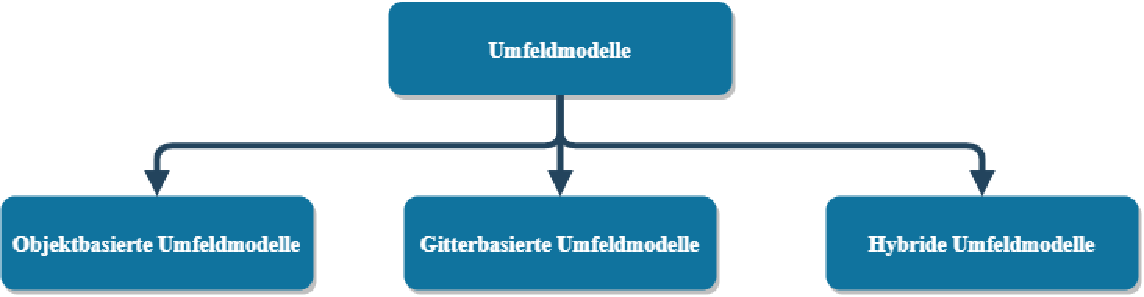
\includegraphics[width=1.0\textwidth]{pics/Umfeldmodelle_Klassen.pdf}
	\caption{M�gliche Umfeldmodelle f�r autonome Fahrzeuge}
	\label{fig:Umfeldmodelle_Klassen}
\end{figure}
Wie in Abbildung~\ref{fig:Umfeldmodelle_Klassen} dargestellt, stehen aktuell drei Hauptumweltmodelle in der Forschungs- und Automobilindustrie zur Verf�gung~\citep{Hegerhorst.2018}. Sie sind objektbasierte Umfeldmodelle, gitterbasierte Umfeldmodelle und hybride Umfeldmodelle. In den folgenden Abschnitten werden sie vorgestellt.
\subsubsection{Objektbasierte Modelle}
Objektbasierte Modelle werden auch als merkmalsbasierte Umfeldmodelle (engl. landmark-based oder feature map) bezeichnet~\citep{Thrun.2005}. Hierbei werden die Merkmalen, die f�r Erfassung der Umgebung g�nstig sind, durch Modelle beschrieben werden~\citep{Wurm.2010}. Au�erdem sollten die Merkmalen zuverl�ssig beobachtet und gemessen werden~\citep{Buschka.2005}. Die Modelle werden im Praxis als bestimmte Objektklasse beschrieben. Jede Klasse wird mit hervorragenden und ma�geblichen Eingenschaften versehen, die deutlich mittels zutreffenden Sensoren beobachtbar sind~\citep{Winner.2015}. F�r die Klassen lassen sich dar�ber hinaus die zu Objekt passende Geometrieformen bestimmen~\citep{Pieringer.2013}. Daher ist die Performance des Modells abh�ngig davon, ob die zu modellierten Objekte ausreichend pr�zis und einfach beschrieben werden k�nnen. Hierbei sind die Genauigkeit gegen der Zeit- und Speicheraufwand abzuw�gen. Ein Beispiel ist das in Abblidung~\ref{fig:FeatureMap} gezeigte Umfeldmodell. Auf der linken Seite sind Merkmale dargestellt und das Bild rechts zeigt das generierte Umfeldmodell.
\begin{figure}[htbp]
	\centering
	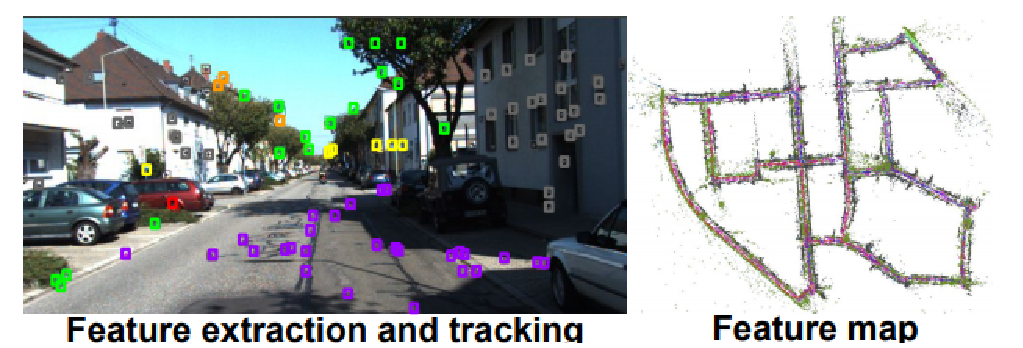
\includegraphics[width=1.0\textwidth]{pics/FeatureMap.pdf}
	\caption{Ein objektbasiertes Umfeldmodell~\citep{FawadAhmad.2020}}
	\label{fig:FeatureMap}
\end{figure}
\\Objektbasierte Umfeldmodelle sind vor allem geeignet f�r Szenen, wo die Objekte entweder im gro�en offenen Raum mit vordefinierten Merkmalen (z.B. Autobahn) oder dynamisch und einfach modelliert (z.B. Fu�g�nger oder Fahrzeuge) sind~\citep{Hegerhorst.2018}~\citep{Wurm.2010}. Da es im Rahmen dieser Arbeit ein statisches Umfeld im urbanen Raum angeht, ist dieses Modell unangemessen und sollte daher verzichtet werden.  
\subsubsection{Gitterbasierte Modelle}
\label{Abschnitt:Gitterbasierte Modelle}
In gitterbasierten Modellen wird die zentrale Idee der probabilistischen Robotik eingef�hrt, um die Wahrscheinlichkeitsverteilung unbeobachteter Zust�nde eines Systems mit gegebenen Beobachtungen und Messungen zu absch�tzen. Zur Modellierung des Umfelds ist der zentrale und entscheidende Zustand der sogenannte Belegungszustand. Der Belegungszustand erweist sich, ob eine Gitterzelle belegt ist. Daraus ergibt sich eine Zufallsvariable X, den Belegungszustand repr�sentiert. Die Variable X kann zwei Werte annehmen, welche 0 und 1 sind. Die entsprechen dabei, dass die Gitterzelle frei und belegt ist.
\\Das Modell, welches auf der obenerw�hnten Idee aufbaut, wird als Occupancy Grid beschrieben. Das Occupancy Grid ist ein mehrdimensionales Zufallsfeld, das zum Speichern einer stochastischen Sch�tzung des Belegungszustands jeder Zelle im r�umlichen Gitter verwendet wird~\citep{Elfes.1989}. Wie in Abbildung~\ref{fig:EbeneVonOccupancyGrid} gezeigt, l�sst sich Occupancy Grid in zwei Ebenen zerlegen.
\begin{figure}[htbp]
	\centering
	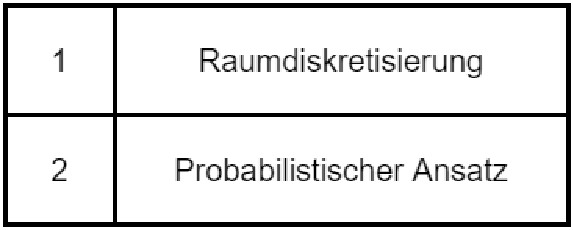
\includegraphics[width=0.5\textwidth]{pics/Ebene von Occupancy Grid.pdf}
	\caption{Zwei Ebenen von Occupancy Grid}
	\label{fig:EbeneVonOccupancyGrid}
\end{figure}
\\Auf der ersten Ebene wird die Raumdiskretisierung ausgef�hrt. Im Rahmen dieser Arbeit wird das Umfeld als zweidimensionaler Raum dargestellt. Die Diskretisierung des Raums bedeutet hierbei, dass die Fahrzeugumgebung durch ein Raster diskreter und fester Gr��e dargestellt wird~\citep{Hegerhorst.2018}. Die grafische Darstellung ist in Abbildung~\ref{fig:Raumdiskretisierung} gezeigt. Zu jeder Zelle wird au�erdem zus�tzliche Informationen hinzugef�gt. In Hinsicht auf Umfeldmodellierung ist die entscheidende Information der Belegungszustand der Zelle. Zur Vereinfachung der Modellierung, wird eine Annahme auf dieser Ebene zugleich getroffen, dass der Belegungszustand einer Gitterzelle ist unabh�ngig von diejenige der Nachbarzellen. Obwohl diese Annahme mit der Realit�t unvereinbar zu sein scheint, ist es erwiesen, dass Occupancy Grid Modell in der Praxis unter dieser Annahme robust ist und zudem die Rechenkomplexit�t reduzieren kann~\citep{Thrun.2005}.
\begin{figure}[htbp]
	\centering
	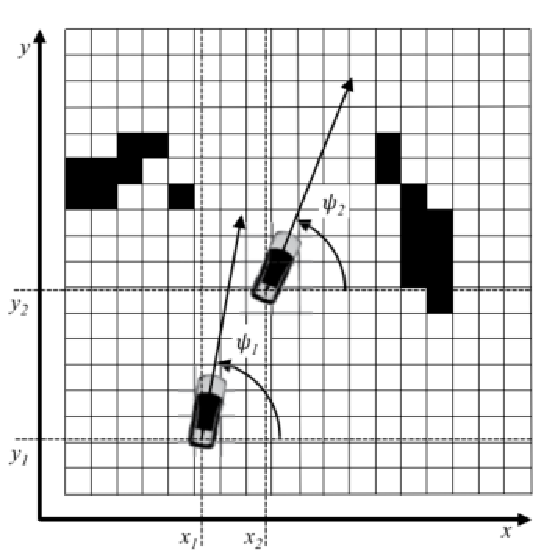
\includegraphics[width=0.5\textwidth]{pics/Raumdiskretisierung.pdf}
	\caption{Raumdiskretisierung der Umgebung um Fahrzeug \citep{Winner.2015}}
	\label{fig:Raumdiskretisierung}
\end{figure}
\\Auf der zweiten Ebene ist der probabilistische Ansatz eingef�hrt, welcher aus dem Themengebiet von Robotik stammt~\citep{Pieringer.2013}. Der Ansatz beruht auf Raumdiskretisierung und wird in der Praxis f�r jede einzelne Zelle eingesetzt. Der Ansatz l�sst sich, wie in Abbildung~\ref{fig:OccupancyGrid} gezeigt, in viele Komponenten unterteilen. Im Zentrum des Modells steht ein Algorithmus-Framework, das als bin�rer Bayes-Filter oder der bin�re Bayessche Filter (engl. Binary Bayes Filter) bekanntlich ist. Die Eingaben des Frameworks umfassen Messungswerte, inverses Sensormodell und Anfangsbedienungen. Die Ausgabe ist A-posteriori-Wahrscheinlichkeit von dem Zufallsereignis, die M�glichkeit repr�sentiert, dass eine Zelle als besetzt betrachtet wird. Um die Konzept von Occupancy Grid zu verdeutlichen, wird im Folgenden auf jede Komponente vertieft eingegangen.
\begin{figure}[htbp]
	\centering
	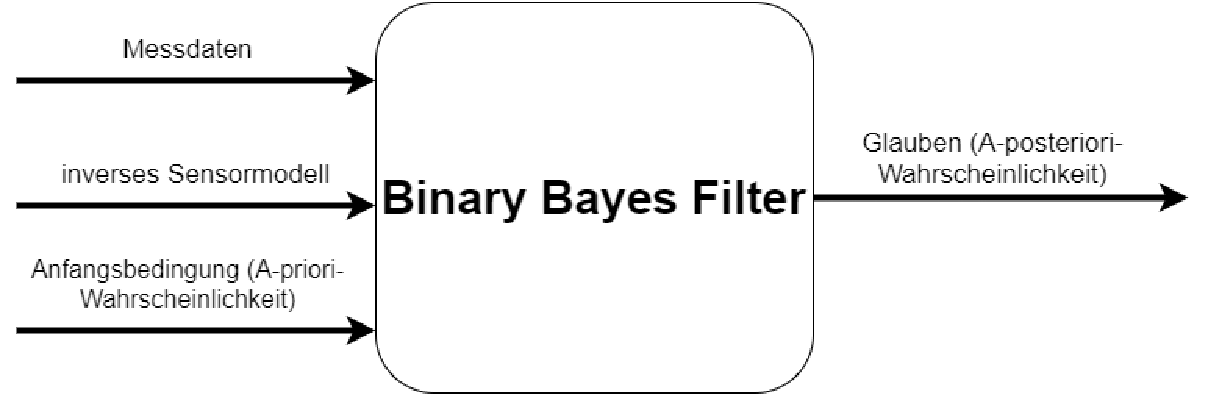
\includegraphics[width=1.0\textwidth]{pics/OccupancyGrid.pdf}
	\caption{Bestandteile des Modells Ocuupancy Grid}
	\label{fig:OccupancyGrid}
\end{figure}
\\Der Bayessche Filter ist zuerst zu beleuchten, mit dem die Funktionen und Bedeutungen der anderen Bestandteilen des Modells eng verbunden sind. Der Bayes-Filter ist eine rekursive Berechnungsvorschrift zur Sch�tzung von Wahrscheinlichkeitsverteilungen unbeobachteter Zust�nde eines Systems mit gegebenen Beobachtungen und Messungen~\citep{Thrun.2005}. Die Zustandssch�tzung befasst sich mit dem Problem der Sch�tzung von Gr��en, die nicht direkt beobachtbar sind, sondern abgeleitet aus den Sensordaten werden k�nnen. Das Ziel ist den Zustand $x$ eines Systems zu sch�tzen\footnote{Pr�zis sollte die Formel $X=x$ verwendet, um den Zustand zu beschreiben, wobei X eine Zufallsvariable ist und x ist der spezifische Wert, den X in Echtzeit annimmt. Zur Vereinfachung der Notation wird die Formel $X=x$ im Rahmen dieser Arbeit sowie in vielen Literaturen als $x$ bezeichnet.}, wenn Beobachtung $z$ und Kontrolle u angegeben sind. Das hei�t, die in Gleichung~\ref{Gleichung:Zustandschaetzung} gezeigte mathematische Formel sollte bestimmt werden. Hierbei entspricht $x_t$ dem Zustand zum Zeitpunkt t. $z_{1:t}$ bezeichnet die Beobachtungen bzw. die Messgr��en von den Zust�nden, die sich von Zeitstempel 1 bis t erstrecken. Zudem gibt $u_{1:t}$ die Kontrollen an, die sich von Zeitstempel 1 bis t erstrecken. Die linke Seite der Gleichung $bel_(x_t)$ verk�rpert den Glauben (engl. belief) der Wahrheit, dass der Zustand $x_t$ ist~\citep{Thrun.2005}.
\begin{equation}\label{Gleichung:Zustandschaetzung}
	bel(x_t)=p(x_{t}|z_{1:t},u_{1:t})
\end{equation}
Um die Wahrscheinlichkeitsverteilung einzugehen und eine rekursive Form zu entdecken, wird der stochastische Prozess von Zustands�nderung als Hidden Markov Model (HMM) betrachtet, das auch als dynamic Bayes network (DBN) bezeichnet wird. Unter Anwendung dieser Annahme gilt: Die Wahrscheinlichkeit eines Zustands bei dem Zeitstempel $t$ ist einschlie�lich abh�ngig von Zustand bei dem Zeitstempel $t-1$ und nicht von Zust�nden bei den Zeitstempeln, die fr�her als $t-1$ sind. Mathematisch wird HMM als eine Gleichung in~\ref{Gleichung:HMM} beschrieben.
\begin{equation}\label{Gleichung:HMM}
 	p(x_{t}|x_{1:t})=p(x_t|x_{t-1}) 
\end{equation}
Au�erdem beschreibt Hidden Markov Model, wie in Abbildung~\ref{fig:HiddeMarkovModel} dargestellt, die vereinfachte Zusammenhang zwischen dem Zustand $x$, der Messgr��e $z$ und der Kontrolle $u$. Der Zustand zum Zeitpunkt $t$ ist abh�ngig von dem Zustand zum Zeitpunkt $t-1$ und der Kontrolle $u_t$. Die Messgr��e $z_t$ h�ngt stochastisch vom Zustand zum Zeitpunkt $t$ ab.
\begin{figure}[htbp]
	\centering
	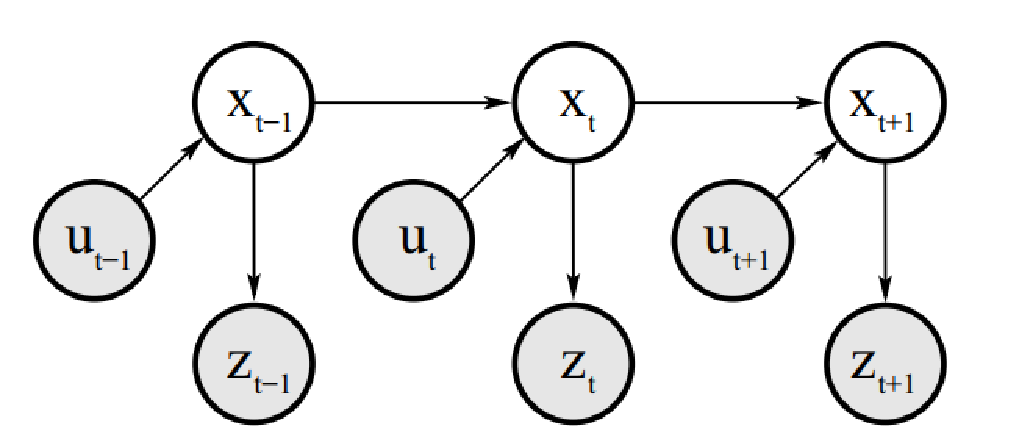
\includegraphics[width=0.5\textwidth]{pics/HMM.pdf}
	\caption{Hidden Markov Model (HMM) \citep{Thrun.2005}}
	\label{fig:HiddeMarkovModel}
\end{figure}
Zus�tzlich wird unter Anwendung des Satzes von Bayes und des Gesetzes der totalen Wahrscheinlichkeit wird die Formel~\ref{Gleichung:Zustandschaetzung} in einen rekursiven Ausdruck abgeleitet, was als Bayes-Filter bekanntlich ist. Die Ableitung findet sich in~\citep{Thrun.2005} und wird hier weggelassen. Der daraus resultierte Algorithmus befinden sich in Tabelle~\ref{tab:AlgorithmBF}.
\begin{table}[ht]
	\caption{Der Algorithmus des Bayes-Filters~\cite{Thrun.2005}}
	\small
	\centering
	\label{tab:AlgorithmBF}
	\begin{tabular}{ll}
		\toprule
		\textbf{Algorithm Bayes Filter($bel(x_{t-1}),u_t,z_t$):}\\
		for all $x_t$ do\\
		~~~~$\overline{bel}(x_t)=\int{p(x_t|u_t,x_{t-1})bel(x_{t-1})dx_{t-1}}$\\ 	
		~~~~$bel(x_t)=\eta p(z_t|x_t)\overline{bel(x_t)}$\\	
		endfor\\
		return $bel(x_t)$\\		
		\toprule
	\end{tabular}
\end{table}
Der Algorithmus besteht aus 2 Schritten, die als Pr�diktion (engl. prediction) und Korrektur (engl. Correction oder update) bekanntlich sind. Der erste Schritt wird dadurch ausf�hrt, dass der Glauben bzw. die Wahrscheinlichkeitsverteilung �ber den Zustand $x_t$ - basierend auf dem vorherigen Glauben �ber den Zustand $x_{t-1}$ und Kontrolle $u_t$ - berechnet werden sollte. Der zweite Schritt ist eine Korrektur bzw. ein Update des prognostizierte Glaubens, indem die beobachte Informationen des Zustands bzw. die Messgr��en der Sensoren fusioniert und ber�chtigt werden. Der Wert $bel(x_t)$ wird als A-posteriori-Verteilung bezeichnet. Im Gegensatz zu A-priori-Verteilung verk�rpert A-posteriori-Verteilung den theoretisch pr�ziseren Glauben, nachdem die Messgr��en von Sensoren durch ein Sensormodell zur Genauigkeit des Glaubens beitragen. Dieser Algorithmus bildet eine Grundlage, auf der viele weitere Algorithmen f�r bestimmte Szenarien entwickelt werden. Dazu geh�ren bekannte Gau�-Filter mit ihren Varianten, Particle-Filter und der diskrete Bayes-Filter. Der bin�re Bayes-Filter, der in dieser Arbeit eine gro�e Rolle spielt, ist ein spezieller Fall des Bayes-Filters bzw. des diskreten Bayes-Filter.
\\Der bin�re Bayes-Filter, der durch den grundlegenden Bayes-Filter eingef�hrt wird, erfordert eine Annahme. Es wird angenommen, dass der Zustand einschlie�lich zwei M�glichkeiten besitzen. Das hei�t, die Zufallsvariable, die den Zustand repr�sentiert, kann nur zwei Werte annehmen. Bei Occupancy Grid kann der wichtigste und auch einzige Zustand der Belegungszustand sein, der lediglich zwei F�lle - belegt oder frei - hat. Aus diesem Grund ist der bin�re Bayes-Filter daf�r zutreffend. Dar�ber hinaus wird eine weitere Annahme getroffen, dass der Belegungszustand bei Occupancy Grid statisch ist. Dies bedeutet, dass sich der Belegungszustand im Laufe der Zeit nicht �ndert und die Kontrolle $u$ hat keine Auswirkung auf den Belegungszustand. Somit wird das Schema des stochastischen Prozesses der Zustandsver�nderung von Abbildung~\ref{fig:HiddeMarkovModel} nach Abbildung~\ref{fig:reducedHMM} vereinfacht, indem die Kontrollen ausgeklammert werden. Nach diesen beiden Annahmen ist klar, dass der Algorithmus des Bayes-Filters in Occupancy Grid den Schritt Pr�diktion nicht mehr enth�lt. Die A-posteriori-Verteilung der Zustand $bel(x_t)$ ist einschlie�lich berechnet mit Informationen von Messdaten und dem vorherigen Zustand $bel(x_{t-1})$.
\begin{figure}[htbp]
	\centering
	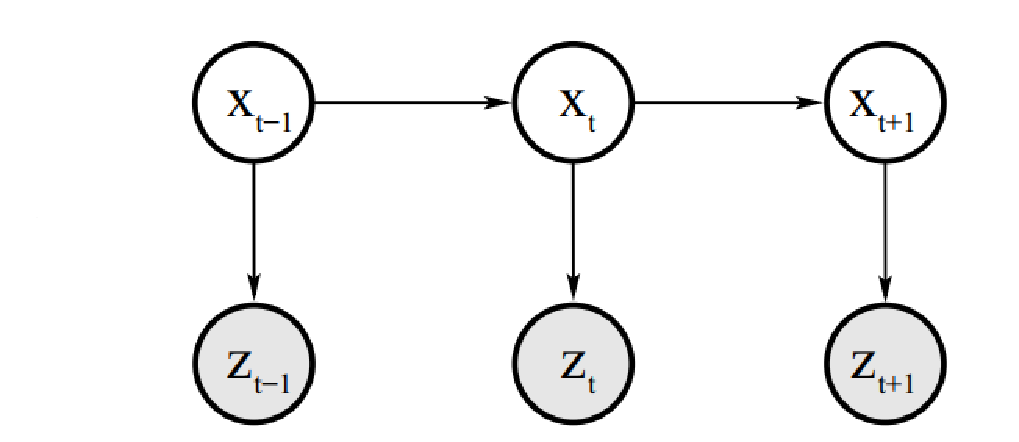
\includegraphics[width=0.5\textwidth]{pics/reducedHMM.pdf}
	\caption{Das reduzierte HMM \citep{Thrun.2005}}
	\label{fig:reducedHMM}
\end{figure}
\\Anhand der Vereinfachung des Modells sollte der grundlegende Bayes-Filter entsprechend vereinfacht werden. Au�erdem sollte der vereinfachte Algorithmus ein inverses Sensormodell verwenden. Das inverse Sensormodell gibt anstatt $p(z_t|x)$ eine Verteilung �ber die bin�re Zustandsvariable als Funktion der Messung $p(x|z_t)$ an \citep{Thrun.2005}. Ein Grund f�r die Verwendung des inversen Sensormodells ist die Leichtigkeit, eine Funktion zu entwickeln, die die Wahrscheinlichkeitsverteilung von Sensordaten berechnet. Es ist zum Beispiel relativ simpel ein Modell zu entwerfen, womit die Wahrscheinlichkeit des Belegungszustands einer Zelle oder mehrerer Zellen anhand der Sensordaten bestimmt werden kann. Ein Vorw�rtssensormodell ist dagegen in diesem Fall erstaunlich schwierig. Mit dem Ziel, einen vereinfachten Algorithmus zu finden, der unter Verwendung eines inversen Sensormodells das Glauben $bel(x_t)$ berechnen kann, sollte die mathematische Ableitung nach ~\citep{Thrun.2005}~\cite{Weiss.1306200715062007}~\citep{Hegerhorst.2018} folgend vorgestellt.
\\Da der Belegungszustand statisch ist und die Kontrolle $u$ somit ignoriert wird, kann die Gleichung~\ref{Gleichung:Zustandschaetzung} in eine vereinfachte Gleichung~\ref{Gleichung:Glauben} umgewandelt werden.
\begin{equation}
	\label{Gleichung:Glauben}
	bel(x_t)=p(x_t|z_{1:t},u_{1:t})=p(x_t|z_{1:t})
\end{equation}
Bei Occuancy Grid ist der interessierende Zustand der Belegungszustand. Zur Vereinfachung der Notation wird das Glauben, dass die Zelle i des Gitters zum Zeitpunkt t belegt ist, als Gleichung~\ref{Gleichung:Glauben_belegt} bezeichnet.
\begin{equation}
	\label{Gleichung:Glauben_belegt}
	bel_t(m_i)=p(m_i|z_{1:t})
\end{equation}
Analog daf�r ergibt sich das Glauben, dass die Zelle i des Gitters zum Zeitpunkt t frei ist, aus Gleichung ~\ref{Gleichung:Glauben_frei}.
\begin{equation}
	\label{Gleichung:Glauben_frei}
	bel_t(\overline{m_i})=p(\overline{m_i}|z_{1:t})
\end{equation}
Mit Hilfe des bedingten Satzes der Bayes ergibt sich die Gleichung~\ref{Gleichung:Glauben_belegt} zu
\begin{equation}
	\label{Gleichung:Ableitung_01}
	bel_t(m_i)=p(m_i|z_{1:t})=\frac{p(z_t|m_i,z_{1:t-1})p(m_i|z_{1:t-1})}{p(z_t|z_{1:t-1})}
\end{equation}
Unter Annahme eines Hidden-Markov-Modells wird die Gleichung~\ref{Gleichung:Ableitung_01} zu
\begin{equation}
	\label{Gleichung:Ableitung_02}
	bel_t(m_i)=\frac{p(z_t|m_i,z_{1:t-1})p(m_i|z_{1:t-1})}{p(z_t|z_{1:t-1})}=\frac{p(z_t|m_i)p(m_i|z_{1:t-1})}{p(z_t|z_{1:t-1})}
\end{equation}
Zur Wahrscheinlichkeit $p(z_t|m_i)$ wird der Satz des Bayes wiederum eingesetzt, womit die Gleichung~\ref{Gleichung:Ableitung_02} wird zu
\begin{equation}
	\label{Gleichung:Ableitung_03}
	bel_t(m_i)=\frac{p(z_t|m_i)p(m_i|z_{1:t-1})}{p(z_t|z_{1:t-1})}=\frac{p(m_i|z_t)p(z_t)p(m_i|z_{1:t-1})}{p(m_i)p(z_t|z_{1:t-1})}
\end{equation}
Analog dazu hat der gegenteilige Zustand den Glauben
\begin{equation}
	\label{Gleichung:Ableitung_04}
	bel_t(\overline{m_i})=1-bel_t(m_i)=\frac{p(z_t|\overline{m_i})p(\overline{m_i}|z_{1:t-1})}{p(z_t|z_{1:t-1})}=\frac{p(\overline{m_i}|z_t)p(z_t)p(\overline{m_i}|z_{1:t-1})}{p(\overline{m_i})p(z_t|z_{1:t-1})}
\end{equation}
Dividiert Gleichung~\ref{Gleichung:Ableitung_03} durch der Gleichung~\ref{Gleichung:Ableitung_04}, so ergibt sich
\begin{equation}
	\label{Gleichung:Ableitung_05}
	\frac{bel_t(m_i)}{1-bel_t(m_i)}=\frac{p(m_i|z_t)}{1-p(m_i|z_t)}\frac{p(m_i|z_{1:t-1})}{1-p(m_i|z_{1:t-1})}\frac{1-p(m_i)}{p(m_i)}
\end{equation}
Die Gleichung~\ref{Gleichung:Ableitung_05} bietet eine perfekte mathematische Darstellung bzw. Erkl�rung an, was die Angaben und die Ausgabe des bin�ren Bayes-Filters sind. Die Ausgabe ist das Glauben bzw. die A-posteriori-Wahrscheinlichkeit des Ereignisses, dass die Zelle $m_i$ belegt ist, welches den Term $bel_t(m_i)$ in Gleichung~\ref{Gleichung:Ableitung_05} entspricht. Der Term ${p(m_i|z_t)}$ ist, wie oben erz�hlt, das inverse Sensormodell. Es ist ersichtlich, dass eine bedeutende Beziehung zwischen dem Sensormodell bzw. der Beschreibung des Sensormodells und dem Sensortyp. Darauf wird in Abschnitt~\ref{Abschnitt:Sensor} mit der Erfassung der Umgebung vertieft eingegangen. Der Term $p(m_i|z_{1:t-1})$ beweist dabei das wichtige Merkmal des bin�ren Bayes-Filters, dass das Verfahren der Sch�tzung auf Rekursion beruht. Die Anfangsbedingung bzw. die A-priori-Wahrscheinlichkeit wird als Term $p(m_i)$ in Gleichung~\ref{Gleichung:Ableitung_05} bezeichnet. Die A-priori-Wahrscheinlichkeit gibt den Glauben an, vordem alle Messdaten von Sensorik ber�cksichtigt werden. Typischerweise wird bei Occupancy Grid anf�nglich $p_(m_i)$ ein Wert von 0,5 angegeben, weil es zu Beginn keine Information �ber den Belegungszustand gibt. Die Wahrscheinlichkeit, dass eine Gitterzelle belegt ist, ist die gleiche wie die Wahrscheinlichkeit, dass sie nicht belegt ist. Daher wird die Gleichung~\ref{Gleichung:Ableitung_05} zu
\begin{equation}
	\label{Gleichung:Ableitung_06}
	bel_t(m_i)=\frac{Y}{Y+1}
\end{equation}
mit
\begin{equation*}
	\label{Gleichung:Ableitung_07}
	Y=\frac{p(m_i|z_t)}{1-p(m_i|z_t)}\frac{p(m_i|z_{1:t-1})}{1-p(m_i|z_{1:t-1})}
\end{equation*}
Zusammenfassend ist das gitterbasierte Modell eignet f�r eine statische Umgebung im urbanen Raum. Au�erdem bietet das Modell einen Vorteil, einen Freiraum neben belegten Objekten zu modellieren, was eine Grundlage der darauffolgenden Navigation schaffen.
\subsubsection{Hybride Umfeldmodelle}
Um ein Umfeld zu modellieren, welches komplizierte Szenarien repr�sentieren kann, werden selbstverst�ndlich Hybride Umfeldmodelle aufgefordert. Dadurch werden die Einschr�nkungen der beiden vorherigen Basismodelle eliminiert und ihre Vorteilen ausgenutzt. Es gibt unterschiedliche Kriterien und Methoden zum Erstellen eines hybriden Umfeldmodells. Das~\cite{.0612201908122019} betreffende Modell, ist ein beliebtes Beispiel von hybriden Umfeldmodellen. Im Prinzip ist das Modell eine Kombination von einem objektbasierten Umfeldmodell und einem gitterbasierten Umfeldmodell. Hierbei beschreibt das objektbasierte Umfeldmodell dynamische Objekte, wohingegen das gitterbasierten Umfeldmodell bzw. Occupancy Grid den statischen Raum darstellen. Auf diese Weise ist das fusionierte Modell generell in der Lage eine Umgebung, wo sich dynamische und statischen Objekte befinden, vollst�ndig und zutreffend zu beschreiben. Dar�ber hinaus kann die objektbasierte Umfeldmodellierung mit aktueller Technik z.B. Deep-Learning pr�ziser und effizienter durchgef�hrt werden, w�hrend die semantische Navigation weiterhin direkt im gitterbasierten Umfeldmodell verlaufen kann\cite{.0612201908122019}. Da das Umfeld im Rahmen dieser Arbeit als statische Umgebung betrachtet wird, wird ein Hybrides Umfeldmodell aufgrund seiner Komplexit�t und Redundanz nicht verwendet.
\subsection{Sensorik und ihr inverses Sensormodell}
\label{Abschnitt:Sensor}
Zweifellos dient Wahrnehmung bzw. Erfassung als eine wichtige Voraussetzung f�r Umfeldmodelleirung, weil sie die Informationsquelle bietet. Die Wahrnehmung eines Fahrzeugs umfasst im Wesentlichen die Bestimmung der eigenen Position samt Orientierung und die Abtastung der Umgebung um das Fahrzeug. Die Eingenlokalisierung ist im Rahmen dieser Arbeit nebens�chlich und durch die vorgegebene GPS-Information bestimmt. Darauf soll in dieser Arbeit nicht n�her eingegangen werden. In diesem Abschnitt liegt der Schwerpunkt auf den Sensoren, mit denen die Umgebung modelliert wird. Dar�ber hinaus werden die von IfF-Versuchsfahrzeug verwendeten Laserscanner und das in Abschnitt~\ref{Abschnitt:Gitterbasierte Modelle} erw�hnte inverse Sensormodell erl�utert.
\subsubsection{�berblick �ber die verschiedenen Sensoren zur Umfeldmodellierung}
Um ein zuverl�ssiges Umfeldmodell zu entwickeln und das Modell danach in der Praxis effektiv umzusetzen, spielt die Auswahl der erfassenden Sensoren entweder in der Akademie oder in der Industrie eine gro�e Rolle. Die wichtigsten und am weitesten verbreiteten Fahrzeugsensoren zur Wahrnehmung der Umgebung sind Kameras, fernes Infrarot- (engl.Far-infrared, als FIR abgek�rzt) Radar-, LiDAR (Light Detection and Ranging)- und Ultraschallsensoren. Nach~\citep{Mohammed.2020} sind die Vorteilen neben der Nachteilen in Tabelle~\ref{tab:Vergleich der Sensoren} aufgelistet.
\\Es ist erw�hnenswert, dass Kameras aufgrund ihrer niedrigen Preise akademisch und industriell beliebt sind. Es wird h�ufig verwendet, um objektbasierte Umfeldmodelle mithilfe von Computer Vision zu erstellen. Immer mehr Algorithmen werden entwickelt, um die Tiefeninformation von Bildern zu berechnen. Obwohl die Erkennungsqualit�t begrenzt ist, wurde aus historischen Gr�nden eine gro�e Anzahl von Radarger�ten an Testfahrzeugen angebracht, sodass die Radar-basierte Forschung und Entwicklung noch nicht abgeschlossen ist. Der Preis von LiDAR-Senor ist relativ hoch, aber sein absoluter Vorteil liegt in der Genauigkeit und Aufl�sung von Tiefeninformationen und Positionsinformationen, und es eignet sich f�r die Erstellung von Occupancy Grid.
\\Im Rahmen dieser Arbeit ist die am IfF bereits bestehende Fahrzeugarchitektur mit Ibeo-LUX-Laserscanner versehen. Daher werden folgend in Abschnitt~\ref{Abschnitt:Laserscanner} der Mechanismus des Laserscanners und das daraus resultierende Sensormodell erl�utert. Au�erdem werden die technische Details bei Einf�hrung der inversen Sensormodellierung vorgestellt, weil die realen technischen Gr��en dabei ein wichtiger Faktor sind.
\begin{longtable}[htbp]{|m{0.15\textwidth}<{\centering}|m{0.4\textwidth}<{\centering}|m{0.4\textwidth}<{\centering}|}
	\caption{Vorteile und Nachteile von Kamera, fernes Infrarotsensor,  Radar-, Ultraschall- und Lidarsensor~\citep{Mohammed.2020}}
	\centering
	\label{tab:Vergleich der Sensoren}
	\endfirsthead
	\endhead
	\hline	
	\textbf{Sensor} & \textbf{Vorteile} & \textbf{Nachteile}\\ \hline
	Kamera& 
	\begin{itemize}  
		\setlength\itemsep{0em} 
		\item eine hohe Aufl�sung und Farbskalen �ber das gesamte Sichtfeld haben 
		\item eine farbenfrohe Perspektive der Umgebung bieten 
		\item eine 3D-Geometrie von Objekten bei Stereokameras bereitstellen
		\item kosteng�nstig Im Vergleich zu Lidar sind
	\end{itemize}&
	\begin{itemize}  
		\setlength\itemsep{0em} 
		\item ein leistungsf�higes Berechnungssystem ben�tigen, um n�tzliche Daten zu extrahieren 
		\item empfindlich auf starken Regen, Nebel und Schneefall reagieren 
		\item eine 3D-Geometrie von Objekten bei Stereokameras bereitstellen
		\item begrenzte Reichweite besitzen
	\end{itemize} 
	\\ \hline
	
	FIR-Sensor& 
	\begin{itemize}  
		\setlength\itemsep{0em} 
		\item nicht von der Lichtbedingungen und Objektoberfl�chenmerkmale beeinflusst werden k�nnen
		\item eine bessere Sicht durch Staub, Nebel und Schnee als Kameras  haben 
		\item eine horizontale Erfassungsreichweite bis zu 200m oder mehr abdecken 
		\item im Vergleich zu Lidar billiger und kleiner sind
	\end{itemize}&
	\begin{itemize}  
		\setlength\itemsep{0em} 
		\item anspruchsvolle Rechenquellen und robuste Algorithmen erfordern
		\item schwierig Ziele in Szenarien mit kaltem Klima zu unterscheiden  
		\item niedrigere Aufl�sung im Vergleich zur sichtbaren Kamera haben
		\item keine Information �ber Entfernung bieten
	\end{itemize} 
	\\ \hline
	
	Radarsensor& 
	\begin{itemize}  
		\setlength\itemsep{0em} 
		\item lange Strecken bei schlechten Sichtverh�ltnissen vor dem Auto sehen 
		\item klein, leicht und erschwinglich sind 
		\item weniger Strom als ein Lidar-Sensor ben�tigen
		\item im Vergleich zu Lidar robuster gegen Ausf�lle sind
	\end{itemize}&
	\begin{itemize}  
		\setlength\itemsep{0em} 
		\item eine geringe Genauigkeit und Aufl�sung bieten
		\item begrenzte Informationen  (z. B. weder genaue Form- noch Farbinformationen) bekommen
		\item das Problem wegen der gegenseitigen Beeinflussung von Radarsensoren haben
		\item schlechte Azimut- und H�henaufl�sung verf�gen
		\item ohne einer Erh�hung der Leistung Radard�mpfung zeigen
	\end{itemize} 
	\\ \hline
	
	Ultraschall-\newline sensor & 
	\begin{itemize}  
		\setlength\itemsep{0em} 
		\item lange Strecken bei schlechten Sichtverh�ltnissen vor dem Auto sehen 
		\item klein, leicht und erschwinglich sind 
		\item weniger Strom als ein Lidar-Sensor ben�tigen
		\item im Vergleich zu Lidar robuster gegen Ausf�lle sind
	\end{itemize}&
	\begin{itemize}  
		\setlength\itemsep{0em} 
		\item eine geringe Genauigkeit und Aufl�sung bieten
		\item begrenzte Informationen  (z. B. weder genaue Form- noch Farbinformationen) bekommen
		\item das Problem wegen der gegenseitigen Beeinflussung von Radarsensoren haben
		\item schlechte Azimut- und H�henaufl�sung verf�gen
		\item ohne einer Erh�hung der Leistung Radard�mpfung zeigen
	\end{itemize} 
	\\ \hline
	
	LiDAR-Sensor & 
	\begin{itemize}  
		\setlength\itemsep{0em} 
		\item gro�e Entfernungen vor dem Auto bei guten Sichtverh�ltnissen erfassen
		\item volle $360^\circ$- und 3D-Punktwolken bieten 
		\item eine gute Genauigkeit und Aufl�sung haben
		\item keine signifikanten Interferenzen bei mehreren Lidarsensoren haben
	\end{itemize}&
	\begin{itemize}  
		\setlength\itemsep{0em} 
		\item teurer als Radar und Kamera sind
		\item kleine Objekte (wie Dr�hte und Stangen) nicht entdecken k�nnen
		\item eine schlechte Kontrastunterscheidung bei der Erkennung nasser Oberfl�chen haben
		\item durch unterschiedliche klimatische Bedingungen beeinflusst werden
	\end{itemize} 
	\\ \hline
\end{longtable} 
\subsubsection{Funktionsweise des Lasersensors}
\label{Abschnitt:Laserscanner}
Ist ein angemessenes Sensormodell zu finden, ist es sinnvoll das Mechanismus, die Eingenschaften und die Gr�nde der Unsicherheit zu untersuchen. Die Angemessenheit hierbei bedeutet, dass eine Abw�gung bzw. ein Kompromiss immer nach verschiedenen Anwendungsszenarien gemacht werden muss. 
\\Laserscanner beruht auf dem Prinzip ToF (Time-of-flight). Nach diesem Prinzip wird die Entfernung zwischen dem zu erfassenden Ziel und Laserscanner dadurch berechnet, dass die Zeit gemessen wird, die ein Lichtimpuls ben�tigt, um von der Lichtquelle zum beobachteten Ziel und dann zum Detektor (normalerweise zusammen mit der Lichtquelle) zu gelangen~\citep{Siciliano.2008}. Im Prinzip ist Lasersensor �hnlich wie Radarsensor, wobei nur Infrarot-, Ultraviolett- oder Strahlen aus dem Bereich des sichtbaren Lichts anstelle von Mikrowellen eingesetzt werden~\citep{Winner.2015}. Die mathematische Beschreibung des Prinzips l�sst sich in Gleichung~\ref{Gleichung:Tof} darstellen. Dabei bezeichnet d den Abstand zwischen Lasersensor und dem zu erfassenden Objekt. Das Lichtgeschwindigkeit wird als c dargestellt. Bei einigen hochpr�zisen Lasersensoren wird Lichtausbreitungsmedium auch ber�cksichtigt und dazu wird c der Umgebung gem�� kompensiert. Zeit t ben�tigt das Licht um die Ausbreitungsstrecke zu decken, die doppelte Entfernung zwischen Laserscanner und Objekt ist. Die Zeit wird in der Tat gemessen und in Abstand d �bergef�hrt. Der Sensor sendet periodisch Lichtimpulse aus und berechnet die durchschnittliche Zielentfernung basierend auf der Zeit des R�ckimpulses~\citep{Siciliano.2008}.
\begin{equation}
	\label{Gleichung:Tof}
	d=\frac{c\cdot t}{2}
\end{equation}
Im Bereich des selbstfahrenden Fahren wird der Lichtpuls mit nicht nur eine Ausrichtung ausgestrahlt, weil ein relativ gro�er Beobachtungsbereich mehrere Lichtstrahlen erfordert, die in verschiedene Richtungen emittiert werden. Aktuell gibt es zwei verschiedene LiDAR-Systeme. Zum einen ist das feststehende Sensor, in dem mehrere Sende-/ Empfangseinheiten in unterschiedlichen Ausrichtungen angeordnet werden~\citep{Effertz.2009}. Zum anderen wird das rotierende LiDAR-System dadurch realisiert, dass der Lichtimpuls mittels einer drehbaren Spiegeleinheit abgelenkt wird~\citep{Effertz.2009}. Der in dieser Arbeit verwendete Laserscanner Ibeo-LUX geh�rt zu dem zweiten Sensorsystem.
\subsubsection{Theorie des inversen Sensormodells}
Die Aufgabe des inversen Sensormodells besteht darin, den in~\ref{Abschnitt:Gitterbasierte Modelle} erw�hnten mathematischen Ausdruck $p(m_i|z)$ zu finden, der die Wahrscheinlichkeitsverteilung des Belegungszustands der Zelle mit dem Index i beschreibt. Nach~\citep{Pieringer.2013} l�sst sich das inverse Sensormodell im Prinzip in drei Bestandteile zerlegen. Wie in Abbildung~\ref{fig:Bestandteile_Sensormodell} gezeigt, handelt es sich hierbei um Hinderniskartierung, Freiraummodellierung und Beschreibung unbekannter Gebiete.
\begin{figure}[htbp]
	\centering
	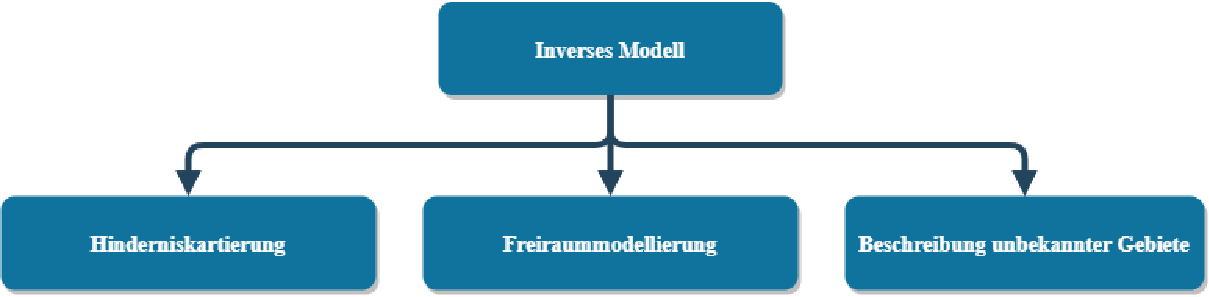
\includegraphics[width=1.0\textwidth]{pics/Bestandteile_Sensormodell.pdf}
	\caption{Bestandteile des Prinzips von Inverses Sensormodell }
	\label{fig:Bestandteile_Sensormodell}
\end{figure}
\\Unter Hinderniskartierung wird das Verfahren verstanden, dass die vom Sensor detektierten Objekte in das gitterbasierte Umfeldmodell bzw. das Occupancy Grid Map �bertragen werden~\citep{Pieringer.2013}. Zwei Probleme sind in diesem Bestandteil des inversen Sensormodells zu l�sen. Zum einen gewinnt es an Relevanz, welche Form f�r das detektierte Objekt bzw. das Hindernis angenommen wird~\citep{Pieringer.2013}. Die Form (z.B. Linie oder Ellipse), die das Hindernis repr�sentiert, ist theoretisch eng mit der Unsicherheitsquellen des Laserscanners verbunden. Jedoch wird die Form in der Praxis ausgew�hlt unter Ber�cksichtigung der Ausf�hrlichkeit bzw. Genauigkeit und Echtzeitanforderung. Zum anderen ist das Problem, mit welchem Zahlenwert die Wahrscheinlichkeit der kartierten Zelle erf�llt ist. Diese beiden Probleme werden nachstehend bei der tats�chlichen Sensormodellierung ausf�hrlicher er�rtert.
\\Freiraum ist bei dem Umfeldmodell der beobachtbare Bereich zwischen dem Sensor und dem erfassten Objekt. Analog zur Hinderniskartierung steht die Bestimmung der Form des Freiraums und der Wahrscheinlichkeit der betreffenden Zelle in Zentrum der Freiraummodellierung. Jedoch h�ngt die Form des Freiraums von der oben bestimmten Hindernisform. Beispielweise wird der Freiraum als Linie oder Dreiecke modelliert, wenn die Hindernisse punktf�rmig oder linief�rmig beschrieben werden. Bei Wahrscheinlichkeitsverteilung �ber den Freiraum spielt die Ursache der Unsicherheit eine gro�e Rolle. Mit zunehmender Entfernung wird beispielsweise die vom Laserscanner erkannte Entfernung zum Hindernis weniger zuverl�ssig. Aus diesem Grund ist dabei ein Modell zu entwickeln, die Unsicherheit in gewissem Grade widerspiegeln kann. In der Anwendung sind ebenso die Korrektheit und die Zeitaufwand zu gewichten.
\\Der Raum innerhalb der Reichweite des Laserscanners, der weder ein Hindernis noch ein freier Raum ist, ist ein unbekannter Bereich des Modells. Ein typisches Beispiel daf�r ist der Raum hinter hinter Hindernissen. Im Allgemeinen wird der Wahrscheinlichkeit einer unbekannten Zell als die A-priori-Wahrscheinlichkeit zugewiesen. Der Grund liegt darin, dass keine neuen Informationen �ber den Belegungszustand eingegeben werden. Typischerweise wird die A-priori-Wahrscheinlichkeit bzw. die Wahrscheinlichkeit einer unbekannten Zelle als $0,5$ zugewiesen.
\\Die obigen drei Teile werden nicht getrennt, sondern gleichzeitig in der tats�chlichen Implementierung ausgef�hrt. Das inverse Sensormodell ist einer der Schl�sselbestandteile von Occupancy Grid. Seine Genauigkeit und Einfachheit bestimmen die Qualit�t des Modells und den Zeitaufwand des Systems. In der Technik wird es h�ufig in Kombination mit tats�chlichen Anwendungsszenarien und Sensoreigenschaften erstellt.
\subsubsection{Technische Details von Ibeo-LUX}
In der am IfF bereits bestehenden Fahrzeugarchitektur werden Laserscanner Ibeo-LUX von Ibeo Automotive Systems GmbH f�r Erfassung der Umgebung um das selbstfahrende Fahrzeug verwendet. Das Golf 7 ist mit vier IBEO-LUX-4L ausgestattet. Neben 4 IBEO-LUX-4L Laserscannern sind auf der Vorder- und R�ckseite des Passat IBEO-LUX-8L-Laserscanner installiert. Um ein angemessenes Sensormodell f�r den Laserscanner zu entwickeln, ist es voraussetzt, dass die technische Details des Sensors zur Verf�gung stehen. Nach~\citep{IbeoAutomotiveSystemsGmbH.2017} sind die relevanten technischen Parameter in Tabelle~\ref{tab:technische Details von Ibeo LUX} aufgelistet.
\begin{table}[ht]
	\caption{Technische Details von Ibeo LUX}
	\label{tab:technische Details von Ibeo LUX}
	\centering
	\begin{tabular}{|c|c|}
		\hline
		\textbf{Technische Daten} & \textbf{Wert}\\
		\hline
		Reichweite & 50m mit $10\%$ Remission\\
		\hline
		Genauigkeit & 10cm\\
		\hline
		Entfernungsaufl�sung & 4cm\\
		\hline
		Horizontaler �ffnungswinkel & $110^\circ$ $(50^\circ$ bis $-60^\circ)$ \\
		\hline
		Vertikaler �ffnungswinkel & $6,4^\circ$ (LUX-8L) / $3,2^\circ$ (LUX-4L)\\
		\hline
		Horizontale Winkelaufl�sung & $0,25^\circ$\\
		\hline
		Vertikale Winkelaufl�sung & $0,8^\circ$\\
		\hline
		Bildrate & 25 Hz\\
		\hline
		Multi-Layer & 8 (LUX-8L) / 4 (LUX-4L)\\
		\hline
		Ausgabe & Punktwolke und Objektdaten\\
		\hline
		Abma�e (B$\times$T$\times$H) & 164,5$\times$93,2$\times$88mm\\
		\hline
		Gewicht & 998,7g\\
		\hline
	\end{tabular}
\end{table}
\subsubsection{Das zu verwendende Sensormodell}
Nach Einf�hrung der Theorie des inversen Sensormodells und der technischen Daten des verwendeten Ibeo-LUX-Laserscanners wird in diesem Abschnitt ein geeignetes Sensormodell entwickelt, um die Wirkung der Sensorinformation auf Glauben des Zellenbelegungszustands zu beschreiben. Hierbei wird ein Kompromiss zwischen Genauigkeit und Effizienz geschlossen. Aufgrund der Messunsicherheit und der in Tabelle~\ref{tab:technische Details von Ibeo LUX} aufgelisteten Laserscanner-Spezifikationen erfolgt die Sensormodellierung in zwei Schritten. Im ersten Schritt wird die Form des Hindernis mitsamt des entsprechenden Freiraums festgestellt. Darauffolgend wird es bestimmt, welcher Wahrscheinlichkeit in welchem Bereich zugewiesen wird~\citep{Pieringer.2013}.
\\Ein genaues Modell sollte die Wahrscheinlichkeit jeder Zelle in Abh�ngigkeit von der Position auf der Karte, der Strahlbreite und dem Abstand zum Zentrum des Strahls berechnen~\citep{Homm.2106201024062010}. Wenn die Positionsunsicherheit betr�chtlich ist, sollte eine kreis- oder ellipsenf�rmige Form f�r Hindernis unter Anwendung einer zweidimensionalen Gau�funktion angenommen werden~\citep{Pieringer.2013}. Steht eine niedrige Winkelaufl�sung eines Sensor zur Verf�gung, kann die Form zu einer Linie vereinfacht werden. Wenn der Sensor ausreichend genaue Tiefeninformationen hat, l�sst sich die Form weiter zu einem Punkt vereinfachen. 
\\Im Rahmen dieser Arbeit wird die Aufl�sung der Zelle als $0,1m$ zugewiesen. Au�erdem ist es sinnvoll, die maximale erfasste Entfernung $d_{max}$ des Laserscanners zu beschr�nken, obwohl laut Tabelle~\ref{tab:technische Details von Ibeo LUX} eine Reichweite 50m besteht.Dies kann die durch die gro�e Entfernung verursachte Unsicherheit verringern. Nach dem Test wird der Wert von $d_{max}$ als 10m bestimmt. Die horizontale Winkelaufl�sung $\Delta\theta$ betr�gt nach Tabelle~\ref{tab:technische Details von Ibeo LUX} $0,25^\circ$ oder 0,004363(rad). Durch Multiplizieren von $d_{max}$ und $\Delta\theta$ betr�gt der Wert des Kreisbogens $0,043$, der die wegen der Strahlbreite entstehende Divergenz beschreibt. Da $0,043<0,1$ gilt, l�sst sich der Einfluss von Strahlbreite vernachl�ssigen. Zudem wird angenommen, dass die Genauigkeit von $0,1m$ ausreichend genau ist. Damit ist es deutlich, dass Hindernisse im Rahmen dieser Arbeit aufgrund der Sensorspezifikation als Punkte beschrieben werden k�nnen. Daraus lassen sich herleiten, dass das entsprechende Freiraummodell als Linie dargestellt wird. Um ein Objekt zu detektieren, dessen Abmessung gr��er als Aufl�sung ist, ist der bekannte Begriff Raycasting zu einsetzen. Hierbei werden die einzelnen physikalischen Strahlen des Laserscanners zwischen dem Sensor und einem Objekt nachgebildet. Basierend darauf wird der n�chste Schritt der Modellierung eines Sensors simplifiziert und es wird nur erwartet, dass das inverse Sensormodell einziges Laserstrahls beschreiben kann. W�hrend der Implementierung werden alle Laserstrahlen mit demselben Sensormodell behandelt. Das inverse Modell eines einzelnen Strahls ist eindimensional und das von einem idealen Laserscanner verwendete Modell ist in Abbildung~\ref{fig:ideal_sensormodell} dargestellt. 
\begin{figure}[htbp]
	\centering
	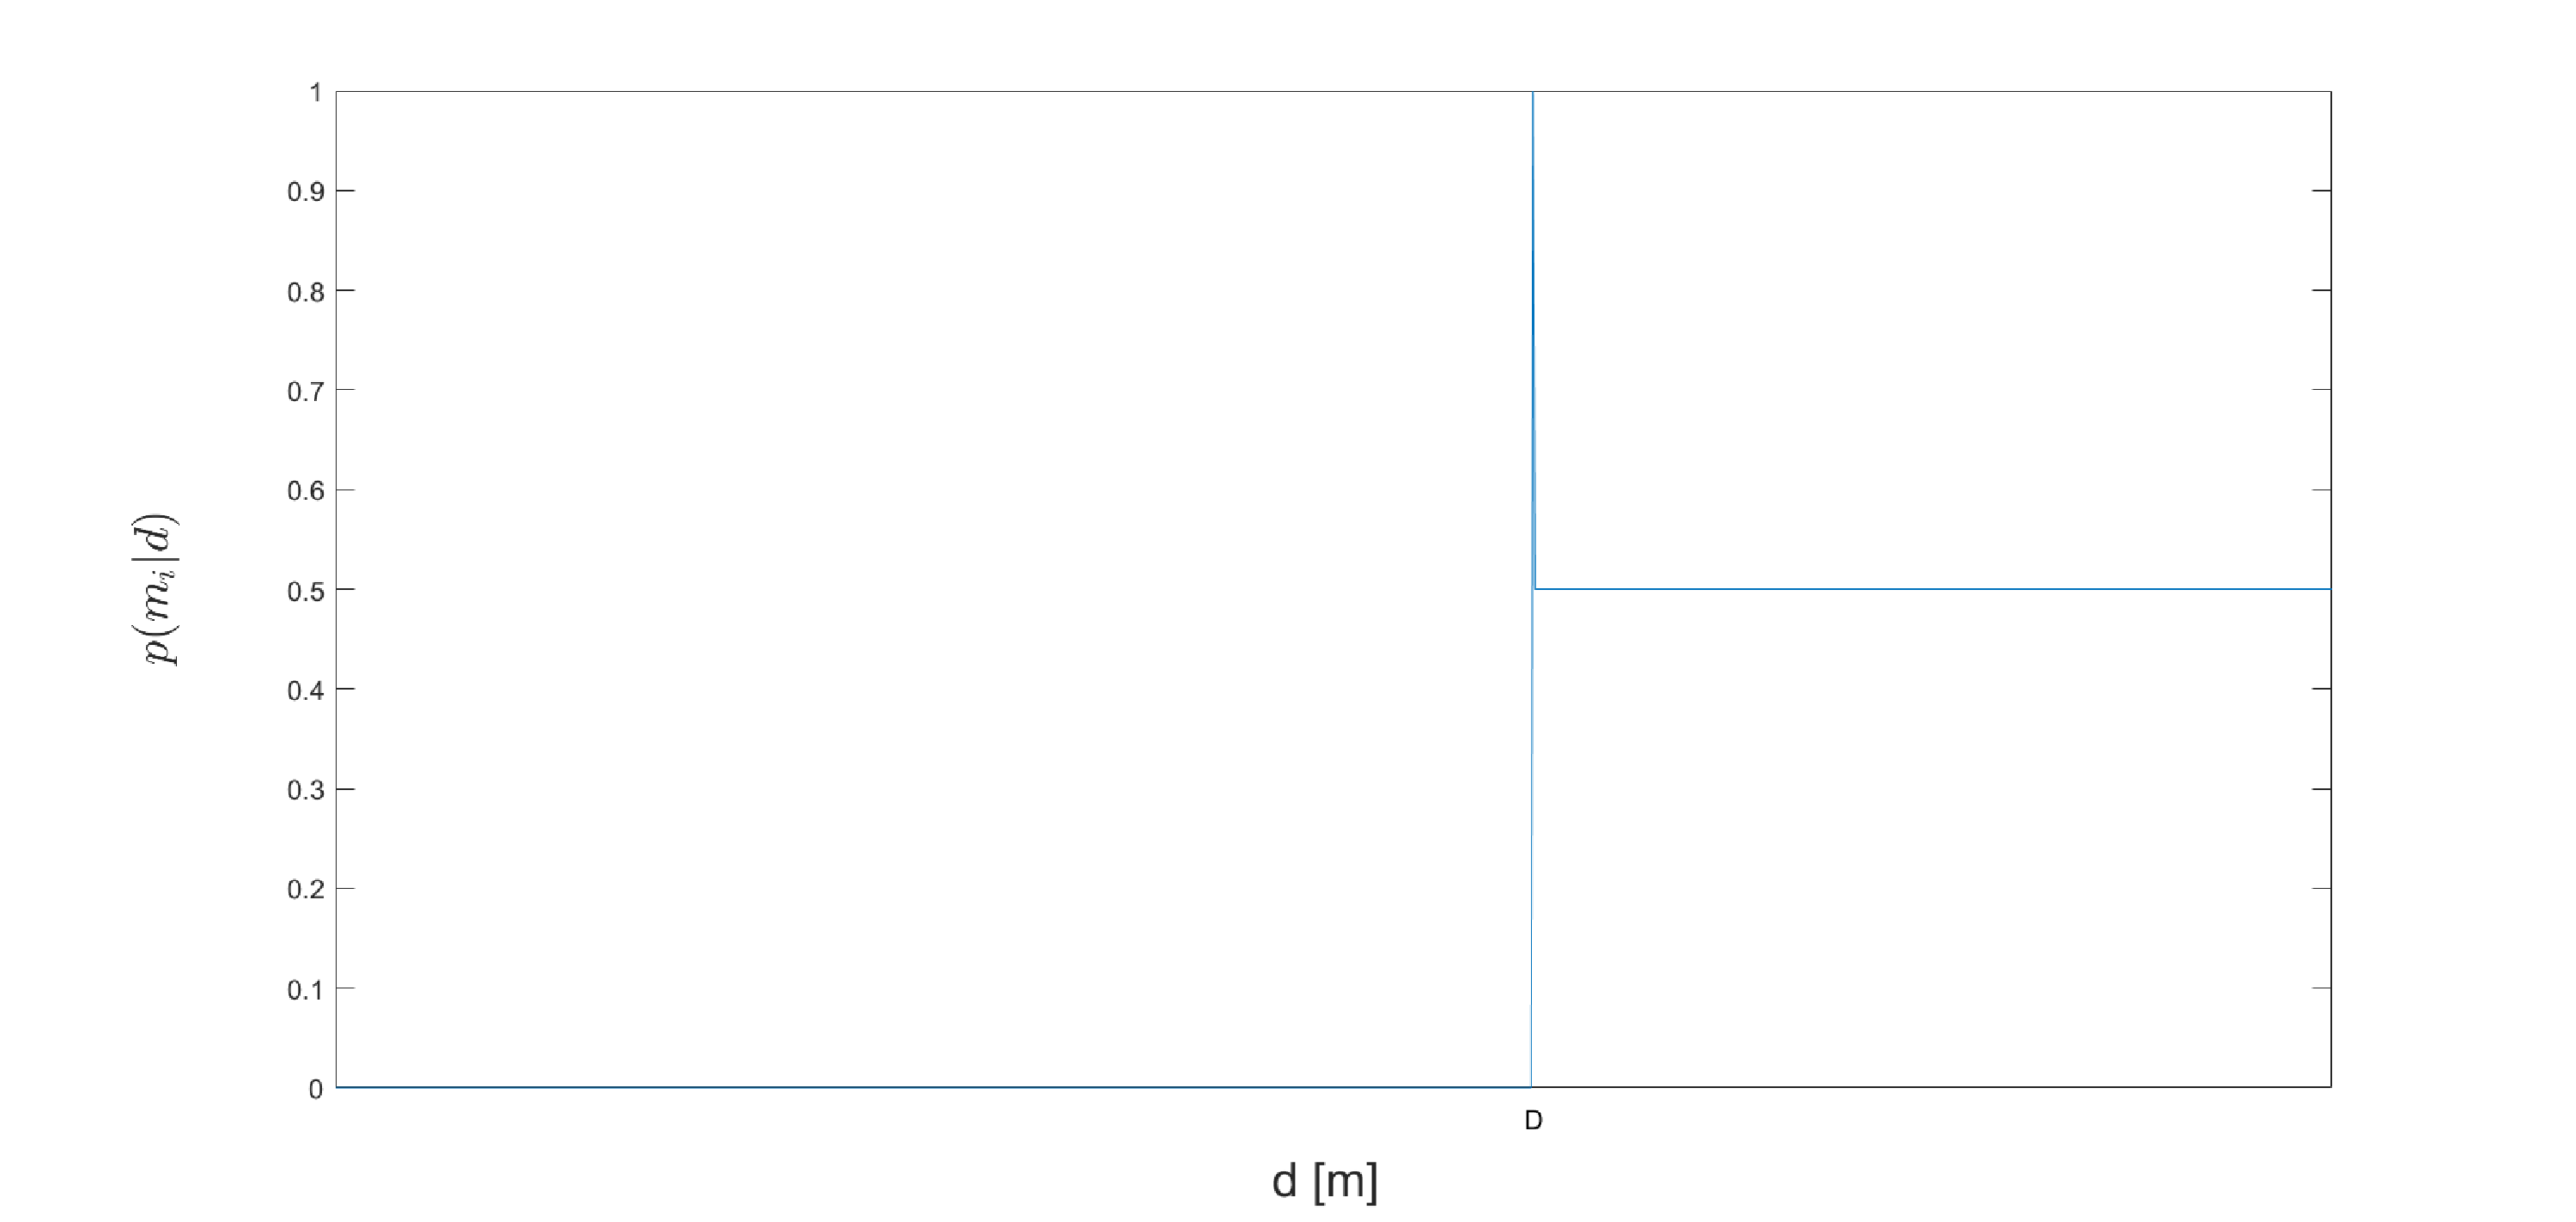
\includegraphics[width=0.8\textwidth]{pics/ideal_sensormodell.pdf}
	\caption{Das ideale Sensormodell}
	\label{fig:ideal_sensormodell}
\end{figure}
Das Diagramm veranschaulicht die ideale Zusammenhang zwischen der Belegungswahrscheinlichkeit der Zelle mit dem Index i und dem Abstand vom Laserscanner. Es ist angenommen, dass sich ein punktf�rmiges Objekt in einer Entfernung von D befindet. Ohne Messabweichung bzw. Unsicherheit besitzt das ideale Modell eine besonders einfache Funktion. Vor dem Objekt bzw. dem Hindernis ist es angenommen, dass es kein anderes Hindernis existiert. Die Wahrscheinlichkeit der Zelle, die von Laserscanner mit einem Abstand von D entfernt, betr�gt 1. Hinter dem Hindernis sind alle Zelle verborgen, weshalb die Wahrscheinlichkeit unver�ndert bleibt und als A-priori-Wahrscheinlichkeit von $0,50$ angegeben wird. 
\\Jedoch unterliegt jede Messung aus verschiedenen Gr�nden einer gewissen  Messunsicherheit~\citep{Hegerhorst.2018}, weshalb das ideale Sensormodell eine bescheidene Genauigkeit bietet. Unter Ber�cksichtigung der Messunsicherheit kann das inverses Sensormodell von ideal vereinfachend bis stark komplex sein~\citep{Pieringer.2013}. Allerdings wird die Funktion, die das inverse Sensormodell definiert, in der Praxis nach der bisherigen Erfahrungen bestimmt. Basierend auf~\citep{Weiss.1306200715062007}~\citep{Pieringer.2013}~\citep{Hegerhorst.2018} wird im Rahmen dieser Arbeit je nach Situation zwei bestimmte abschnittsweise definierte Funktionen angewendet. Die beide Funktionen weisen darauf hin, dass die Zellen innerhalb des minimalen erfassbaren Abstands mit einer niedrigen und konstanten Wahrscheinlichkeit hinzugef�gt werden. Das inverse Sensormodell ist eine Erweiterung des idealen Sensormodells, wenn ein Hindernis detektiert wird. Wie in Abbildung~\ref{fig:sesormodellmitD} dargestellt, ist der Freiraum vor dem detektierten Hindernis durch eine monoton ansteigende lineare Funktion zu beschreiben. Der Belegungswahrscheinlichkeit des als Hindernis erkannten Quadrats wird ein h�herer Wert zugewiesen, z. B. 0,9. Wie beim idealen Modell wird auch bei diesem Modell hinter dem Hindernis ein Wahrscheinlichkeitswert von 0,5 zugewiesen.
\begin{figure}[htbp]
	\centering
	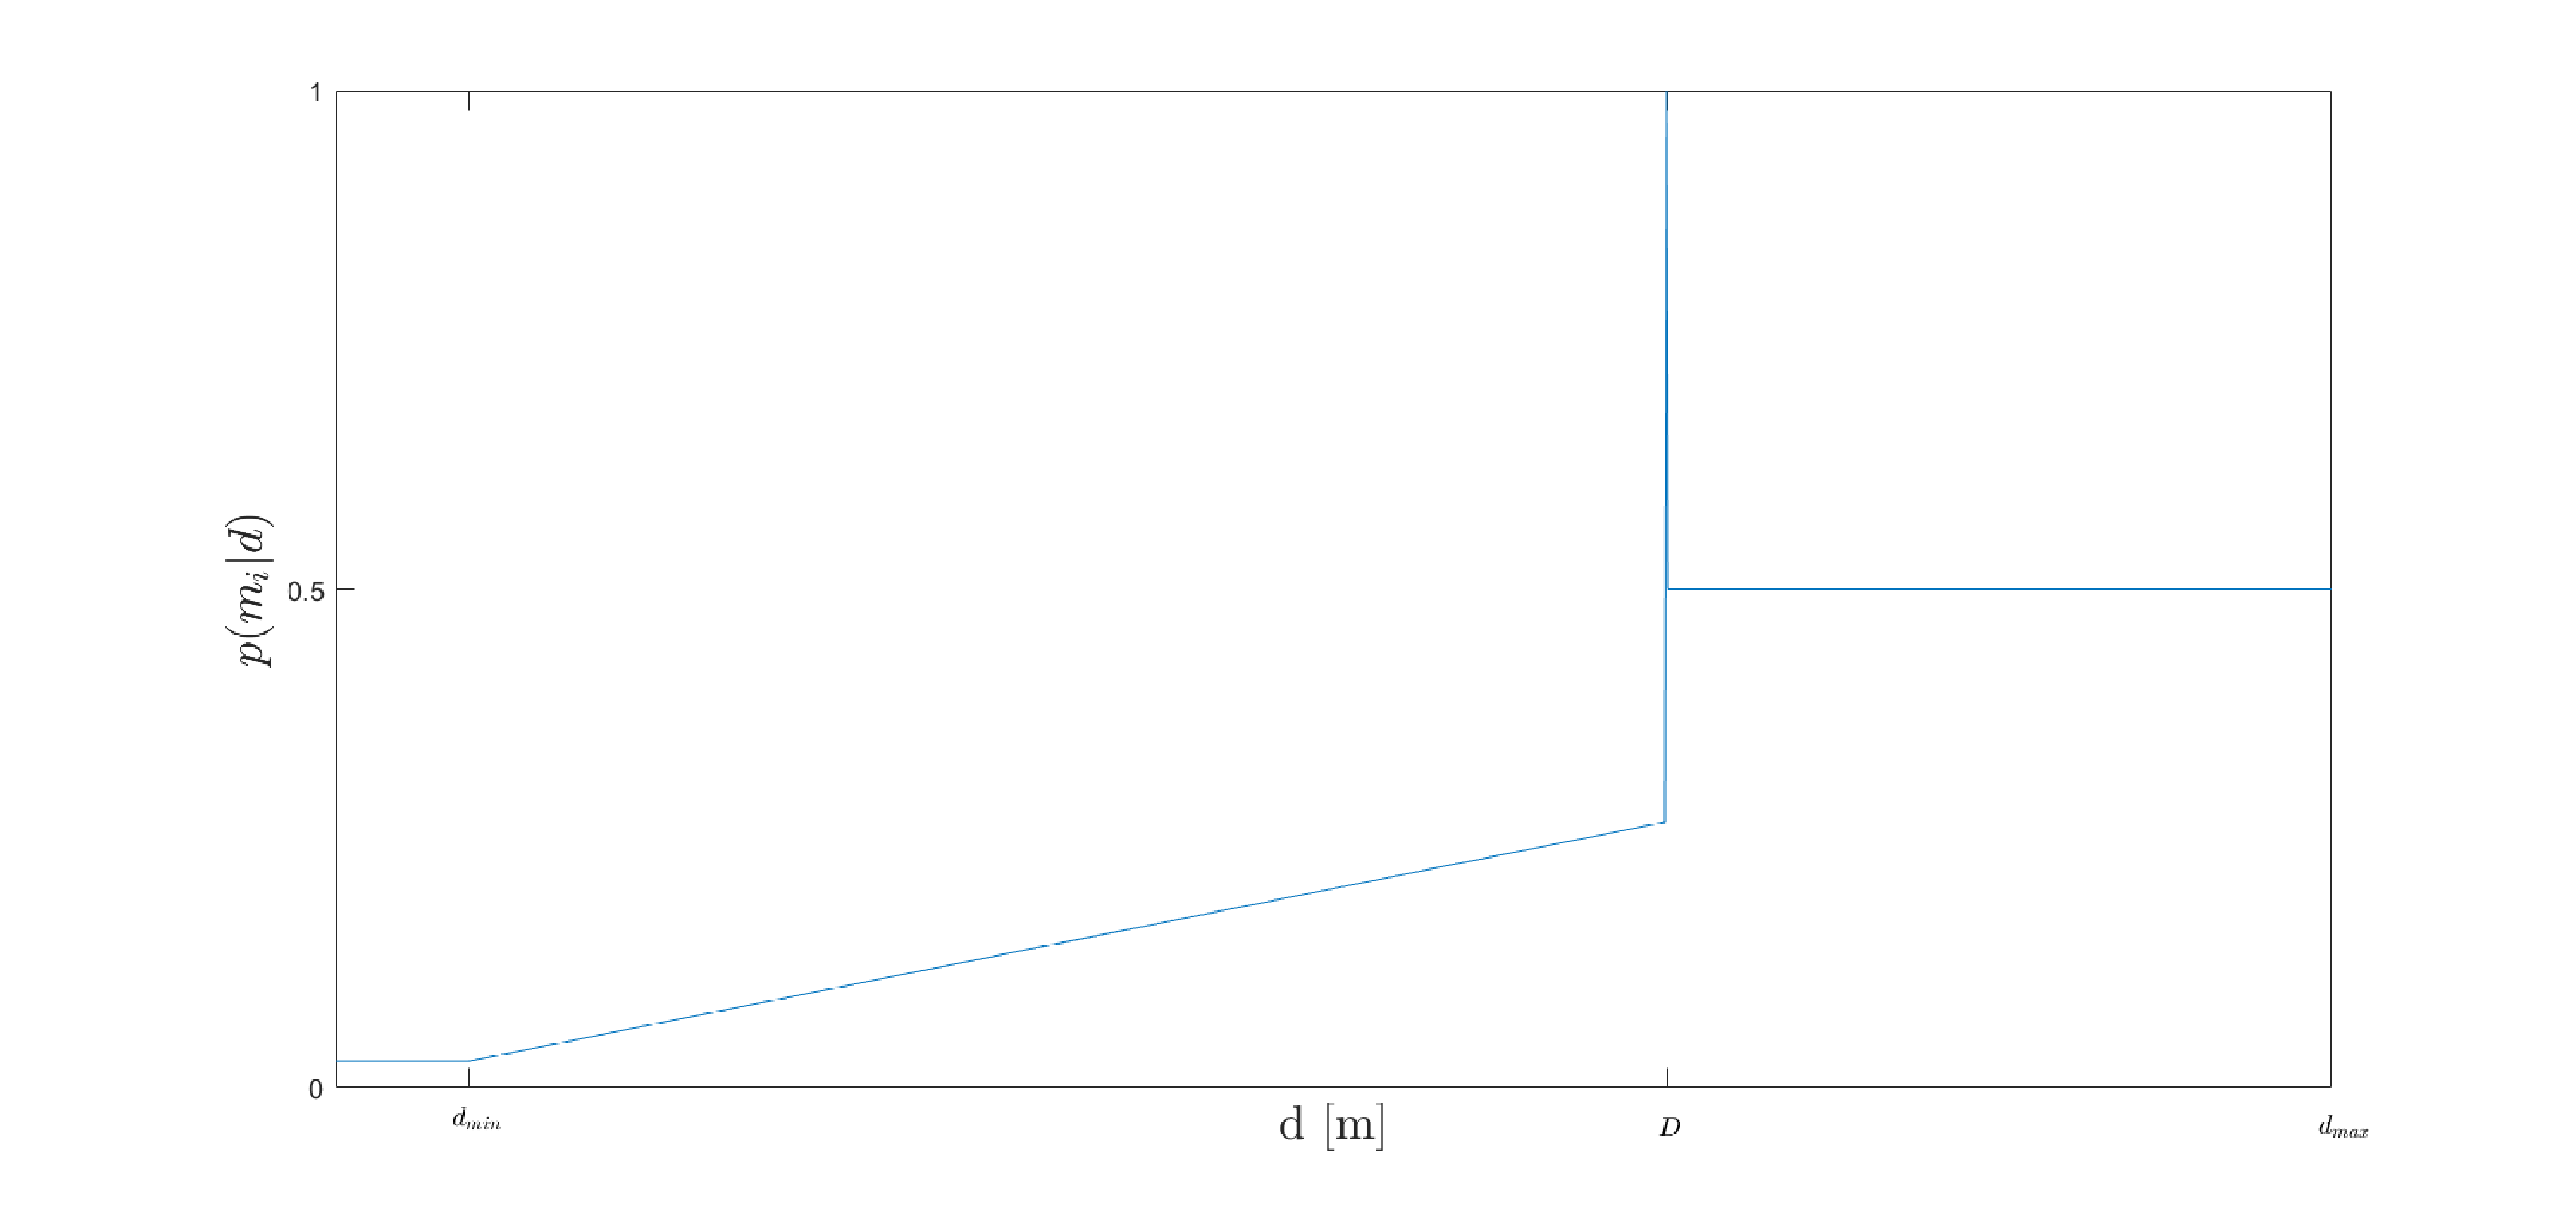
\includegraphics[width=0.8\textwidth]{pics/sesormodellmitD.pdf}
	\caption{Das inverses Sensormodell, wenn ein Hindernis detektiert wird}
	\label{fig:sesormodellmitD}
\end{figure}
Hierbei wird die mit gr��erer Entfernung entstehende Messunsicherheit abgebildet, indem die Belegungswahrscheinlichkeit mit zunehmender Distanz von dem Laserscanner erh�ht wird~\citep{Hegerhorst.2018}. Besteht kein Hindernis, wird die Funktion in die in Abbildung~\ref{fig:sesormodellohneD} gezeigte Beschreibung umgewandelt. 
\begin{figure}[htbp]
	\centering
	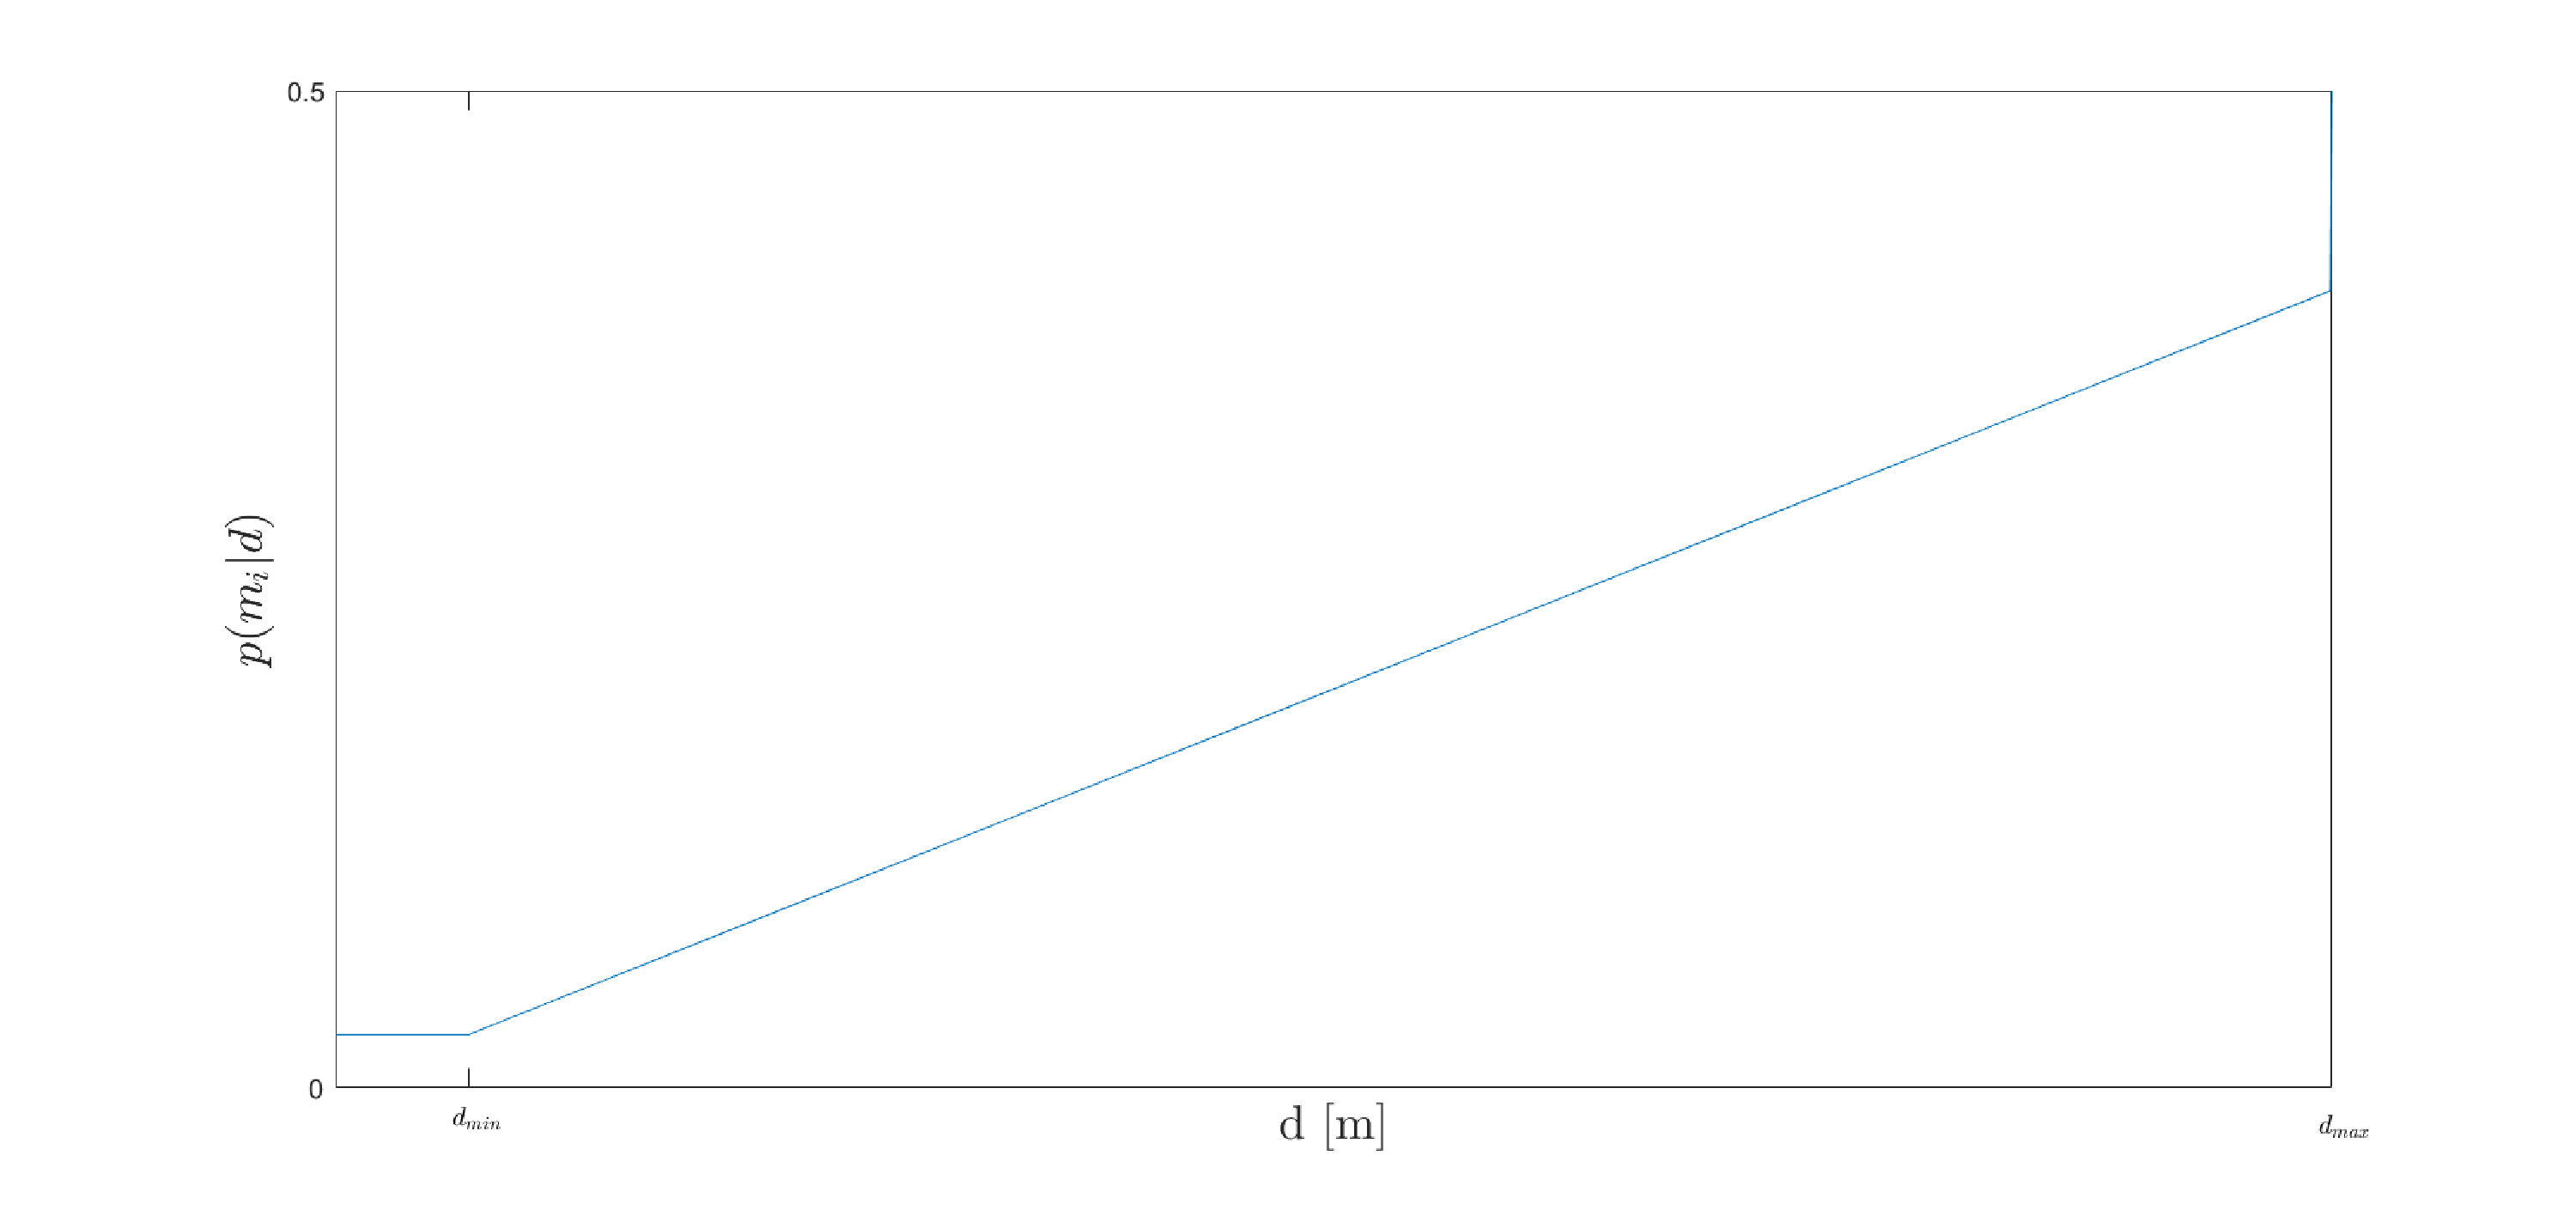
\includegraphics[width=0.8\textwidth]{pics/sesormodellohneD.pdf}
	\caption{Das inverses Sensormodell, wenn kein Hindernis detektiert wird}
	\label{fig:sesormodellohneD}
\end{figure}
In diesem Fall steigt die Wahrscheinlichkeitsfunktion im Bereich der maximalen Erfassungsentfernung und der minimalen Entfernung monoton an. Bei maximaler Entfernung steigt der Wahrscheinlichkeitswert auf 0,5.
\\Da diese Funktionen linear und einfach sind, wird die Echtzeitanforderung in gewissem Ma� gew�hrleistet. Dar�ber hinaus werden die Steigung, der minimale bzw. maximale Abstand und die Wahrscheinlichkeit der Zelle mit dem Abstand parametrisiert und  bei der folgenden Implementierung justiert. Zus�tzlich werden die Steigung, der minimale oder maximale Abstand und die Wahrscheinlichkeit der Zelle, die sich mit diesen beiden Abst�nden befindet, so parametrisiert, dass sie je nach Anwendung variieren k�nnen.

\section{Implementierung}
\label{Kapitel:Implementierung}
Basierend auf den theoretischen Grundlagen von Kapitel~\ref{Kapitel:Theoretische Grundlagen} liegt der Schwerpunkt dieses Kapitels auf der tats�chlichen Implementierung des Umfeldmodells im Ros-System. Dar�ber hinaus werden einige Features f�r die Erweiterung des System oder die Integration von anderen Funktionen hinzugef�gt.

\subsection{Versuchsfahrzeug}
Bevor mit Implementierung des in Kapitel~\ref{Kapitel:Theoretische Grundlagen} entwickelten Umfeldmodells begonnen wird, werden die relevanten Informationen �ber das Versuchsfahrzeug mitsamt die darin eingebauten Sensoren dokumentiert und in der eigentlichen Implementierung parametriert.
\subsubsection{Dimension �ber Versuchsfahrzeug}
\label{Abschnitt:DimensionVonAuto}
Bei Implementierung im Rahmen dieser Arbeit ist es auch bedeutungsvoll, die Position bzw. den belegten Raum des Versuchsfahrzeugs zu modellieren und dokumentieren, was einen konkreten Beitrag zur kollisionsfrei Navigation leistet. Au�erdem ist die Information �ber die Anordnung der Lasersensoren eng verbunden mit der Abmessung des Fahrzeugs. Daher wird die Dimension des Fahrzeugs als ein wichtiges Element betrachtet. Die Abbildung~\ref{fig:DimensionVonAuto} zeigt, dass die wichtige Gr��en von Abmessung des Fahrzeugs parametriert werden. Obwohl die Zeichnungsbema�ung eigentlich redundant ist, wird sie mit Absicht angewendet, um die Darstellung der wichtigen Gr��en sichtbar zu machen. Der Rot Punkt bezeichnet hierbei die Koordinatenursprung des Fahrzeugkoordinatensystem und befindet sich mittig auf der Hinterachse~\citep{Hegerhorst.2018}. Die X-Achse des Fahrzeugkoordinatensystem zeigt die L�ngsrichtung des Fahrzeugs nach vorne~\citep{Hegerhorst.2018}. Die Y-Achse verl�uft senkrecht zur X-Achse und zeigt nach links des Fahrtrichtung. Die Koordinatenursprung dient als ein Bezugspunkt und die Gr��en, z.B. die Lage eines Sensors sowie die Position eines detektierten Objekts, werden nur relativ zu dem Bezugssystem bzw. Fahrzeugkoordinatensystem angegeben. 
\begin{figure}[htbp]
	\centering
	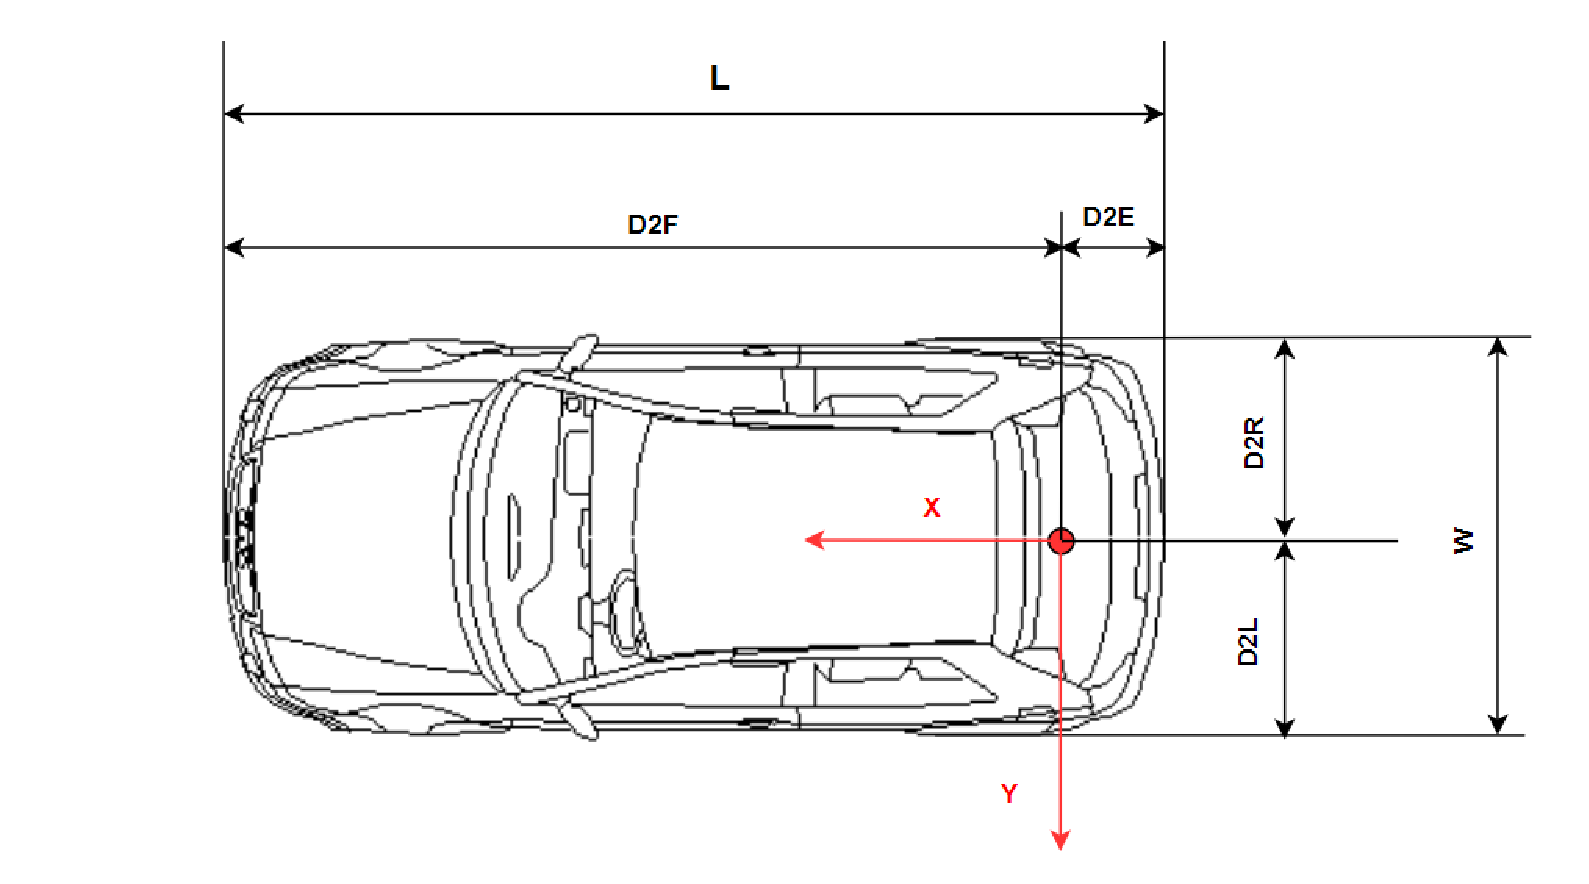
\includegraphics[width=1.0\textwidth]{pics/DimensionVonAuto.pdf}
	\caption{Dimension von Versuchsfahrzeug}
	\label{fig:DimensionVonAuto}
\end{figure}
\\In ifF stehen Golf7 (TIAMO) und Passat Alltrack (TEASY 3) als Versuchsfahrzeuge zur Verf�gung\citep{Hegerhorst.2018}. Die der Abbildung~\ref{fig:DimensionVonAuto} entsprechenden Abmessungen von diesen Versuchsfahrzeugen werden in Tabelle~\ref{tab:Abmessung von Versuchsfahrzeuge} aufgelistet.
\begin{table}[ht]
	\caption{Abmessung von Versuchsfahrzeuge}
	\label{tab:Abmessung von Versuchsfahrzeuge}
	\centering
	\begin{tabular}{|c|c|c|}
		\hline
		\textbf{Abmessung} & \textbf{Golf 7 (TIAMO)} & \textbf{Passat (TEASY 3)}\\
		\hline
		L & $4.3$ & $4.6$\\
		\hline
		W & $1.8$ & $1.6$\\
		\hline
		D2F & $3.5$ & $3.6$\\
		\hline
		D2E & $0.8$ & $1.0$\\
		\hline
		D2L & $0.9$ & $0.8$\\
		\hline
		D2R & $0.9$ & $0.8$\\
		\hline
	\end{tabular}
\end{table}
\subsubsection{Einbauposition der Ibeo-Laserscanner}
Die Anzahl und die Anordnung der im Versuchsfahrzeug installierten Ibeo-Laserscanner dienen auch als wichtigen Parametern bei Implementierung, denn diese Informationen liefern den Startpunkt des Strahls jedes Sensors. In Abbildung~\ref{fig:DimensionVonAuto} sind die Einbauposition und der Erfassungsbereich jedes Sensors dargestellt. Dazu werden die tats�chlichen Werte in Tabelle~\ref{tab:Werte der Einbauposition und des Winkels des Anfangsstrahls jedes Sensors bei TIAMO} und Tabelle~\ref{tab:Werte der Einbauposition und des Winkels des Anfangsstrahls jedes Sensors bei Passat} gegeben. In den Tabellen bezeichnet x die x-Koordinate im Fahrzeugkoordinatensystem und b die y-Koordinate. Der Winkel $\theta$ beschreibt die ausgesandte Richtung des Anfangsstrahls. Der Anfangsstrahl jedes Laserscanners ist gegen den Uhrzeigersinn zur Endstrahl. Der Winkelbereich des Erfassungsraum des Sensors ist nach der Tabelle~\ref{tab:technische Details von Ibeo LUX} auf $110^\circ$ begrenzt. Dieser Wert wird in der Praxis entsprechend der Performance des Umfeldmodells angepasst.
\begin{figure}[htbp]
	\centering
	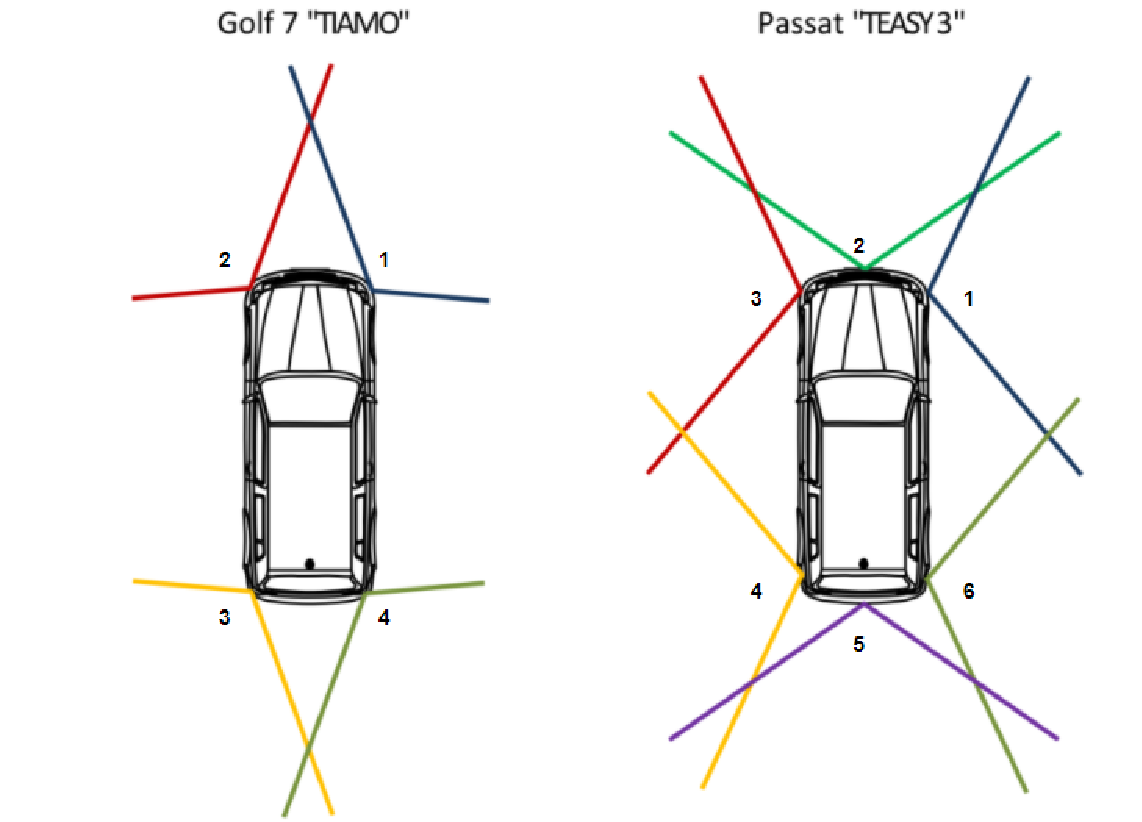
\includegraphics[width=0.7\textwidth]{pics/AnordnungDerLaserscanner.pdf}
	\caption{Einbauposition und Erfassungsbereich der Ibeo-Laserscanner}
	\label{fig:AnordnungDerLaserscanner}
\end{figure}
\begin{table}[ht]
	\caption{Werte der Einbauposition und des Winkels des Anfangsstrahls jedes Sensors bei Golf 7 (TIAMO))}
	\label{tab:Werte der Einbauposition und des Winkels des Anfangsstrahls jedes Sensors bei TIAMO}
	\centering
	\begin{tabular}{|c|c|c|c|}
		\hline
		\textbf{Sensor ID} & \textbf{x (m)} & \textbf{y (m)} & \textbf{Winkel $\theta$ des Anfangsstrahls ($^\circ$)}\\
		\hline
		1 & $3$ & $-0.9$ & $-10$\\
		\hline
		2 & $3$ & $0.9$ & $80$\\
		\hline
		3 & $-0.7$ & $0.9$ & $170$\\
		\hline
		4 & $-0.7$ & $-0.9$ & $-100$\\
		\hline
	\end{tabular}
\end{table}
\begin{table}[ht]
	\caption{Werte der Einbauposition und des Winkels des Anfangsstrahls jedes Sensors bei Passat (TEASY 3)}
	\label{tab:Werte der Einbauposition und des Winkels des Anfangsstrahls jedes Sensors bei Passat}
	\centering
	\begin{tabular}{|c|c|c|c|}
		\hline
		\textbf{Sensor ID} & \textbf{x (m)} & \textbf{y (m)} & \textbf{Winkel $\theta$ des Anfangsstrahls ($^\circ$)}\\
		\hline
		1 & $3.3$ & $-0.8$ & $-35$\\
		\hline
		2 & $3.6$ & $0$ & $45$\\
		\hline
		3 & $3.3$ & $0.8$ & $125$\\
		\hline
		4 & $-0.5$ & $0.8$ & $145$\\
		\hline
		5 & $-1$ & $0$ & $-135$\\
		\hline
		6 & $-0.5$ & $-0.8$ & $-55$\\
		\hline
	\end{tabular}
\end{table}
\subsection{Framework ROS zur Implementierung}
Eine der zentralen Aufgaben dieser Arbeit handelt sich um die Konvertierung von dem am IfF bereits bestehenden MATLAB/Simulink-Modell nach Robot Operating System (ROS).Das Robot Operating System (ROS) ist ein Framework zum Schreiben von Robotersoftware. Es handelt sich um eine Sammlung von Tools, Bibliotheken und Konventionen, die darauf abzielen, die Erstellung komplexer und robuster Roboterverhalten auf einer Vielzahl von Roboterplattformen zu vereinfachen\citep{Quigley.2015}. Obwohl diese Idee aus dem Bereich der Robotik stammt, machen ihre verschiedenen guten Eigenschaften ihre Investition in den Bereich des autonomen Fahrens sehr bedeutsam. Um eine klare Programmstruktur und eine genaue und effiziente Umsetzung des in Kapitel~\ref{Kapitel:Theoretische Grundlagen} genannten Umfeldmodells zu erhalten, ist eine kurze Einf�hrung in die ROS-Grundlagen und Funktionsmodule in Bezug auf diesen Artikel erforderlich.
\subsubsection{Grundlagen der ROS-Architektur}
Die ROS-Architektur, die in Abbildung~\ref{fig:ROS-Architektur} dargestellt, wurde entworfen und in drei Abschnitte oder Konzeptebenen unterteilt, welche sich um die Dateisystemebene (engl. The Filesystem level), die Berechnungsdiagrammebene (engl. The Computation Graph level) und die Community-Ebene (engl. The Community level) handeln~\citep{Fernandez.2015}.
\begin{figure}[htbp]
	\centering
	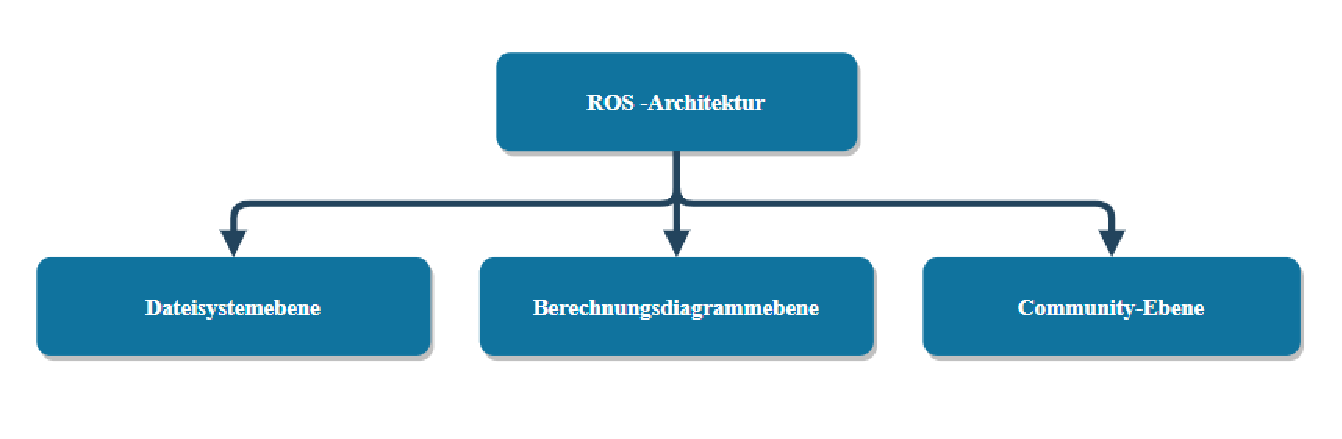
\includegraphics[width=1.0\textwidth]{pics/ROS-Architektur.pdf}
	\caption{ROS-Architektur}
	\label{fig:ROS-Architektur}
\end{figure}
\\Auf der Dateisystemebene wird eine Gruppe von Konzepten verwendet, um zu erkl�ren, wie ROS intern gebildet wird. �hnlich wie bei einem Betriebssystem ist ein ROS-Programm in Ordner unterteilt, und diese Ordner enthalten Dateien, die ihre Funktionen beschreiben~\citep{Fernandez.2015}. Hierbei sind die wichtigen Konzepte zu diesem Artikel Package und Metapackage. Das Package ist die zentrale und grundlegende Dateiorganisationseinheit, die Programmierfunktionen in ROS vollst�ndig realisieren kann. Es enth�lt im Allgemeinen ROS Laufzeitprozess (engl. runtime process), Quellcode (engl. Sourcecode), Konfigurationsdateien (engl. configuration files) und das Package-manifest, das zur Bereitstellung von Informationen von build-dependencies, run-dependencies und Lizenz verwendet wird. Metapackages werden in der Regel nach einer �hnlichen Funktionalit�t gruppiert. Andere Grundkonzepte und Begriffe auf dieser Ebene sind aufgrund der L�nge des Artikels nicht detailliert und finden sich in~\citep{Fernandez.2015}\citep{Koubaa.2016}.
\\Die Berechnungsdiagrammebene ist die relevanteste Ebene f�r diese Arbeit, auf der die Kommunikation zwischen Prozessen und Systemen stattfindet. Die Grundkonzepte auf dieser Ebene sind, wie in Abbildung~\ref{fig:Berechnungsdiagrammebene} dargestellt, Nodes, ROS-Master, Parameter Server, Messages, Topics, Services und ROS-Bags, die alle Daten auf unterschiedliche Weise f�r das Diagramm bereitstellen~\citep{Fernandez.2015}.
\begin{figure}[htbp]
	\centering
	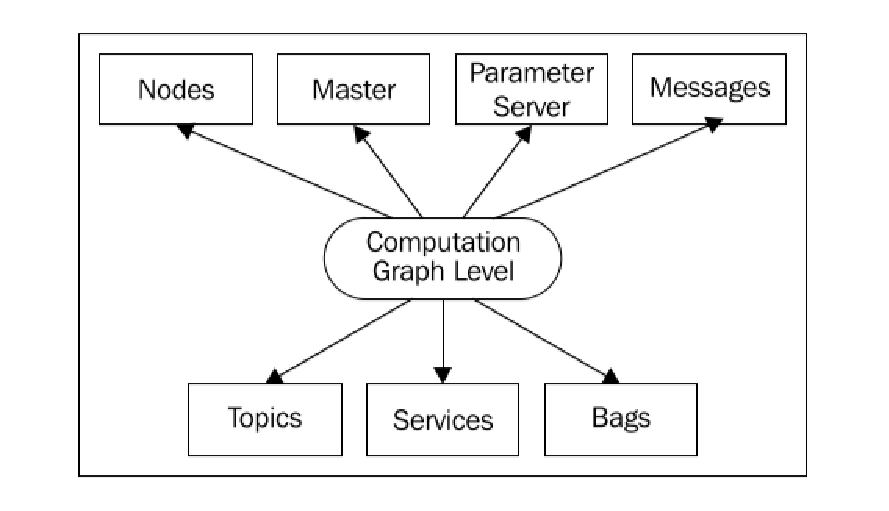
\includegraphics[width=0.7\textwidth]{pics/Berechnungsdiagrammebene.pdf}
	\caption{Wesentliche Grundkonzepte von Berechnungsdiagrammebene}
	\label{fig:Berechnungsdiagrammebene}
\end{figure}
Nodes sind ausf�hrbare Dateien (engl. executables) in ROS und vervollst�ndigen die erwartete Funktion und die zugeh�rigen Berechnungen. Die Nodes k�nnen miteinander kommunizieren und Daten �bertragen. Daher gibt es im Allgemeinen mehrere Nodes in einem System, die unterschiedliche Funktionen ausgef�hrt haben. Der Datenaustausch zwischen Nodes erfolgt �ber Messages. ROS verwendet eine vereinfachte Nachrichtenbeschreibungssprache, um die Datenwerte zu beschreiben, die von Nodes publiziert (engl. published)~\citep{Fernandez.2015}. Damit kann ROS den richtigen Quellcode f�r diese Nachrichtentypen in mehreren Programmiersprachen (z.B. C++ oder Python) generieren. Zahlreiche vordefinierte Messages in ROS k�nnen direkt zum �bertragen von Daten oder zum Erstellen neuer aufgabenorientierter Messages verwendet werden. Dies erfolgt durch Definieren einer Datei mit .msg-Extension. Wenn ein Node Daten sendet, hei�t es, dass das Note eine Topic publizieren. Ein anderer Knoten kann die Topic abonnieren (engl. subscribe), um die Daten abzurufen. Ein Node kann eine Topic nur abonnieren, wenn es denselben Message-Typ hat. Eine Topic kann verschiedene Subsribers und auch verschiedene Publishers haben. Wenn die Kommunikation zwischen Nodes empfangen und beantwortet (engl. receive and reply) werden muss, sollten Services anstelle von Topics verwendet werden. Services geben den Entwicklern die M�glichkeit, mit Nodes zu interagieren. Mit Parameter Server ist es m�glich, Schl�ssel zu verwenden, um Daten an einem zentralen Ort zu speichern und Nodes w�hrend der Ausf�hrung zu konfigurieren oder die Nodes der Knoten zu �ndern~\citep{Fernandez.2015}. Die oben genannte Kommunikation garantiert ROS-Master, der jede Nodes verwalten. Nodes werden zuerst beim Master registriert, und dann integriert der Master Nodes in das gesamte ROS-Programm. Auf diesem Grund besteht der erste Schritt darin, den Master zu starten, wenn das ROS-Programm gestartet wird. ROS-Bag ist ein Format zum Speichern und Wiedergeben aller Informationen der Messages, Topics und Services, die gew�nscht werden. In dieser Arbeit wird ROS-Bag verwendet, um die Sensordaten von dem Versuchsfahrzeug zu speichern. Wenn das ROS-Bag wiedergegeben ist, simuliert es die Datenwerte von Sensoren zu messen und erfassen, was ist praktisch zum Debuggen von Implementierungsalgorithmus.
\\Die Konzepte auf ROS-Community-Ebene sind die ROS-Ressourcen, die es separaten Communities erm�glichen, Software und Wissen auszutauschen~\citep{Fernandez.2015}. Zu den Ressourcen geh�ren unter anderem ROS-Repositories,ROS-Distributions und ROS-Wiki. Jedoch hat diese Ebene f�r diesen Artikel nur eine sehr geringe Relevanz. Auf diesem Grund ist die Auseinandersetzung damit im Rahmen dieser Arbeit zu verzichten.
\\Aufgrund des oben erw�hnten Mechanismus und der Philosophie von ROS hat der Aufbau der Implementierung des Umfeldmodell auf ROS einen starken Vorteil. Die dezentrale Kommunikationsmethode macht das Implementierungssystem klarer und einfacher. Au�erdem sind Fehler im System leichter zu finden und sortieren. Die Aufteilung zwischen verschiedenen Funktionen erleichtert die sp�tere Systemerweiterung, z.B. Navigation bzw. kollisionsfreie Pfadplanung. Im Rahmen dieser Arbeit ist f�r die Implementierung ROS-Kinetic-Kame mit Ubuntu 16.04 (Xenial) in Benutzung.
\subsubsection{Visualisierung des Umfeldmodells in ROS}
\label{Visualisierung des Umfeldmodells in ROS}
Die Visualisierung des Modells ist ebenso wichtig wie seine Einrichtung und Implementierung. Eine gute Visualisierung spiegelt den tats�chlichen Betriebsstatus des Modells hervorragend wider. Dies hilft bei der Behebung von Programmfehlern und beim Datenaustausch mit anderen Funktionsmodulen oder Modellen im nachfolgenden Systemerweiterungsprozess. Das ROS-System bietet eine Vielzahl von Tools zur Datenvisualisierung und zum Debuggen. Das wichtigste und am weitesten verbreitete ist RVIZ. rviz ist ein 3D-Visualisierungswerkzeug von ROS, mit dem Sensordaten und Statusinformationen visualisiert werden. RVIZ unterst�tzt umfangreiche Datentypen, die durch Laden verschiedener Display-Typen visualisiert werden. Jeder Display hat einen eindeutigen Namen. Wichtige Display-Typen und ihre entsprechenden Message-Typen im Bereich des autonomen Fahrens sind in Tabelle~\ref{tab:RVIZ Display-Typen} aufgef�hrt. Aufgrund der Philosophie des verteilten Software-Frameworks von ROS muss das RVIZ-Visualisierungstool nur den passenden Message-Typ und die passende Topic ausw�hlen, wenn Daten auf einer Topic visualisiert werden sollen.
\begin{table}[ht]
	\caption{Display-Typen und ihre entsprechenden Message-Typen in RVIZ}
	\label{tab:RVIZ Display-Typen}
	\small
	\centering
	\setlength\tabcolsep{2pt}
	\begin{tabular}{|c|c|c|}
		
		\hline
		\textbf{Display-Typ} & \textbf{Message-Typ} & \textbf{Beschreibung}\\
		\hline
		Grid Cells & nav\_msgs/GridCells & Zeichnet Zellen aus einem Raster\\
		\hline
		Point Cloud 2 & sensor\_msgs/PointCloud2 & Zeigt Daten aus einer Punktwolke\\
		\hline
		Map & nav\_msgs/OccupancyGrid & Zeigt eine Karte in der Grundebene\\
		\hline
		Path & nav\_msgs/Path & Zeigt einen Pfad\\
		\hline
		Pose & geometry\_msgs/PoseStamped & Zeichnet eine 3D-Pose\\
		\hline
		Pose Array & geometry\_msgs/PoseArray & Zeichnet mehrere Posen\\
		\hline
		Image & sensor\_msgs/Image & Erstellt ein neues Rendering-Bild\\
		\hline
		Laser Scan & sensor\_msgs/LaserScan & Zeigt Daten von einem Laserscan\\
		\hline
		Odometry & nav\_msgs/Odometry & Sammelt Kilometerz�hler-Posen aus der Zeit\\
		\hline
		TF & tf2\_msgs/TFMessage & Zeigt die Koordinatentransformationshierarchie \\
		\hline
	\end{tabular}
\end{table}
\\F�r das auf diesen Artikel bezogene Umgebungsmodell gibt es zwei grundlegende Visualisierungsoptionen. Zum einen ist Display-Typ Map, das nav\_msgs/OccupancyGrid message anzeigt. Die Informationen in nav\_msgs/OccupancyGrid umfassen die Koordinaten des urspr�nglichen Standorts, die Aufl�sung sowie die L�nge und Breite der Karte und die Kartendaten (engl. Map data) in jeder Gitterzelle. Map data werden in zwei Situationen betrachtet. Einer ist, dass der Belegungszustand unbekannt ist und der Wert in diesem Fall -1 ist. Die andere ist, dass die Wahrscheinlichkeit der Belegung bekannt ist und der Wert in diesem Fall 0 bis 100 betr�gt. Wie in Abbildung~\ref{fig:Display_Map} gezeigt, wenn Map value von einer Gitterzelle -1 ist, wird die Zellenfl�che ausgegraut dargestellt. Wenn Map Value von 0 auf 100 steigt, ver�ndert sich die entsprechende Zelle in einem Farbverlauf von Wei� zu Schwarz.
\begin{figure}[htbp]
	\centering
	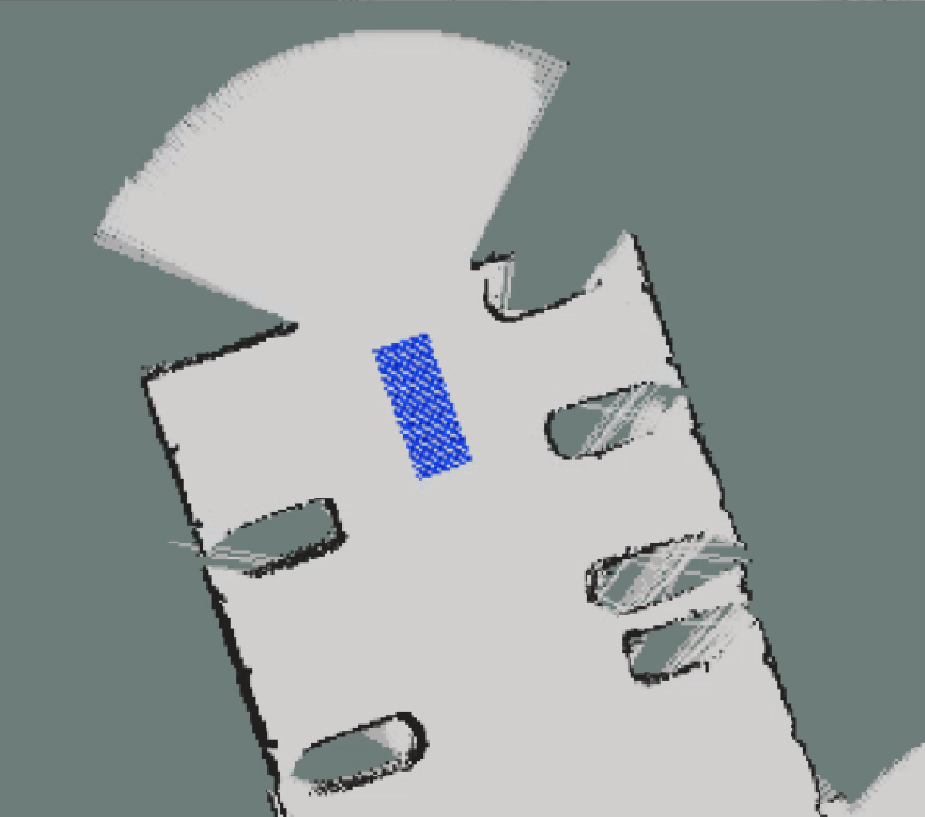
\includegraphics[width=0.5\textwidth]{pics/Display_Map.pdf}
	\caption{Display mit Map}
	\label{fig:Display_Map}
\end{figure}
\\Die zweite M�glichkeit der Visualisierung eines Umfeldmodells in RVIZ ist die Verwendung von GridCells. Dies darstellt die Daten von Message-Typ nav\_msgs/GridCells. Darin handelt sich um die Informationen �ber die L�nge und Breite sowie die Koordinaten jeder Zelle. GridCells-Display ist nur f�r die Visualisierung des vom Entwickler angegebenen Bereichs verantwortlich. Es ist von der Belegungswahrscheinlichkeit getrennt und wird einfach, leicht und flexibel. Je nach Aufgabe des Entwicklers oder Debugging-Anforderungen k�nnen unterschiedliche Wahrscheinlichkeitsbereiche angezeigt werden. Dar�ber hinaus erm�glicht es einen starken Kontrast von Farben mit unterschiedlichen Belegungswahrscheinlichkeiten. Im Gegensatz dazu ist die Graustufendarstellung von dem oben erw�hnten Map nicht offensichtlich und f�r die Programmentwicklung und die Erkennung der Datenkorrektheit nicht geeignet. Ein Anwendungsbeispiel besteht darin, wie in Abbildung~\ref{fig:Display_GridCell} gezeigt, Gitterzellen mit unterschiedlichen Belegungswahrscheinlichkeiten in verschiedenen Topics zu organisieren und dann die verschiedenen Topics mit verschiedenen offensichtlichen Farben zu visualisieren. 
\begin{figure}[htbp]
	\centering
	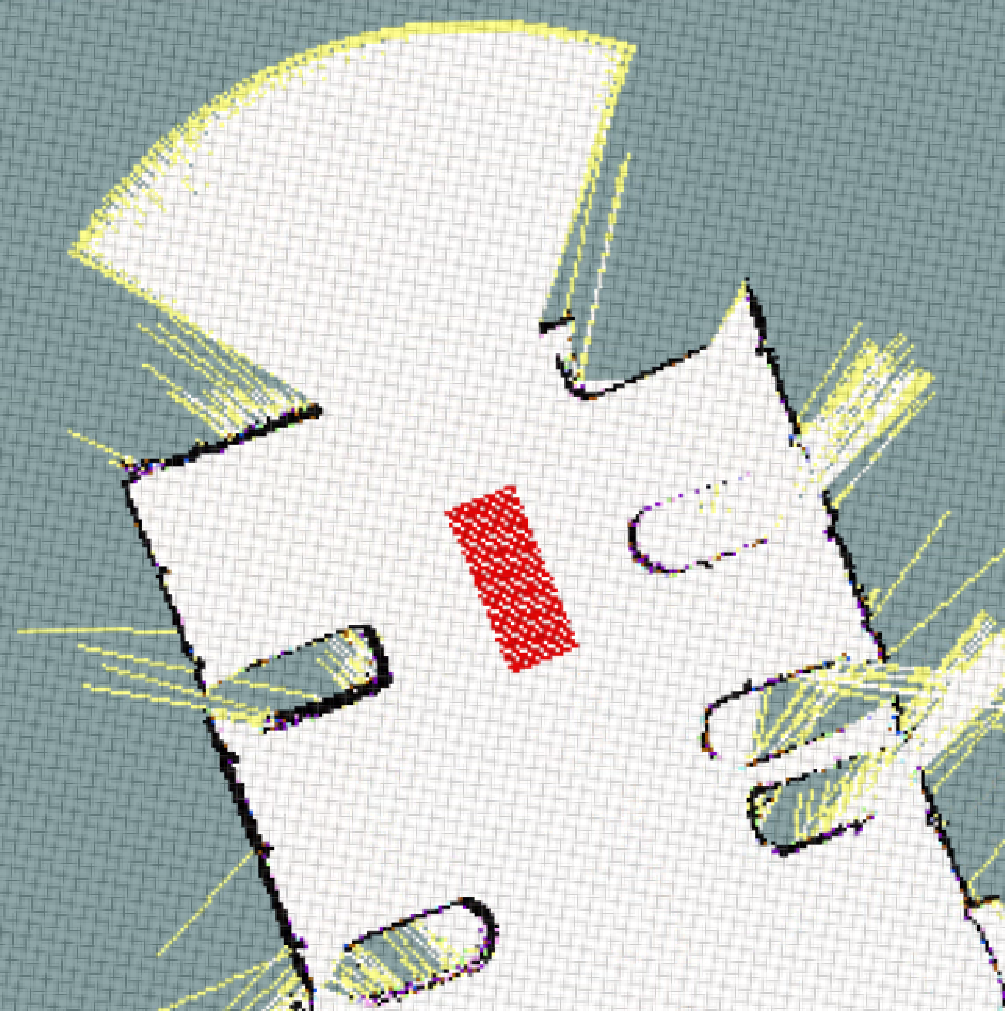
\includegraphics[width=0.5\textwidth]{pics/Display_GridCell.pdf}
	\caption{Display mit GridCell}
	\label{fig:Display_GridCell}
\end{figure}
Neben der Flexibilit�t bietet GridCells-Display einige gute Vorteile gegen�ber Map-Display. Zun�chst kann die jeder Gitterzelle zugewiesenen zus�tzlichen Informationstypen und -werten selbst definiert werden, was eine direktere Bedingung f�r die zuk�nftige Erweiterung und Verbesserung des Modells darstellt. Selbst wenn nur die Belegungswahrscheinlichkeit zu ber�cksichtigen ist, kann die Wahrscheinlichkeit (0 bis 100) als Ganzes betrachtet werden, anstatt den Wert -1 allein zu verwenden bzw. umrechnen, um das Unbekannte auszudr�cken. Dar�ber hinaus erleichtert die Verwendung von GridCells-Display die anschlie�ende Bin�risierung von Werten und Bildern. Wie in Abbildung~\ref{fig:Dispaly_Grid_Cell_Binary} gezeigt, kann die Bin�risierung durch Einstellen des Schwellenwerts, der durch Experimente oder Deep-Learning erhalten wurde, leicht erzielt werden. 
\begin{figure}[htbp]
	\centering
	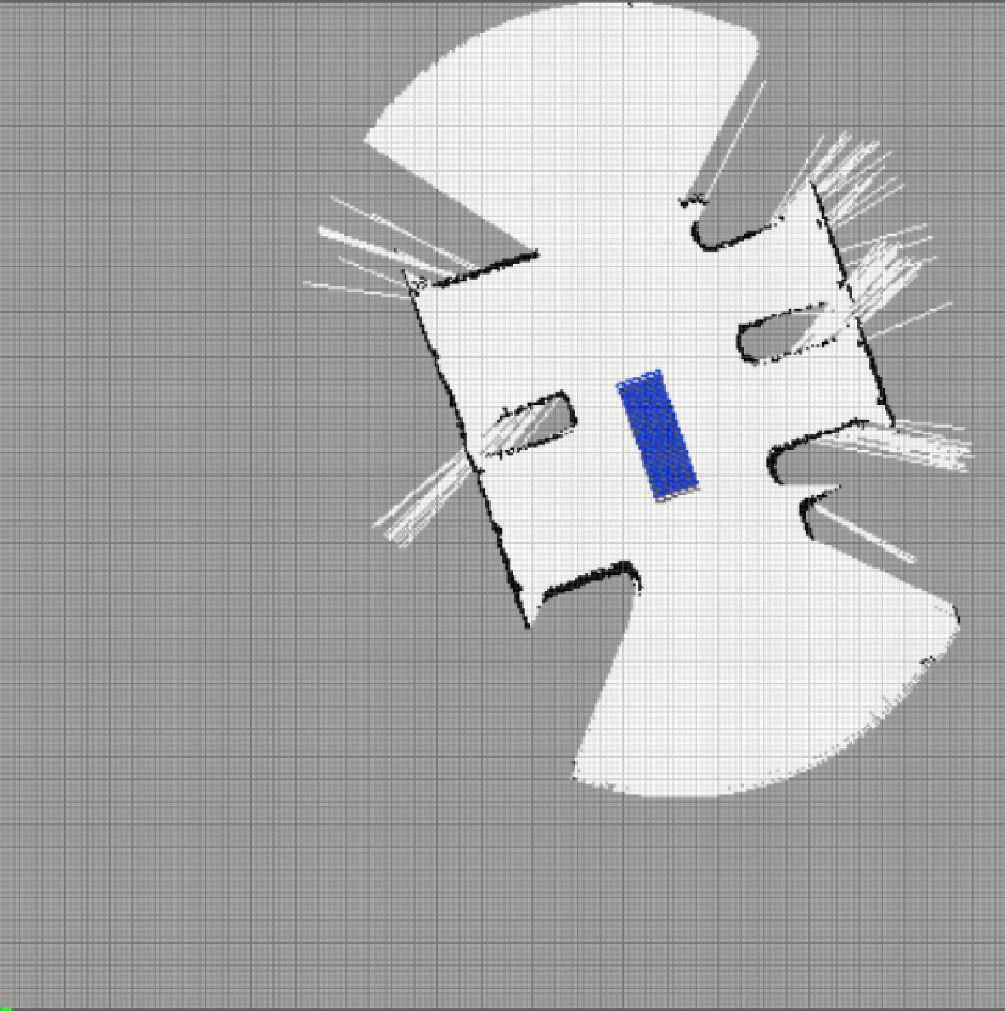
\includegraphics[width=0.5\textwidth]{pics/Dispaly_Grid_Cell_Binary.pdf}
	\caption{Display mit GridCell nach Bin�risierung}
	\label{fig:Dispaly_Grid_Cell_Binary}
\end{figure}
Daher im Rahmen dieser Arbeit wird GridCells-Display verwendet, um eine Visualisierung zu erreichen. Es gibt aber ein kleines Problem, das bei der Verwendung von GridCells besondere Aufmerksamkeit und L�sung erfordert. Durch tats�chliche Experimente ist bekannt, dass bei sehr gro�en Positionskoordinaten von GridCells (z. B. 10 bis 6 Potenzen) die Darstellung von Gitterzellen in RVIZ deformiert wird oder sogar verschwindt. Daher k�nnen bei der Implementierung des Modells die vom GPS erhaltenen UTM-Koordinateninformationen nicht direkt als Koordinaten f�r die Anzeige der Gitterzellen verwendet werden. Vor der eigentlichen Visualisierung werden zwei Abweichungen X\_VISUAL\_OFFSET und Y\_VISUAL\_OFFSET so eingestellt, dass der Koordinatenwert der Zellen nahe am Ursprung liegt, wodurch die Genauigkeit der Visualisierung sichergestellt wird. Dieses Abweichungspaar wird durch die anf�nglichen Fahrzeugkoordinateninformationen bestimmt, die bei der Initialisierung des Modells erhalten werden, was sich in der n�chsten Erl�uterung des Funktionsblocks widerspiegelt.

\subsection{Koordinatensysteme}
Daten von verschiedenen Informationsquellen bzw. Sensoren sind h�ufig mittels unterschiedlichen Koordinatensystemen gegeben. Auf diesem Grund wird die Konvertierung zwischen verschiedenen Koordinatensystemen bei der Realisierung des Umfeldmodells oft durchgef�hrt. Hierbei gibt es 3 wesentliche Koordinatensysteme, deren Kl�rung f�r das Verst�ndnis der nachfolgenden Funktionsbausteine dieser Arbeit sehr hilfreich ist. Wie in Abbildung~\ref{fig:Koordinaten3} gezeigt, sind diese 3 Koordinatensysteme Weltkoordinatensystem (engl. Global Coordinate System, als GCS abgek�rzt), Ankerkoordinatensystem (engl. Anchor Coordinate System, als ACS abgek�rzt) und Fahrzeugkoordinatensystem (engl. Vehicle Coordinate System, als ACS abgek�rzt).
\begin{figure}[htbp]
	\centering
	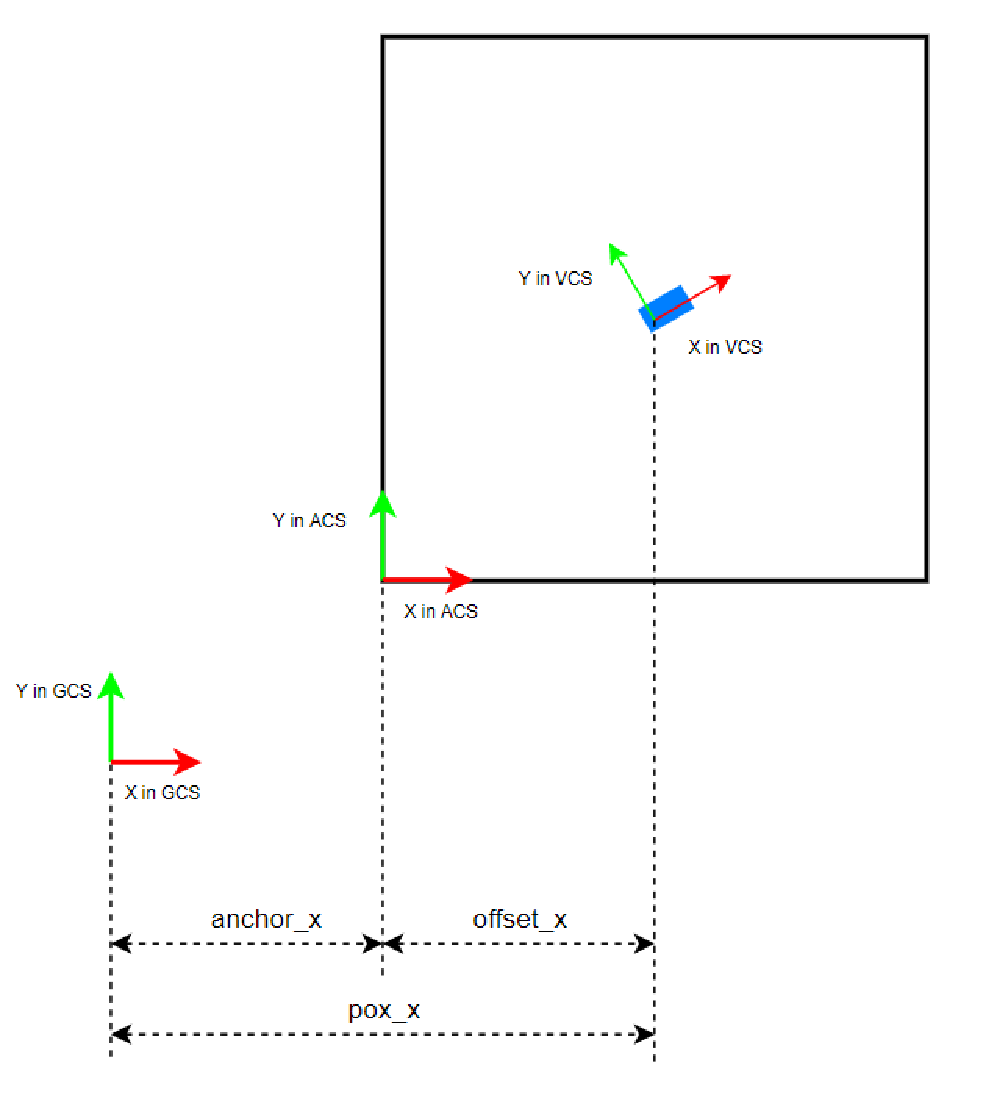
\includegraphics[width=0.7\textwidth]{pics/Koordinaten3.pdf}
	\caption{3 wesentliche Koordinatensysteme im Umfeldmodell}
	\label{fig:Koordinaten3}
\end{figure}
\subsubsection{Global Coordinate System (GCS)}
\label{Abschnitt:GCS}
Das Weltkoordinatensystem ist das grundlegendste Koordinatensystem. Die vom GPS-Sensor erhaltenen Informationen zur Fahrzeugpose basieren auf dem Weltkoordinatensystem. Im tats�chlichen Gebrauch sind daf�r zwei Umrechnungen erforderlich. Das erste ist die Notwendigkeit, die Abweichung zwischen dem Ursprung des Fahrzeugkoordinatensystems (der Mitte der Hinterachse des Fahrzeugs) und dem tats�chlichen Standort der GPS-Antenne (einer bestimmten Position auf dem Dach) zu kompensieren. Au�erdem ist die Beschreibung bzw. die Berechnung der geographischen Koordinaten mittels UTM-Koordinatensystem (von englisch Universal Transverse Mercator coordinate system) notwendig. Diese beiden Berechnungen werden nach~\citep{Hegerhorst.2018} im Vorverarbeitungsprozess unter Verwendung einiger Algorithmen von ifF abgeschlossen und werden hier nicht ausf�hrlich erl�utert. Au�erdem ist das UTM-Koordinatensystem tats�chlich  ein nordweisendes, rechtsdrehendes Koordinatensystem. Jedoch wird naher in Abschnitt~\ref{Abschnitt:GPS-Information} in ein gebr�uchliches, linksdrehendes Koordinatensystem umgerechnet. Im Rahmen dieser Arbeit beziehen sich die Koordinaten im Weltkoordinatensystem auf die verarbeitete bzw. umgerechnete  UTM-Koordinateninformationen.
\subsubsection{Vehicle Coordinate System (VCS)}
In Abbildung~\ref{fig:Koordinaten3} wird das blaue Rechteck verwendet, um das Fahrzeug einfach darzustellen. Wie in Abschnitt~\ref{Abschnitt:DimensionVonAuto} erw�hnt, liegt der Ursprung des Fahrzeugkoordinatensystems in der Mitte der Hinterachse des Fahrzeugs. Die X-Achse des VCS zeigt die L�ngsrichtung des Fahrzeugs nach vorne. Die Y-Achse verl�uft senkrecht zur X-Achse und zeigt nach links des Fahrtrichtung. In dieser Arbeit sind die mittels VCS angegebenen Originaldaten die Punktwolkenpositionsinformationen des Laserscanners.  und der Ausdruck der vom Fahrzeug eingenommenen Position. Dar�ber hinaus erfordert die Darstellung des vom Fahrzeug abgedeckten Raums auch die Hilfe von Fahrzeugkoordinatensystem. Hierbei ist zu beachten, dass die Koordinateninformation der Punktwolke jedes Laserscanners tats�chlich auf dem unabh�ngigen Koordinatensystem jedes Laserscanners basiert. Unter dem bestehenden Rahmen von ifF wird jedoch die Umrechnung zwischen jedem Sensorkoordinatensystem und dem Fahrzeugkoordinatensystem somit die Kombinierung aller Sensordaten w�hrend der Vorverarbeitung abgeschlossen. Schlie�lich wird in Form von ROS-Bag die Punktwolke aller Sensoren basierend auf den Koordinateninformationen des Fahrzeugkoordinatensystems bereitgestellt.

\subsubsection{Anchor Coordinate System (ACS)}
Ankerkoordinatensystem ist ein Hilfskoordinatensystem, das auf den Erfahrungen von ~\citep{Weiss.1306200715062007}~\citep{Pieringer.2013} basiert. Aufgrund des Speicherbedarfs und der Performance ist es unm�glich und auch unn�tig, einen sehr gro�en Bereich von Umgebungsinformationen aufzuzeichnen und zu aktualisieren. Daher ist ein Wahrnehmungsbereich des Fahrzeugs, wie das schwarze Quadrats in Abbildung~\ref{fig:Koordinaten3} geplant. Dieser Wahrnehmungsbereich befindet sich im engen Raum des Fahrzeugs und bewegt sich mit der �nderung der Positionsinformationen des Fahrzeugs. Um die Position und Gr��e des Bereichs vollst�ndig anzuzeigen, wird neben der L�nge und Breite des Bereichs auch ein Ankerpunkt ben�tigt. Normalerweise wird dieser Ankerpunkt in der unteren linken Ecke des Wahrnehmungsbereichs eingerichtet. Das mit diesem Ankerpunkt als Ursprung festgelegte Koordinatensystem wird als Ankerkoordinatensystem bezeichnet. Es ist jedoch anzumerken, dass dieses Koordinatensystem nur mit der Position des Fahrzeugs verschoben wird. Die Richtung seiner Koordinatenachse �ndert sich nicht, da das rotierende Koordinatensystem Aliasing und geringe Qualit�t des Umfeldmodells verursacht~\citep{Weiss.1306200715062007}~\citep{Hegerhorst.2018}. Zus�tzlich wird innerhalb dieses Bereichs der Raum in eine Gitterzelle diskretisiert,siehe Abbildung~\ref{fig:Diskretisierung der Umgebung}. Der Ursprung des ACS ist der Ausgangspunkt der in Abschnitt~\ref{Abschnitt:Gitterbasierte Modelle} erw�hnten Diskretisierung und auch die 0-Stelle des Index. Abbildung ~\ref{fig:Diskretisierung der Umgebung} zeigt auch die Einschr�nkungen des Umfeldmodells hinsichtlich der Position des Fahrzeugs auf der Karte. Wenn sich die Position des Fahrzeugs nicht wesentlich �ndert, muss die Position des Ursprungs des ACS nicht jederzeit aktualisiert werden. Um den Fahrbereich des Fahrzeugs weiter einzuschr�nken, wird er im Allgemeinen nach~\citep{Weiss.1306200715062007}~\citep{Hegerhorst.2018} als mittlerer Teil der Karte festgelegt. Wenn das Fahrzeug den Bereich verl�sst, wird das ACS aktualisiert, wodurch sich der Rechenaufwand verringern. Dar�ber hinaus wird in dieser Arbeit der Grenzwert des Bereichs parametrisiert und als Schnittstelle f�r das sp�tere Verwendung und Weiterentwicklung bereitgestellt.
\begin{figure}[htbp]
	\centering
	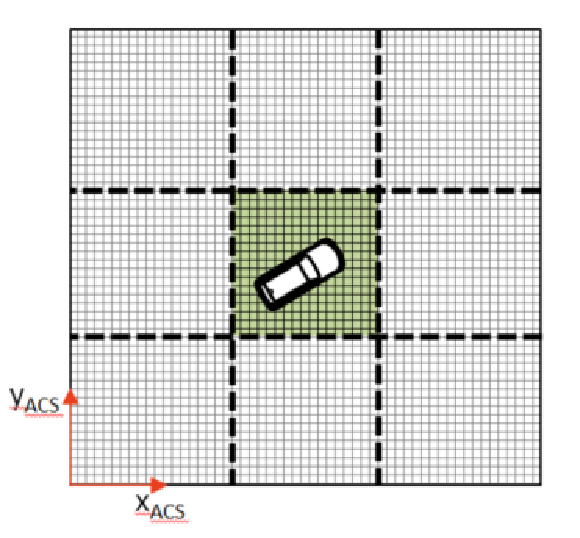
\includegraphics[width=0.5\textwidth]{pics/Diskretisierung der Umgebung.pdf}
	\caption{Anordnung der Position des Autos auf der Karte~\citep{Hegerhorst.2018}}
	\label{fig:Diskretisierung der Umgebung}
\end{figure}
\subsubsection{Zusammenhang zwischen Koordinatensystemen}
Zwischen den oben erl�uterten Koordinatensystemen besteht ein Zusammenhang und die Umrechnung zwischen GCS, ACS und VCS gewinnt bei Implementierung des Umfeldmodells gro�e Bedeutung. Wenn die x-Koordinate des Ankerpunkts anchor\_x und die x-Koordinate des Fahrzeugs pos\_x im GCS bekannt sind, wie in Abbildung~\ref{fig:Koordinaten3} gezeigt, kann die x-Koordinate des Fahrzeugs im ACS durch die Formel offset\_x=pox\_x-anchor\_x erhalten werden. Dabei ist die Umrechnung auf der y-Achse ist analog zur x-Achse. \\Dar�ber hinaus gibt es zwei Punkte, die besondere Aufmerksamkeit erfordern. Das erste ist die Aktualisierung bzw. Initialisierung von ACS. Im Modell wird auch die Zeit diskretisiert, um sich an Computerberechnungen anzupassen. Zu jedem einzelnen Zeitpunkt wird das ACS getestet, ob es aktualisiert werden muss und wie es sich bewegt. Dieser Prozess kann durch das in Abbildung~\ref{fig:ACS_Update} gezeigte Programmablaufdiagramm dargestellt werden. Dabei repr�sentieren X\_1 und X\_2 jeweils die linke und rechte Grenze der X-Achse des gr�n befahrbaren Bereichs in Abbildung~\ref{fig:Diskretisierung der Umgebung}. Y\_1 und Y\_2 repr�sentieren jeweils die unteren und oberen Grenzen des Bereichs. Au�erdem geben dx und dy als positive Werte die Entfernung an, um die der Ursprung des ACS verschoben werden muss. Diese Werte sind so parametriert, dass sie je nach Anwendungsszenario jederzeit ge�ndert werden k�nnen. Dabei beschreiben pox\_x, pox\_y und offset\_x, offset\_y die Position des Fahrzeugs im Weltkoordinatensystem und im Ankerkoordinatensystem. Der Kern des Algorithmus besteht darin, zu �berpr�fen, ob die Position des Fahrzeugs eine bestimmte Grenze �berschritten hat, und sich entsprechend zu bewegen. Wenn beispielsweise offset\_x $>$ X\_2 gilt ist, bedeutet dies, dass die Position des Fahrzeugs die Grenze des befahrbaren Bereichs ber�hrt oder �berschritten hat. In diesem Fall bewegt sich der Anker nach rechts, indem der Wert der x-Koordinate erh�ht wird, sodass das Fahrzeug immer in der Mitte der Rasterkarte bleibt. Dieser ganze Prozess wird als Funktionsmodul mit der Bezeichnung Update ACS betrachtet und zum Entwerfen der Initialisierung von ACS verwendet, wie in Abbildung~\ref{fig:InitializationOfACS} dargestellt. Die Initialisierung des ACS erfolgt gleichzeitig mit der Initialisierung des gesamten Umfeldmodells. Wenn g�ltige Fahrzeugpositionsinformationen erhalten werden, werden die Anfangskoordinaten des Fahrzeugs auch der Anfangsposition des Ankers zugewiesen, wodurch die Anzahl der Bewegungen des ACS verringert wird. Anschlie�end wird mit dem Aktualisierungsmodul die Position des Ankers automatisch angepasst, bis sich die Fahrzeugposition innerhalb des eingestellten Fahrbereichs befindet.
\begin{figure}[ht]
	\centering
	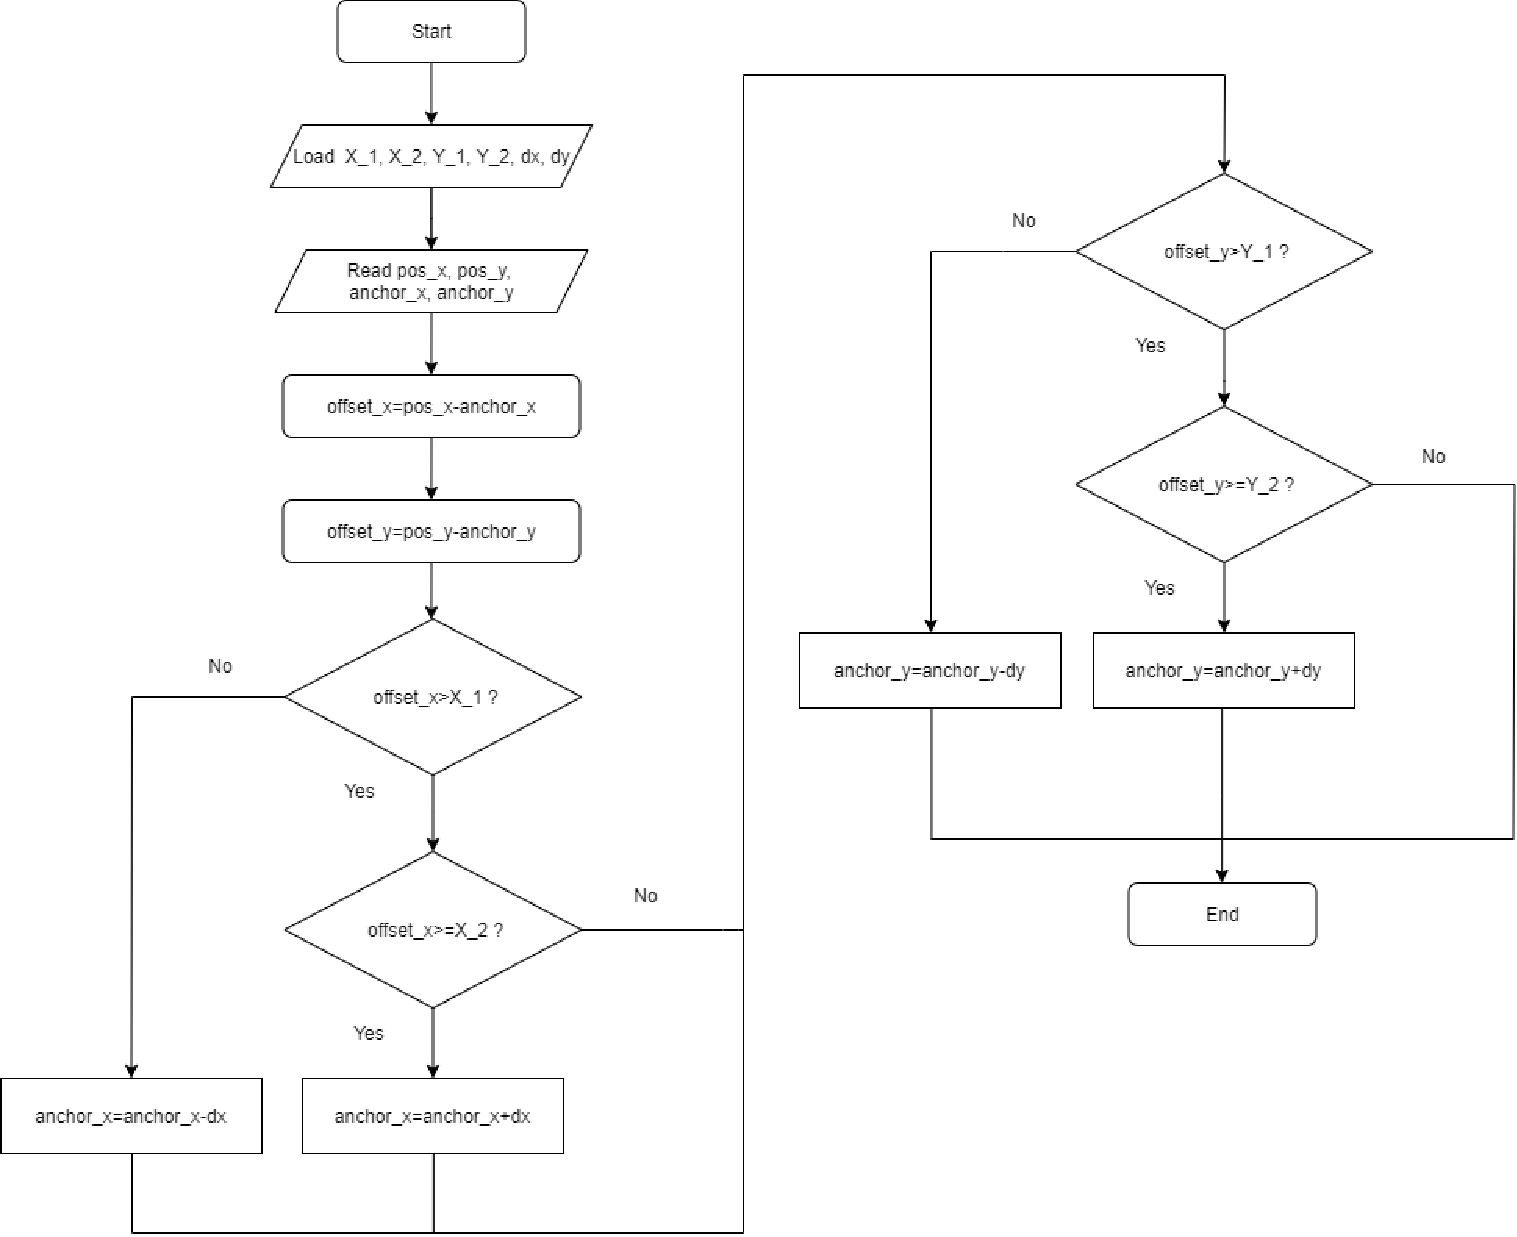
\includegraphics[width=1\textwidth]{pics/ACS_Update.pdf}
	\caption{Programmablaufplan der Aktualisierung von ACS}
	\label{fig:ACS_Update}
\end{figure}
\begin{figure}[ht]
	\centering
	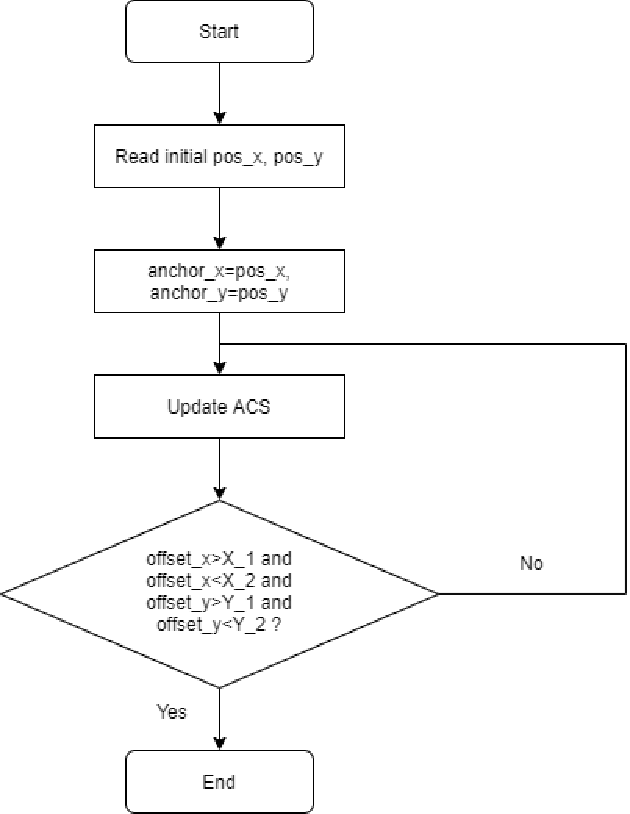
\includegraphics[width=0.7\textwidth]{pics/InitializationOfACS.pdf}
	\caption{Initialisierung von ACS}
	\label{fig:InitializationOfACS}
\end{figure}
\\Der zweite Punkt ist, dass Punktwolkeninformationen und die Visualisierung der Fahrzeugkarosseriestruktur von Koordinaten unter VCS in Koordinaten unter ACS umrechnet werden m�ssen, da der Ausgangspunkt der Diskretisierung Anker ist. Dieser Punkt wird im n�chsten Abschnitt zur Verarbeitung von Sensorinformationen ausf�hrlich erl�utert. 
\subsection{Verarbeitung von Sensordaten}
\label{Verarbeitung von Sensordaten}
F�r das Umfeldmodells in dieser Arbeit sind die beiden wichtigsten Sensorinformationen GPS-Informationen von dGPS-Moduls und Hindernisinformationen von Laserscannern. Unter Verwendung des vorhandenen Frameworks und Algorithmus in IfF werden GPS-Informationen in Form von UTM-Koordinaten angegeben. Wie in Kapitel~\label{Kapitel:Theoretische Grundlagen} erw�hnt, sind im Rahmen dieser Arbeit die beiden Themen Eigenlokalisierung und Umfeldmodellierung entkoppelt, und der Schwerpunkt liegt auf der Umfeldmodellierung. Daher wird hier in Hinsicht auf die Erfassung und Verarbeitung der Daten Laserscannern vertieft eingegangen.
\subsubsection{GPS-Information}
\label{Abschnitt:GPS-Information}
Die wesentliche Information, die GPS liefert, ist die Pose des Fahrzeugs, die die Positionsinformation $pos\_x$ mit $pos\_y$ und Orientierungsinformation $pos\_psi$ enth�lt. Hierbei ist aber zu beachten, dass das ausgew�hlte UTM-Koordinatensystem ein nordweisendes, rechtsdrehendes Koordinatensystem ist~\citep{Hegerhorst.2018}. Daher ist es bei der tats�chlichen Verarbeitung erforderlich, den Richtungswinkel in dem in Abschnitt~\ref{Abschnitt:GCS} erw�hnten linksdrehendes Koordinatensystem GCS durch Berechnung mittels Formel~\ref{Gleichung:Richtungswinkel umrechnen} zu berechnen. Dabei bezeichnet $car\_get\_psi$ die urspr�ngliche Datengr��e des Fahrzeugrichtungswinkels. Diese Umrechnungsbeziehung kann auch durch Abbildung dargestellt werden. Diese Umrechnungsbeziehung kann durch Abbildung~\ref{fig:Richtungswinkel umrechnen} visuell dargestellt werden.
\begin{equation}\label{Gleichung:Richtungswinkel umrechnen}
	pos\_psy=-car\_get\_psi+90^\circ
\end{equation}
\begin{figure}[htbp]
	\centering
	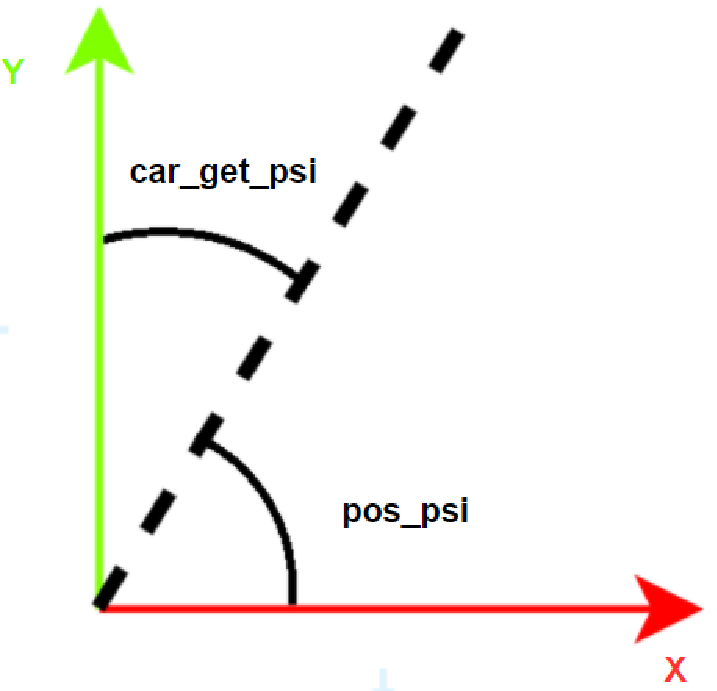
\includegraphics[width=0.4\textwidth]{pics/RichtungswinkelUmrechnen.pdf}
	\caption{Umrechnung des Orientierungswinkels in GCS}
	\label{fig:Richtungswinkel umrechnen}
\end{figure}
\subsubsection{Laserscanner-Information}
\label{Laserscanner-Information}
Die Daten von Ibeo-Laserscanner haben zwei Ausgabeformate. Eines sind Rohdaten, die auf einer Punktwolke basieren, und das andere sind Objektinformationen nach der Verarbeitung von Rohdaten. Die geometrische Form des Objekts ist ein Rechteck. Das vorhandene Framework in IfF verwendet haupts�chlich Objektinformation, um ein Umfeldmodell bzw. eine Rasterkarte zu erstellen. In~\citep{Hegerhorst.2018} werden die Positions- und Gr��eninformationen von Objekten verwendet, gefolgt von Kartierung statischer Hindernisse. Wie in Abbildung~\ref{fig:KartierungMitObjekt} gezeigt, besteht der Kernschritt des Algorithmus darin, die Pose des Objekts in der Rasterkarte zu bestimmen, es als Punktwolkeninformation zu diskretisieren bzw. umrechnen und schlie�lich die belegten Zellen zu markieren. 
\begin{figure}[ht]
	\centering
	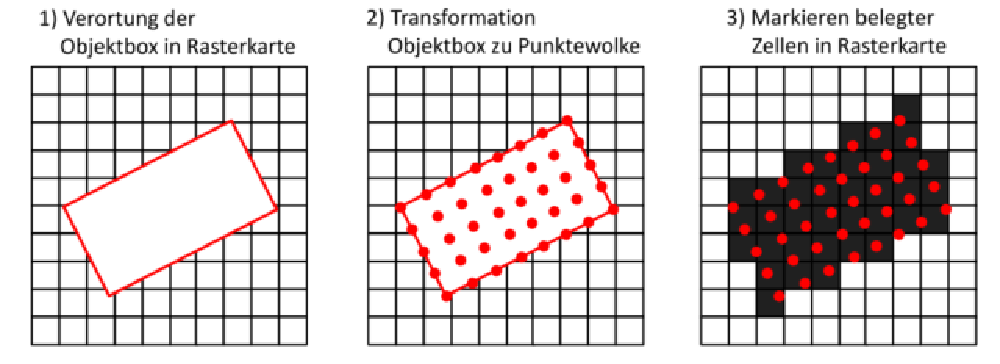
\includegraphics[width=0.7\textwidth]{pics/KartierungMitObjekt.pdf}
	\caption{Kartierungsalgorithmus mit Objektinformation von Laserscanner~\citep{Hegerhorst.2018}}
	\label{fig:KartierungMitObjekt}
\end{figure}
Die Verwendung dieses Ansatzes weist jedoch mehrere Nachteile auf. Wie in Kapitel~\ref{Kapitel:Theoretische Grundlagen} erl�utert, besteht einer der Vorteile der Verwendung des gitterbasierten Modells darin, dass es Hindernisse beliebiger Form ausdr�cken kann. Bei Verwendung der Objektinformationen werden Hindernisse in diesem Fall jedoch immer durch Rechtecke dargestellt, wodurch dieser Vorteil zunichte gemacht wird. Zweitens werden in tats�chlichen Anwendungen z.B. mehrere diskrete Punkte als kontinuierliches Hindernis falsch eingesch�tzt. Au�erdem werden die Scanpunkte langer gerader Objekte hart durch einen Box dargestellt und daher in kleinere Boxen aufgeteilt oder gar nicht nicht ausgegeben\citep{Hegerhorst.2018}.  Dies f�hrt zu Ungenauigkeiten und geringer Qualit�t des Modells. Schlie�lich erfordert die Verwendung von Objektinformationen einen weiteren Schritt zur Umwandlung in eine Punktwolke, was den Rechenaufwand erh�ht. Es ist direkter und nat�rlicher, die Punktwolkeninformationen des Laserscanners direkt zu verwenden.
\\Als n�chstes wird die Verarbeitung von Punktwolkeninformationen mittels des in Abbildung~\ref{fig:PAP_PCL} gezeigte Flussdiagramm ausf�hrlich erl�utert. Der Ibeo-Laserscanner liefert �ber den ROS-Treiber verschiedene Dateninformationen und publiziert diese zu den entsprechenden Topics. Das wichtigste ist, dass Topic $as\_tx/point\_cloud$ Information liefert, deren Messagetyp $sensor\_msgs/PointCloud2$ ist. Es ist anzumerken, dass diese Daten tats�chlich vom Datentyp \textless$pcl::PointXYZL$\textgreater~der PCL-Standardbibliothek gekapselt und geliefert werden. Daher wird in der tats�chlichen Codeimplementierung Zeiger (engl. pointer) verwendet, um die 4 Beschreibungsinformationen der Punktwolke in \textless$pcl : : PointXYZL$\textgreater~zu lesen. Sie handelt sich um X-, Y- und Z-Koordinaten des Fahrzeugkoordinatensystems und der Schicht (engl. layer), in der sich die Punktwolke befindet.
\begin{figure}[ht]
	\centering
	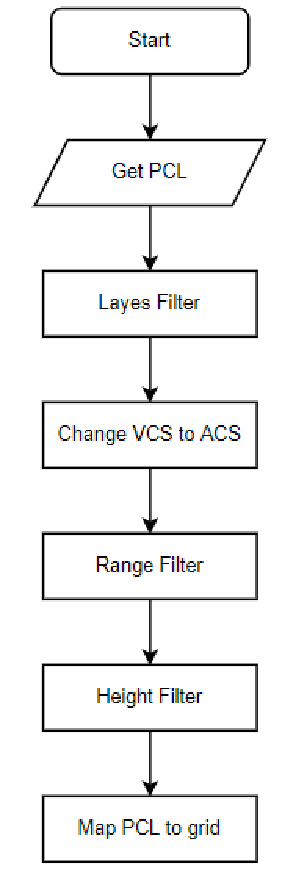
\includegraphics[width=0.28\textwidth]{pics/PAP_PCL.pdf}
	\caption{Programmablaufplan der Laserscannerdaten}
	\label{fig:PAP_PCL}
\end{figure}
\\Im Versuchsfahrzeug Passat (siehe Abbildung~\ref{fig:AnordnungDerLaserscanner}) sind Sensor 2 und Sensor 5 am Fahrzeug mit Ibeo-LUX-8L ausgestattet. Die restlichen Laserscanner sind Ibeo-LUX-4L. Ibeo-LUX-8L wird tats�chlich durch die Drehung des Objektivs konstruiert, um den vertikalen Erfassungsbereich zu verdoppeln. Wenn es in Kombination mit Ibeo-LUX-4L verwendet wird, ist der Erfassungsbereich zu zwei benachbarten Zeitpunkten bei derselben Frequenz inkonsistent. Beispielsweise ist die bei Zeitpunkt $t_1$ erfasste Punktwolke nur in den Schichten 0 bis 3 verteilt, w�hrend die bei $t_2$ erfasste Punktwolke sich einschlie�lich in den Schichten 4 bis 7 befinden. Diese Inkonsistenz kann durch Bin�r-Bayes-Filter die Korrektheit und Stabilit�t des Modells beeintr�chtigen. Aus diesem Grund wird im Funktionsblock $Layes Filter$ das Datenframe, das 4 bis 7 Schichten von Punktwolkeninformationen enth�lt, verworfen. Diese Methode ist direkt und einfach und verbessert nachweislich die Stabilit�t des Modells.
\\Im Funktionsblock $Change VCS to ACS$ wird die im Fahrzeugkoordinatensystem vorliegende Position jedes Punkt von Punktwolke in Ankerkoordinatensystem umgerechnet. Um die Umrechnung durchzuf�hren, ist ein Hilfskoordinatensystem (HCS), wie in Abbildung~\ref{fig:VCS2ACS} gezeigt, erstellt.
\begin{figure}[ht]
	\centering
	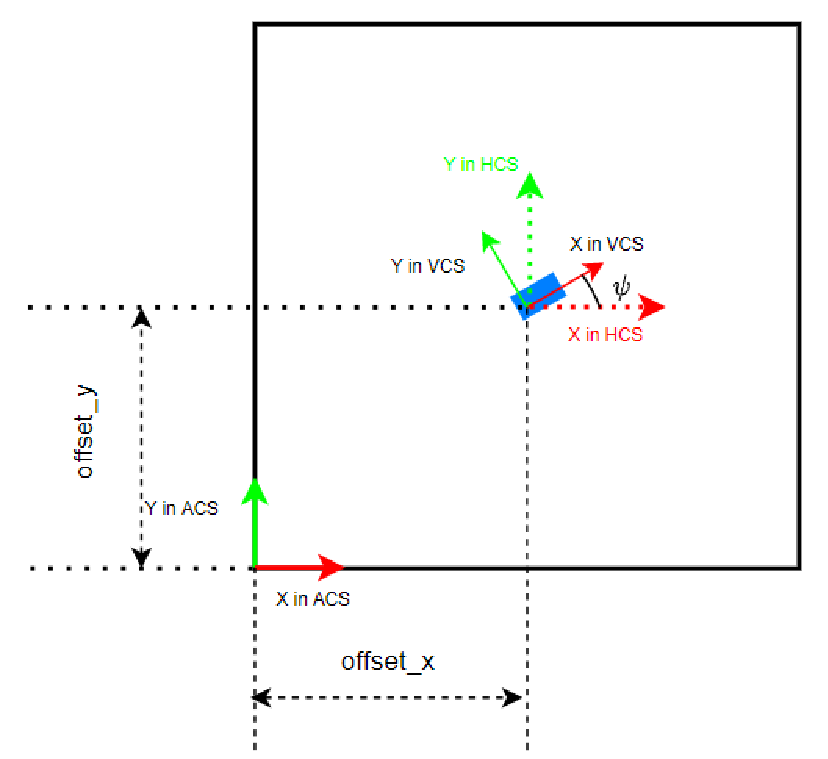
\includegraphics[width=0.7\textwidth]{pics/VCS2ACS.pdf}
	\caption{Darstellung eines Hilfskoordinatensystem}
	\label{fig:VCS2ACS}
\end{figure}
Dann l�sst sich die Koordinatenumwandlung in 2 Schritte zerlegen. Der erste Schritt besteht darin, das Referenzkoordinatensystem jedes Punktes von ACS in HCS umzuwandeln. Die mathematische Beschreibung dieses Schritts ist in Gleichung~\ref{Gleichung:RotaionTransform} gezeigt.
\begin{equation}\label{Gleichung:RotaionTransform}
	{}^{H}\textbf{P}_{}={}^{H}\textbf{R}_{V}~{}^{V}\textbf{P}_{}
\end{equation} 
Dabei bezeichnet ${}^{V}\textbf{P}_{}$ und ${}^{H}\textbf{P}_{}$ den Koordinatenvektor eines bestimmten Punktes in VCS bzw. HCS. Die lassen sich mit~Gleichung~\ref{Gleichung:V_P} und~\ref{Gleichung:H_P} beschreiben. 
\begin{equation}
	\label{Gleichung:V_P}
	{}^{V}\textbf{P}_{} = 
	\begin{pmatrix}
		{}^{V}{x}_{}\\
		{}^{V}{y}_{}\\
	\end{pmatrix}
\end{equation}
\begin{equation}
	\label{Gleichung:H_P}
	{}^{H}\textbf{P}_{} = 
	\begin{pmatrix}
		{}^{H}{x}_{}\\
		{}^{H}{y}_{}\\
	\end{pmatrix}
\end{equation}
${}^{H}\textbf{R}_{V}$ ist als Drehmatrix oder Rotationsmatrix genannt und ihre konkrete Beschreibung befindet sich in Gleichung~\ref{Gleichung:RotaionMatrix}. Darunter wird der Wert von $pos\_psi$ direkt f�r $\psi$ verwendet, da GCS und ACS immer in die gleiche Richtung zeigen. 
\begin{equation}
	\label{Gleichung:RotaionMatrix}
	{}^{H}\textbf{R}_{V} = 
	\begin{pmatrix}
		cos(\psi) & -sin(\psi)\\
		sin(\psi) & cos(\psi)\\
	\end{pmatrix}
\end{equation}
Der zweite Schritt ist die Umwandlung von HCS in ACS, die durch einfache Vektoraddition erhalten wird. Die mathematische Formel befindet sich in~\ref{Gleichung:HCS2ACS}. Analog bezeichnet ${}^{A}\textbf{P}_{}$ den Positionsvektor in ACS. Offset-Vektor D stellt die Abweichung von ACS und HCS dar, sodass kein bestimmtes Koordinatensystem angegeben werden muss.
\begin{equation}\label{Gleichung:HCS2ACS}
	{}^{A}\textbf{P}_{}={}^{H}\textbf{P}_{}+\textbf{D}
\end{equation}
mit
\begin{equation*}
	\textbf{D} = 
	\begin{pmatrix}
		offset\_x\\
		offset\_y\\
	\end{pmatrix}
\end{equation*} und \begin{equation*}
	{}^{A}\textbf{P}_{} = 
	\begin{pmatrix}
		{}^{A}{x}_{}\\
		{}^{A}{y}_{}\\
	\end{pmatrix}
\end{equation*}
Zusammenfassend kann die x-Koordinate und die y-Koordinate des Punktes im ACS unter Verwendung der Gleichungen~\ref{Gleichung:XinACS} bzw. \ref{Gleichung:YinACS} berechnet werden.
\begin{equation}\label{Gleichung:XinACS}
	{}^{A}{x}_{}=cos(\psi)\times{}^{V}{x}_{}-sin(\psi)\times{}^{V}{y}_{}+offset\_x
\end{equation}
\begin{equation}\label{Gleichung:YinACS}
	{}^{A}{y}_{}=sin(\psi)\times{}^{V}{x}_{}+cos(\psi)\times{}^{V}{y}_{}+offset\_y
\end{equation}
Funktionsblock $Range~Filter$ in Abbildung~\ref{fig:PAP_PCL} handelt sich um, dass alle Punkte von Punktwolken au�er Erfassungsbereich bzw. Umfeldmodelldimension ausgefiltert werden. In �bereinstimmung mit dem IfF-Framework verf�gt die Umfeldmodell bzw. Rasterkarte �ber 400$\times$400 Gitterzellen. Jede Gitterzelle ist 0,25 m$\times$0,25 m gro�, daher wird auch die Aufl�sung der Rasterkarte als 0,25 m bezeichnet. In diesem Fall werden alle erfasste Punkte herausgefiltert, deren x- oder y-Koordinate 100 m im ACS-Koordinatensystem �berschreitet. Nat�rlich werden auch die Anzahl der Gitterzellen und die Aufl�sung der Karte so parametrisiert, dass sie sich entsprechend den tats�chlichen Anwendungsanforderungen �ndern k�nnen. Durch das Anordnen des Funktionsblocks $Range~Filter$ vor der Kartierung des Hindernis k�nnen unn�tige Daten im Voraus verworfen und nutzlose Berechnungen vermieden werden.
\\Obwohl das Umfeldmodell in dieser Arbeit ein zweidimensionales Occupancy-Grid ist, enth�lt die vom Ibeo-Laserscanner erhaltene Punktwolke tats�chlich dreidimensionale Informationen. Daher hat es die H�heninformationen des Punktes $z$. Im Funktionsblock $Height~Fitler$ ist die zu erkennende H�he begrenzt und zu hohe oder zu niedrige Daten werden herausgefiltert. Dies kann erstens die abnormalen Punktwolkeninformationen beseitigen und zweitens die Anzahl von Punktwolken unterschiedlicher H�he an derselben Stelle verringern, wodurch die Berechnungslast verringert wird. Der Grund liegt daran, dass der Beitrag von Punktwolken am selben Ort und in unterschiedlichen H�hen zum 2D-Umfeldmodell gleich und redundant ist. 
\\Im Funktionsblock $Map~PCL~to~grid$ wird die Punktwolke in den diskretisierten Gitterzellen weiter abgebildet. In der Implementierung wird ein zweistelliges 400$\times$400-Array erstellt, und jedes ihrer Gitterzelle hat einen Index in x- und y-Richtung. Jede Punktwolkeninformation wird durch Gleichung~\ref{Gleichung:Index_X} und~\ref{Gleichung:Index_Y} in einen Gitterindex umgewandelt, wobei dieses Gitter als belegt markiert wird. Im Rahme dieser Arbeit wird das Ergebnis in einem zweidimensionalen Array namens $pcl_grid$ gespeichert.
\begin{equation}
	\label{Gleichung:Index_X}
	Index\_x\approx {}^{A}{x}_{}/GS
\end{equation}
\begin{equation}
	\label{Gleichung:Index_Y}
	Index\_y\approx {}^{A}{y}_{}/GS
\end{equation}
In der Gleichungen ist GS (Grid Spacing) die Aufl�sung der Rasterkarte. Die Rundung in den Gleichungen bedeutet, dass die berechneten Daten abgerundet werden, bevor sie als Indexparameter verwendet werden k�nnen. Dar�ber hinaus hat das wiederholte Markieren eines Quadrats keine Auswirkung.
\subsubsection{Synchronization der Sensordaten}
\label{Synchronization der Sensordaten}
Unterschiedliche Sensordaten stammen aus in ROS unterschiedlichen Kan�len bzw. Themen. Die Sicherstellung der Zeitsynchronisation dieser Daten ist f�r die Echtzeitgenauigkeit des Modells sehr wichtig. Beispielsweise bleiben die Sensorinformationen von Lidar hinter den Informationen von GPS zur�ck, was dazu f�hrt, dass die Hindernisinformationen um das Fahrzeug nicht rechtzeitig aktualisiert werden und das Modell daher ungenau ist. In ROS wird jede Informationsfreigabe von einem Zeitstempel (engl. timestamp) begleitet. Der $ApproximateTime~Policy$ Algorithmus in der Bibliothek (engl. library) von $message\_filters$ wird verwendet, um sicherzustellen, dass die Zeitstempel von Sensorinformationen aus verschiedenen Datenquellen sehr nahe oder fast gleich sind, z. B. 10 Femtosekunde (fs). Informationen, die diesen Schwellenwert �berschreiten, werden als ung�ltig betrachtet und verworfen. Dieses Verfahren stellt nicht nur die Synchronisation von Informationen sicher, sondern kann auch die aktuellen Rahmendaten filtern, wenn eine bestimmte Datenquelle abnormal ist, wodurch die Genauigkeit der Daten sichergestellt wird.
\subsection{Implementierung von Occupancy Grid}
Nach der Einf�hrung von Koordinatensystemen und der Beschreibung der Sensordatenverarbeitung wird in diesem Abschnitt der Kern des Modells, die Implementierung von Occupancy Grid, erl�utert. Sie umfasst die Implementierung von 2 Ebenen, wie in Abbildung~\ref{fig:EbeneVonOccupancyGrid} dargestellt.
\subsubsection{Raumdiskretisierung}
Auf dieser Ebene wird die Umgebung des Fahrzeugs diskretisiert und als 2D-Rasterkarte beschrieben. Im ersten Schritt werden die L�nge und Breite des Erfassungsbereichs bestimmt, und im zweiten Schritt wird die Aufl�sung der Rasterkarte bzw. die Gr��e jeder Gitterzelle festgestellt. Daraus ergibt sich die Anzahl der Zelle im gesamten Modell. Diese Werte sind parametrisiert und bieten eine Schnittstelle f�r nachfolgende �nderungen gem�� verschiedenen Anwendungsszenarien. Im Rahme dieser Arbeit wird das Umfeldmodell zur Anpassung an das IfF-Framework als 400$\times$400-Gitter beschrieben, wobei jede Gitterzelle 0,1$\times$0,1 Quadrat ist. Dies bedeutet, dass der Fahrzeugerkennungsbereich eine Fl�che von 40 x 40 m betr�gt. Es ist sehr nat�rlich, ein zweidimensionales Array in C++ zu verwenden, um dieses Raster zu beschreiben, das eine bestimmte Zelle im Raum direkt indizieren und den entsprechenden zus�tzlichen Wert lesen kann. Hierbei werden zwei zweidimensionale Arrays erstellt, n�mlich $current\_grid$ und Verlauf $history\_grid$. Ersteres wird verwendet, um die vom inversen Sensormodell erhaltenen Wahrscheinlichkeitsverteilungen zu speichern, n�mlich $p(m_i|z_t)$ in Gleichung~\ref{Gleichung:Ableitung_06}. Letzteres wird verwendet, um die historisch akkumulierten A-posteriori-Wahrscheinlichkeit nach der Bayes-Filterung zu speichern, die in Gleichung~~\ref{Gleichung:Ableitung_06} als $p(m_i|z_{1:t-1})$ bezeichnet wird. Im aktuellen Frame wird der berechnete $bel_t(m_i)$ als Daten im $hitory\_grid$ des n�chsten Frames verwendet.
\subsubsection{Probabilistischer Ansatz}
\label{Probabilistischer Ansatz}
Der erste Schritt in dieser Ebene ist die Zuweisung von $current\_grid$, bei der die aktuelle Belegungswahrscheinlichkeit jeder Zelle gem�� den Sensorinformationen ermittelt wird. Dies bedeutet, dass die Implementierung des in Abschnitt~\ref{Abschnitt:Das zu verwendende Sesormodell} genannten inversen Sensormodells. Wie in Abschnitt~\ref{Abschnitt:Das zu verwendende Sesormodell} erw�hnt, wird das in dieser Arbeit verwendete Sensormodell durch zwei eindimensionale abschnittsweise definierte Funktionen beschrieben und f�r einen einzelnen Strahl verwendet. Die verschiedenen Lichtstrahlen, die von jedem Sensor emittiert werden, werden von demselben Modell beschrieben. 
\\Der Implementierungsalgorithmus kann durch das in Abbildung~\ref{fig:ImplementierungDesSensormodells} gezeigte Flussdiagramm dargestellt werden.
\begin{figure}[htbp]
	\centering
	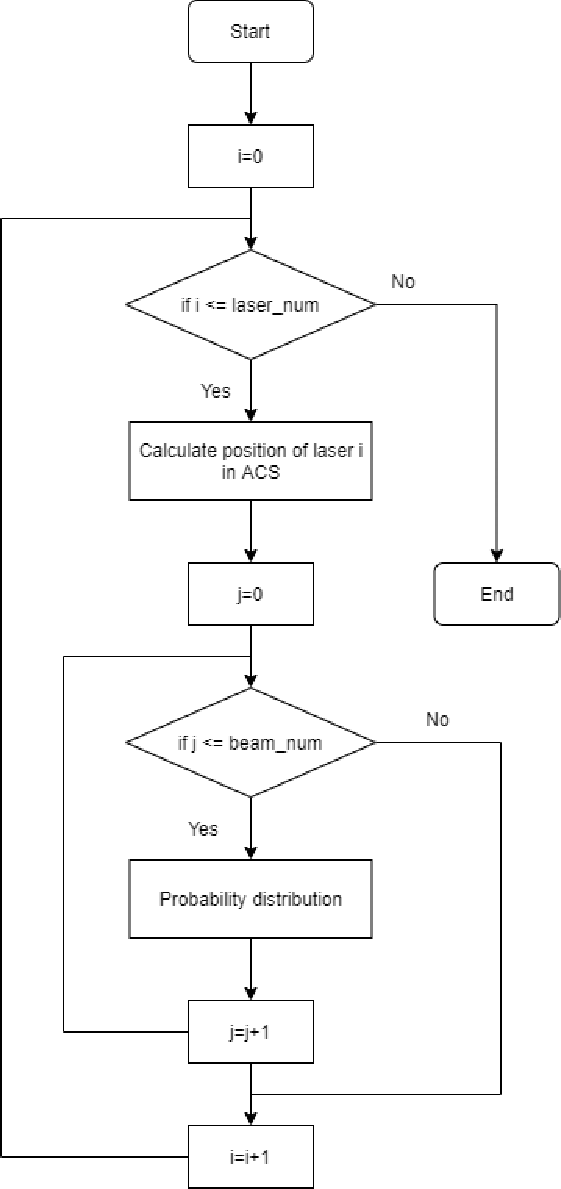
\includegraphics[width=0.7\textwidth]{pics/ImplementierungDesSensormodells.pdf}
	\caption{Implementierung des inversen Sensormodells}
	\label{fig:ImplementierungDesSensormodells}
\end{figure}
Hier werden zwei Schleifen verwendet. Die �u�ere Schleife repr�sentiert die Behandlung verschiedener Laserscanner am Fahrzeug. Die Zahl $laser\_num$ repr�sentiert die Anzahl der Sensoren im Fahrzeug. Die innere Schleife bezeichnet die Verarbeitung verschiedener emittierter Lichtstrahlen von einem einzelnen Sensor. Dabei ist $beam\_num$ die Anzahl dieser Strahlen ist, die durch Dividieren des horizontalen �ffnungswinkels des Laserscanners durch die horizontale Winkelaufl�sung erreicht wird.
\\Der Funktionsblock $Calculate~position~of~laser~i~in~ACS$ dient zur Bestimmung der Ortskoordinaten des Laserscanners, dessen ID $i$ ist. Die Positionsinformationen des Sensors als Eingabeparameter des Umfeldmodell werden mit dem Fahrzeugkoordinatensystem als Referenzsystem angegeben. Die Erstellung des Umfeldmodell basiert auf dem Ankerkoordinatensystem, daher m�ssen die Koordinaten der Sensorposition auch in ACS bestimmt werden. Das Wesentliche dieses Problems ist immer noch das in Abschnitt~\ref{Laserscanner-Information} erw�hnte Problem der Konvertierung von VCS in ACS, daher wird die Er�rterung hierbei nicht wiederholt.
\\Den Zellen in Strahlrichtung werden je nach Abstand zum Laserscanner unterschiedliche Wahrscheinlichkeitswerte im Funktionsblock $Probability~distribution$ zugeordnet. Als eine Linie wird der eindimensionale Strahl vom ber�hmten Bresenham-Algorithmus
realisiert. Wie in Abbildung~\ref{fig:Raycasting} gezeigt, wird beispielsweise der aktuell verarbeitete Lichtstrahl durch eine blaue durchgezogene Linie dargestellt. 
\begin{figure}[htbp]
	\centering
	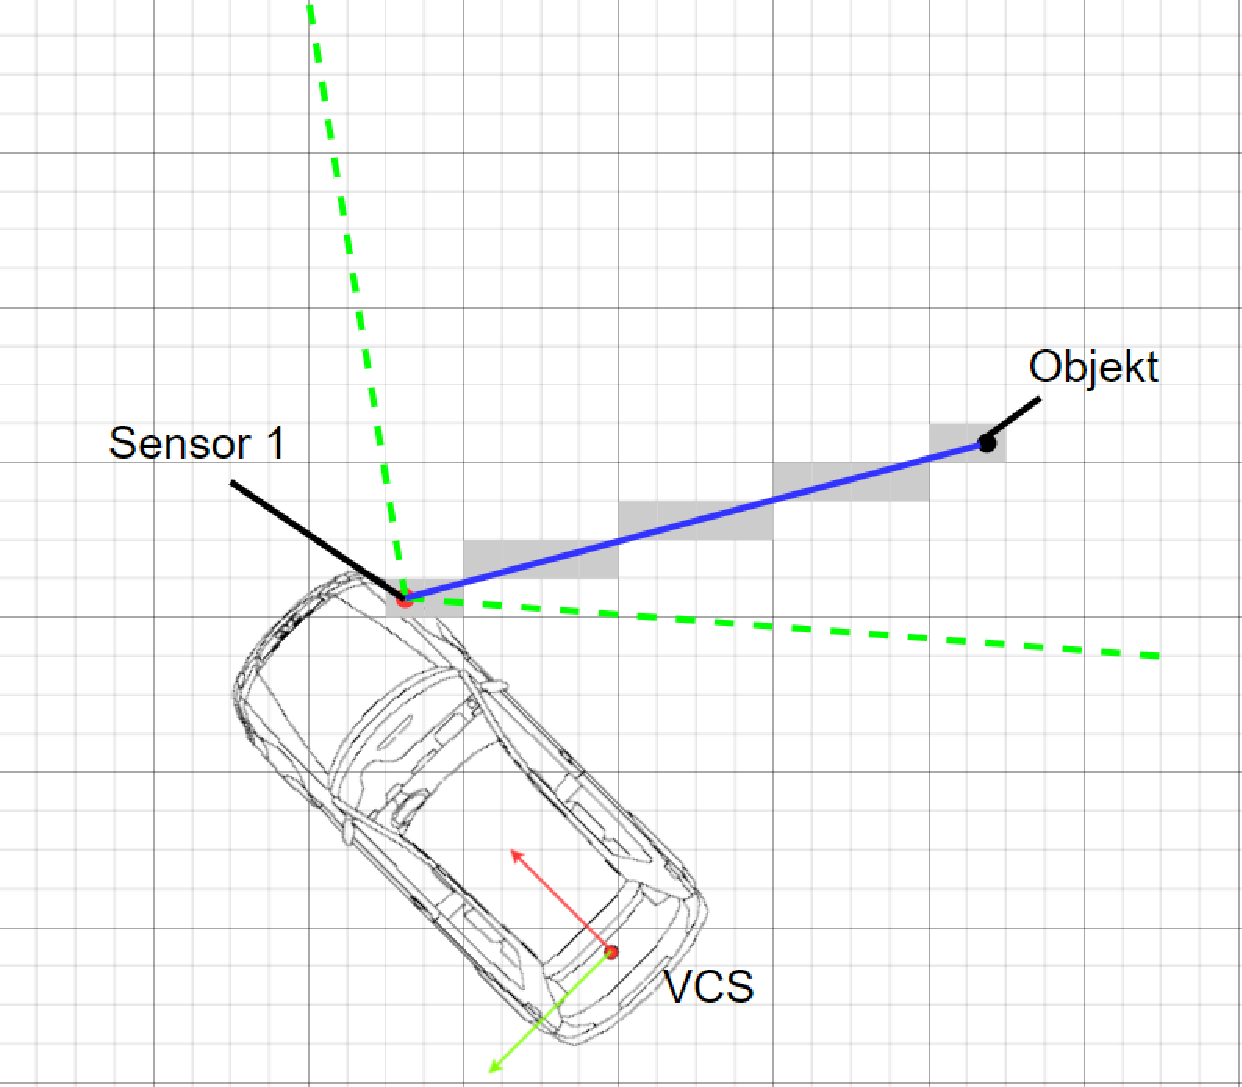
\includegraphics[width=0.7\textwidth]{pics/Raycasting.pdf}
	\caption{Raycasting mit Bresenham-Algorithmus}
	\label{fig:Raycasting}
\end{figure}
Der rote Punkt zeigt die aktuelle Position des zu verarbeitenden Sensors an und dient als Startpunkt des Strahls. Der schwarze Punkt repr�sentiert die Position des Objekts und dient als Ende des Strahls. Unter Anwendung von dem Bresenham-Algorithmus werden die Zellen, denen tats�chlich Wahrscheinlichkeitswerte zugewiesen werden, grau dargestellt. Der gr�n gestrichelte Teil stellt den Bereich dar, den der Sensor scannen kann. Die gr�ne gestrichelte Linie stellt den Bereich dar, den der Sensor scannen kann. In diesem Bereich wird in verschiedene Richtungen durch die oben erw�hnte innere Schleife mit dem Schritt von der Winkelaufl�sung abgetastet. Dies wird auch als Raycasting bezeichnet. In Bezug auf den spezifischen Wahrscheinlichkeitswert haben die Elemente von $current\_grird$, das den Zellen entspricht, die in dem in Abschnitt~\ref{Laserscanner-Information} genannten $pcl\_grid$ als belegt markiert sind, den Wert von $p\_fill$. Wird beispielsweise die Position $(3, 4)$ von $pcl\_grid$ als belegt markiert, wird der Wert $p\_fill$ dem Element $(3, 4)$ des Arrays von $current\_grid$ zugewiesen. Den Zellen innerhalb des minimal erkennbaren Abstands wird $p\_clear$ zugewiesen. Die Wahrscheinlichkeitsverteilung der in der Mitte bestehenden Zellen  werden durch eine lineare Funktion dargestellt, und ihre Steigung wird durch eine Variable $p\_slope$ dargestellt. Der Sensor erkennt, dass sich an einem bestimmten Ort ein Hindernis befindet, oder der Sensor liefert die Information, dass sich kein Hindernis befindet. Diese beiden Situationen weisen eine unterschiedliche Genauigkeit auf. Die Variable $p\_clear$ und $p\_fill$ sind jeweils ein Indikator f�r die Genauigkeit dieser beiden Situationen. Die Variable $p\_slope$ verk�rpert, wie weit die Sensordaten von der Entfernung zwischen dem Objekt und dem Laserscanner beeinflusst werden. Die oben genannten drei Variablen m�ssen entsprechend den tats�chlichen Anwendungen und Szenarien sowie den Eigenschaften und der Qualit�t der verwendeten Sensoren angepasst werden. Anderen Zellen in der Karte wird ein Wahrscheinlichkeitswert von $50\%$ als Bereiche zugewiesen, die vom Sensor nicht erkannt werden k�nnen.
\\Nach Abschluss der Zuweisung aller Elemente im $current\_grid$ besteht der n�chste Schritt in dieser Ebene darin, den bin�ren Bayes-Filter zu verwenden, um die Belegungswahrscheinlichkeit jeder Zelle vom aktuellen Zeitstempel zu aktualisieren. Hierbei wird das Array $history\_grid$ verwendet, um die Belegungswahrscheinlichkeiten des letzten Zeitstempels zu speichern. Der Berechnungsprozess wird durch Gleichung~\ref{Gleichung:Ableitung_06} realisiert. F�r jede Zelle repr�sentiert der Term $p(m_i|z_t)$ den in $current\_grid$ gespeicherten Wert und der Term $p(m_i|z_{1:t-1})$ den in $history\_grid$ gespeicherten Wert. Der berechnete Term $bel_t(m_i)$ wird als der Wert in $history\_grid$ des n�chsten Zeitstempels verwendet. Es ist erw�hnenswert, dass jedem Element von $history\_grid$ im Ausgangszustand $50\%$ zugewiesen werden, da keine Vorkenntnisse �ber die Umgebung vorliegen. Bevor der bin�re Bayes-Filter angewendet wird, muss au�erdem �berpr�ft werden, ob die Karte verschoben wurde. Wenn der Ort der Karte bzw. der Ankerpunkt nicht mit dem Ort des vorherigen Zeitstempels �bereinstimmt, muss das Array $history\_grid$ entsprechend der Bewegungsrichtung und dem Schritt der Bewegung aktualisiert werden. Wie in Abbildung~\ref{fig:MoveOfMap} gezeigt, wird ein 16$\times$16-Raster verwendet, um dieses Problem zu veranschaulichen. 
\begin{figure}[ht]
	\centering
	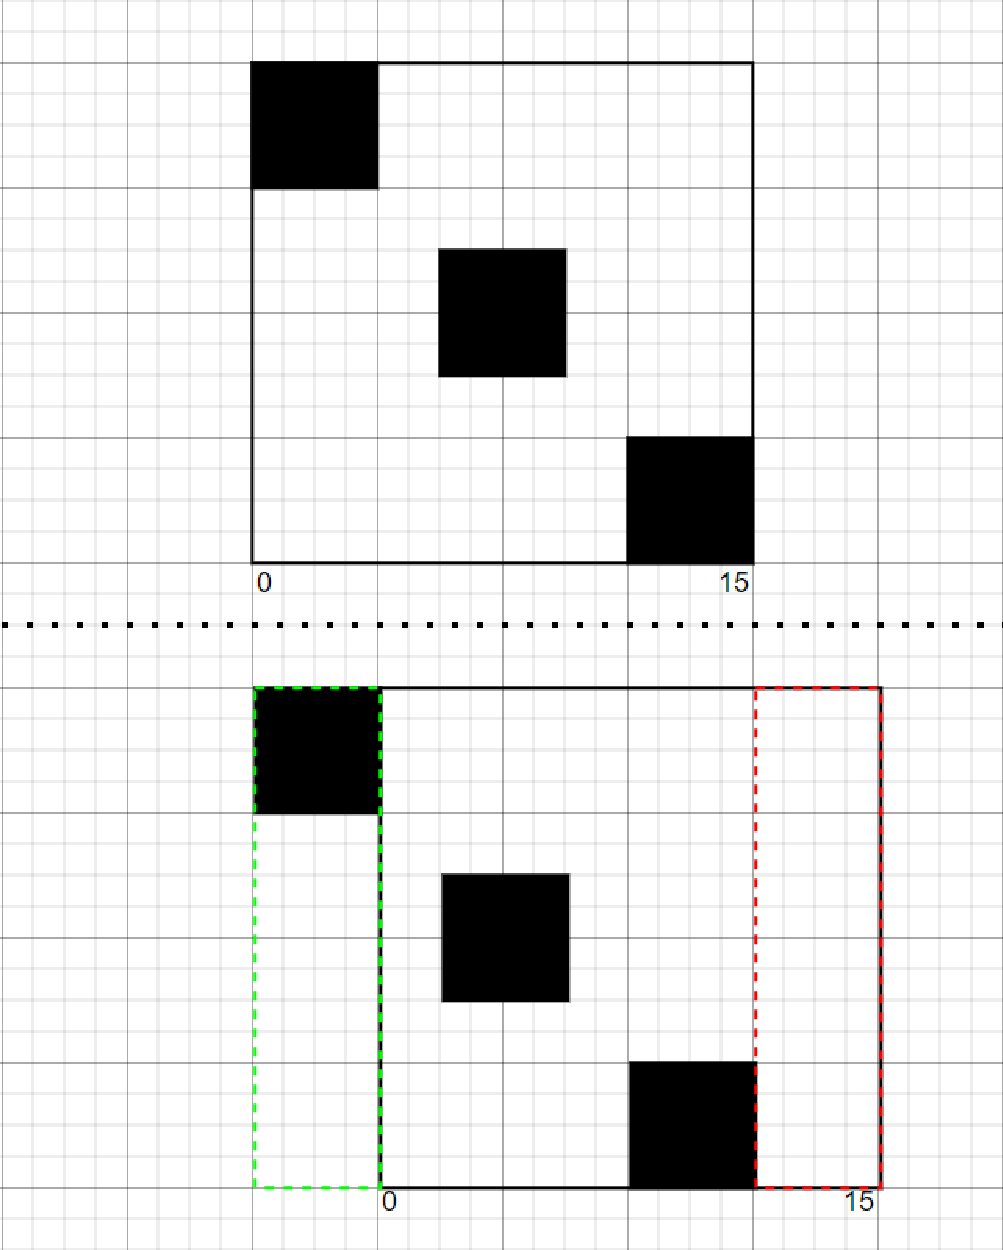
\includegraphics[width=0.7\textwidth]{pics/MoveOfMap.pdf}
	\caption{Aktualisierung vom Array $Hisotry\_grid$ aufgrund der Verschiebung der Karte}
	\label{fig:MoveOfMap}
\end{figure}
Der obere Teil der Abbildung zeigt die Karte mit dem Zeitstempel t und der untere Teil zeigt die verschobene Karte mit dem Zeitstempel t + 1. In der oberen linken Ecke, der unteren rechten Ecke und der Mitte dieser Karte befinden sich Hindernisse, die durch schwarze Quadrate gekennzeichnet sind. Gleichzeitig wird ein 16$\times$16-Array erstellt und Wahrscheinlichkeitswerte zugewiesen. Es wird angenommen, dass zum Zeitpunkt $t+1$ die Karte $4$ Zellen nach rechts verschoben hat. Dann entspricht der Bereich, der durch Elemente dargestellt wird, deren x im neuen $history\_array$ gleich $0$ bis $11$ ist, dem Bereich, der durch Elemente von $4$ bis $15$ im alten $history\_grid$ dargestellt wird. Die gr�n markierten Bereiche werden im Modell nicht mehr ber�cksichtigt. Im rot angezeigten Bereich sind keine Sensordaten zu diesem Zeitpunkt vorhanden sind. Daher sollten die Elemente in diesem Bereich mit einem Wahrscheinlichkeitswert von $50\%$ initialisiert werden. Der eigentliche Prozess muss die vier Bewegungsrichtungen und Bewegungsentfernungen ber�cksichtigen.
\subsection{Zus�tzliche Features}
Nach der Erstellung des Umfeldmodells werden dem System einige zus�tzliche Funktionen f�r die sp�tere Erweiterung und den Informationsaustausch mit anderen Systemen hinzugef�gt.
\subsubsection{Ausgangsinformationsfluss}
Am Ausgang des Systems sind, wie in Abbildung~\ref{fig:OutputFluss} dargestellt, zwei wichtige Ausgabedaten geplant. 
\begin{figure}[htbp]
	\centering
	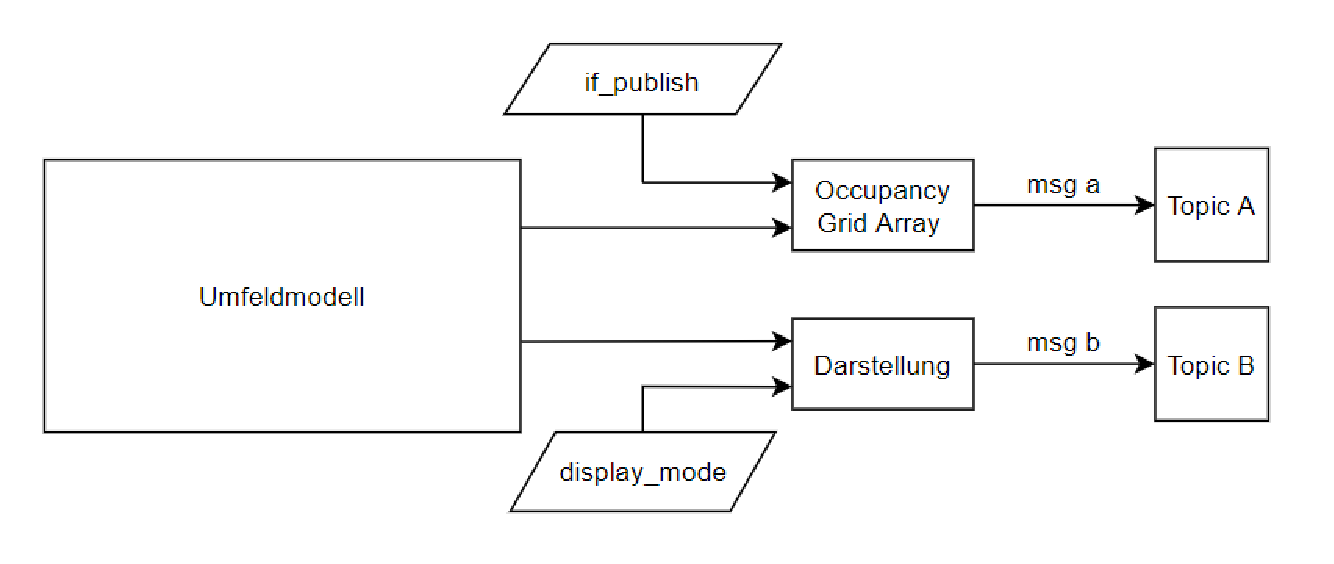
\includegraphics[width=0.7\textwidth]{pics/OutputFluss.pdf}
	\caption{Ausgangsinformationsfluss}
	\label{fig:OutputFluss}
\end{figure}
Die erste besteht darin, das Array auszugeben, das Occupancy Grid im aktuellen Modell darstellt. Jedes Element des Arrays hat seine Belegungswahrscheinlichkeit. Aufgrund der Eigenschaften des ROS-message ist das Ausgabearray ein eindimensionales Array. Daher muss in diesem Schritt das im System vorhandene zweidimensionale Array in ein eindimensionales Array eingekapselt werden. In einem anderen ROS-node, der die Daten empf�ngt, k�nnen das wieder in ein zweidimensionales Array umgerechnet werden. Zu diesem Zweck muss die Gr��e jeder Dimension des Arrays angegeben werden. Da die Wahrscheinlichkeitsgenauigkeit von $1\%$ ausreichend ist, ist die jeder Zelle zugewiesene Wahrscheinlichkeit eine Ganzzahl zwischen 0 und 100. In diesem Fall wird das Array aufgrund Speicherbedarf als Uint8-Datentyp erstellt. Die Variable $if\_publish$ wird verwendet, um zu entscheiden, ob die Ros-message im entsprechenden Ros-topic geliefert werden soll.
\\Die zweite ausgegebene Information wird verwendet, um sie in einer verwandten ROS-topic zur Visualisierung in ROS-Rviz zu liefern. Der Parameter $display\_mode$ legt fest, wie das umfeldmodell visualisiert wird. Wie in Abschnitt~\ref{Visualisierung des Umfeldmodells in ROS} erw�hnt, umfassen die Visualisierungstypen $Gridcell$ und $binarized~Gridcells$.
\subsubsection{Visualisierung des Fahrzeugs}
Die Bestimmung der r�umlichen Position des vom Fahrzeug abgedeckten Bereichs im Modell ist nicht Teil des Umgfeldmodells, aber hilfreich f�r die sp�tere kollisionsfreie Navigation. Gleichzeitig tr�gt die Visualisierung dieses Bereichs zur Vollst�ndigkeit der Umfeldmodellvisualisierung bei. Um den vom Fahrzeug abgedeckten Bereich zu beschreiben, wird gem�� den Daten in Tabelle~\ref{tab:Abmessung von Versuchsfahrzeuge} und der Position des Ursprungs des Fahrzeugkoordinatensystems ein Rechteck erstellt, das den Fahrzeugbereich abdeckt. Dann wird das Rechteck in Punkte diskretisiert, um eine Punktwolke zu bilden. Wie die Position der Punktwolke von VCS in ACS umrechnet und dann kartiert wird, wurde in Abschnitt~\ref{Laserscanner-Information} erl�utert. In �hnlicher Weise kann das Fahrzeug auch durch einige nahe gelegene Zellen dargestellt werden, die mittels einer einzigen ROS-topic in ROS-Rviz visualisiert werden k�nnen. Das tats�chliche Visualisierungsergebnis sind in Abbildung~\ref{fig:Display_Map} als den blauen Bereich dargestellt.
\subsubsection{Visualisierung von Bewegungspfaden}
F�r die Bed�rfnisse der nachfolgenden Navigation wird im Rahmen dieser Arbeit auch die Visualisierung des Bewegungspfades realisiert. Die Aufgabe besteht darin, eine Funktion zu kapseln, deren Eingabeparameter einen Vektor der UTM-Koordinatenpositionen des Fahrzeugs ist.  Entsprechend den Parametern dieses Vektors wird der durch diese Positionen bestimmte Pfad visualisiert. Unter dem ROS-System wird $nav::path$ f�r die Implementierung verwendet. Die Pose des Fahrzeugs wird hier als Parameter eingef�hrt. Da der Winkel von $nav::path$ durch die Quaternion bestimmt wird, muss hierbei zus�tzlich ein Algorithmus zur Konvertierung vom Gierwinkel in die Quaternion verwendet werden. Da keine Planungsdaten in dieser Arbeit f�r die Navigation vorhanden sind, werden die vom Fahrzeug zur�ckgelegten Pose-Informationen aufgezeichnet und als Parameter an die Funktion zur Visualisierung des Pfades �bergeben. Das tats�chliche Ergebnis ist in Abbildung~\ref{fig:path} dargestellt. 
\begin{figure}[p]
	\centering
	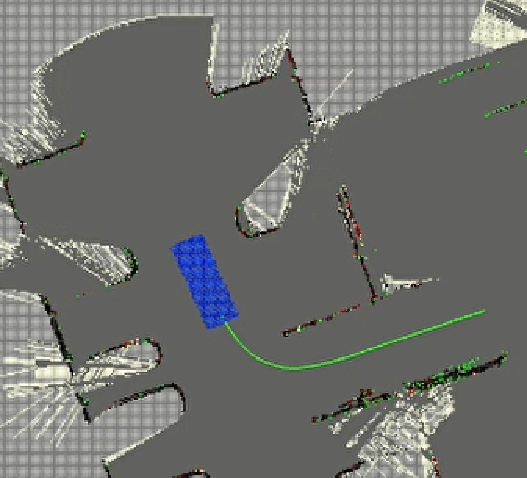
\includegraphics[width=0.7\textwidth]{pics/path.pdf}
	\caption{Visualisierung von Bewegungspfaden}
	\vspace{10in}
	\label{fig:path}
\end{figure}
Diese Funktion kann als Werkzeug verwendet werden, das w�hrend der tats�chlichen Pfadplanung aufgerufen wird.

\bibliographystyle{alphadin}
\bibliography{Literatur}
\setcounter{secnumdepth}{-1}
\section{Anhang}
\setcounter{secnumdepth}{3}
\renewcommand{\thefigure}{A\arabic{figure}}
\setcounter{figure}{0}
\subsection*{Abbildungen von Frequenz�berpr�fung}
\begin{figure}[htbp] 
	\centering
	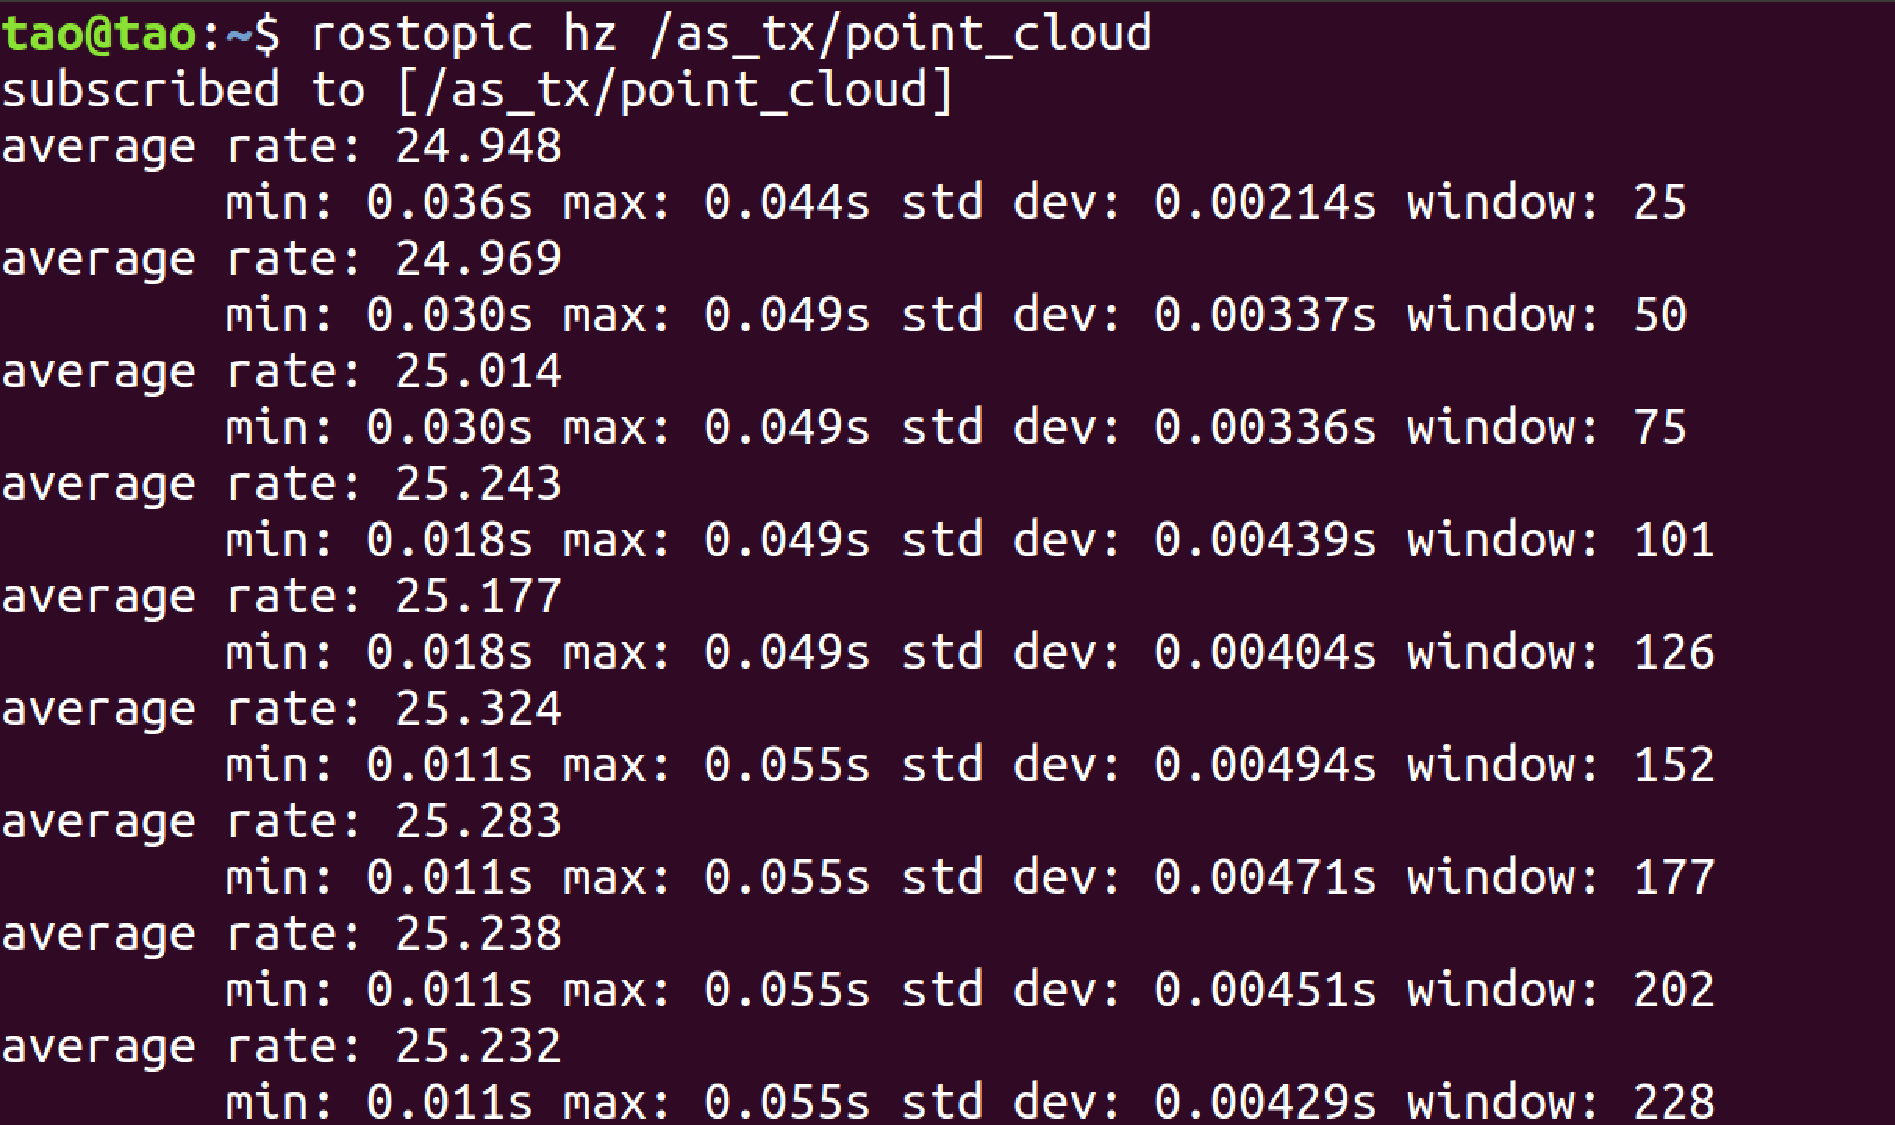
\includegraphics[width=0.8\textwidth]{pics/F_PCL.pdf}
	\caption{Frequenz von Information �ber Punktwolke}
	\label{fig:F_PCL}
\end{figure}
\begin{figure}[htbp] 
	\centering
	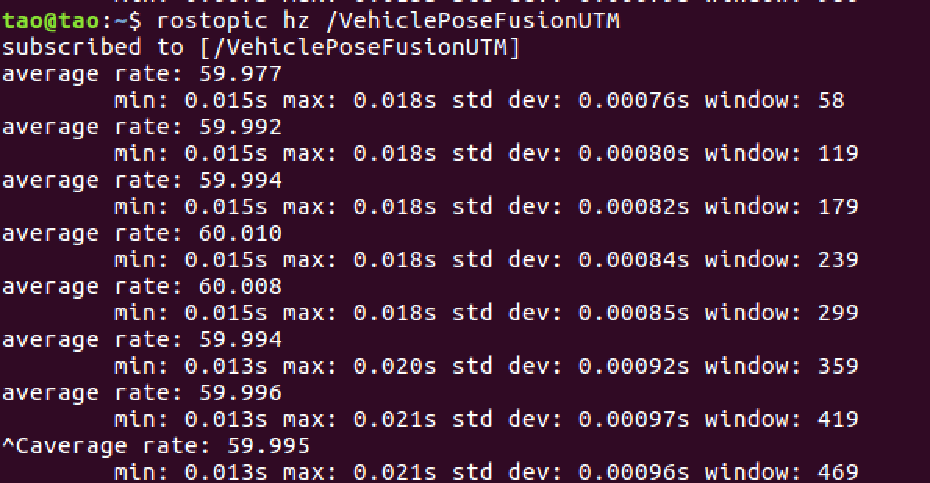
\includegraphics[width=0.8\textwidth]{pics/F_UTM.pdf}
	\caption{Frequenz von Information �ber UTM-Koordinaten}
	\label{fig:F_UTM}
\end{figure}
\begin{figure}[htbp] 
	\centering
	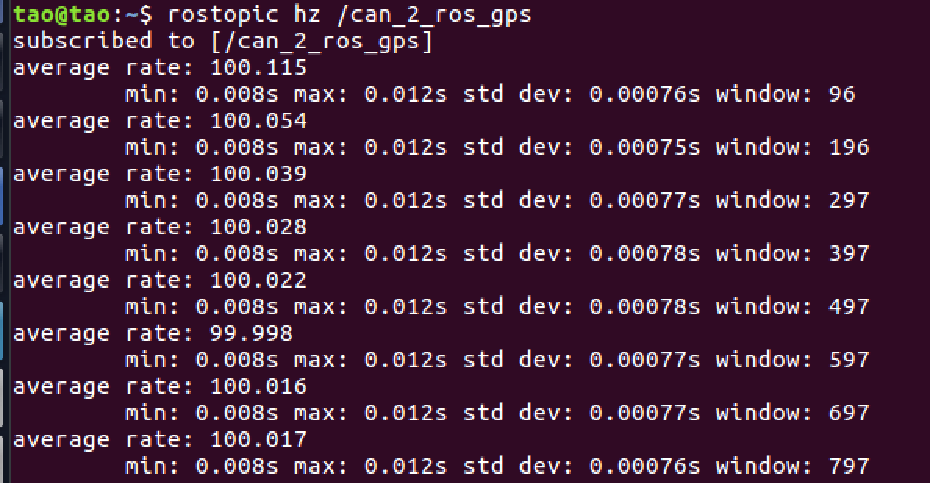
\includegraphics[width=0.9\textwidth]{pics/F_can_gsps.pdf}
	\caption{Frequenz von Information �ber Nickelwinkel}
	\label{fig:F_can_gsps}
\end{figure}
\begin{figure}[htbp] 
	\centering
	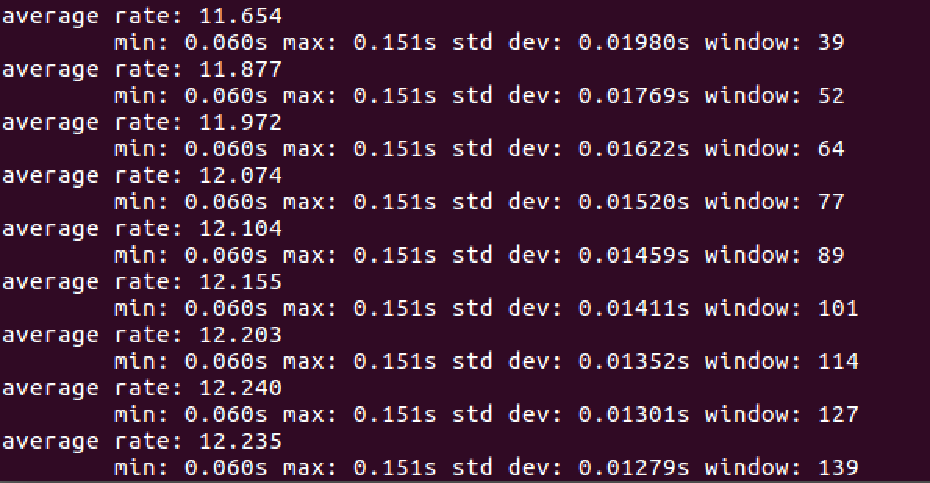
\includegraphics[width=0.9\textwidth]{pics/OUTPUT12Hz.pdf}
	\caption{Frequenz der Modellausgangsdaten}
	\label{fig:OUTPUT12Hz}
\end{figure} 

\end{document}
